
%% bare_jrnl_compsoc.tex
%% V1.4b
%% 2015/08/26
%% by Michael Shell
%% See:
%% http://www.michaelshell.org/
%% for current contact information.
%%
%% This is a skeleton file demonstrating the use of IEEEtran.cls
%% (requires IEEEtran.cls version 1.8b or later) with an IEEE
%% Computer Society journal paper.
%%
%% Support sites:
%% http://www.michaelshell.org/tex/ieeetran/
%% http://www.ctan.org/pkg/ieeetran
%% and
%% http://www.ieee.org/

%%*************************************************************************
%% Legal Notice:
%% This code is offered as-is without any warranty either expressed or
%% implied; without even the implied warranty of MERCHANTABILITY or
%% FITNESS FOR A PARTICULAR PURPOSE! 
%% User assumes all risk.
%% In no event shall the IEEE or any contributor to this code be liable for
%% any damages or losses, including, but not limited to, incidental,
%% consequential, or any other damages, resulting from the use or misuse
%% of any information contained here.
%%
%% All comments are the opinions of their respective authors and are not
%% necessarily endorsed by the IEEE.
%%
%% This work is distributed under the LaTeX Project Public License (LPPL)
%% ( http://www.latex-project.org/ ) version 1.3, and may be freely used,
%% distributed and modified. A copy of the LPPL, version 1.3, is included
%% in the base LaTeX documentation of all distributions of LaTeX released
%% 2003/12/01 or later.
%% Retain all contribution notices and credits.
%% ** Modified files should be clearly indicated as such, including  **
%% ** renaming them and changing author support contact information. **
%%*************************************************************************


% *** Authors should verify (and, if needed, correct) their LaTeX system  ***
% *** with the testflow diagnostic prior to trusting their LaTeX platform ***
% *** with production work. The IEEE's font choices and paper sizes can   ***
% *** trigger bugs that do not appear when using other class files.       ***                          ***
% The testflow support page is at:
% http://www.michaelshell.org/tex/testflow/


\documentclass[10pt,journal,compsoc]{IEEEtran}
%
% If IEEEtran.cls has not been installed into the LaTeX system files,
% manually specify the path to it like:
% \documentclass[10pt,journal,compsoc]{../sty/IEEEtran}
\usepackage{color}
\usepackage{epsfig,endnotes}
\usepackage{dblfloatfix}
\usepackage{float}
\usepackage{xspace}
\usepackage{url}
\usepackage{subfigure} 
\usepackage{epstopdf}
\usepackage{inlinenum}
\usepackage{amsmath}
\usepackage{array} 
\usepackage[export]{adjustbox}
\usepackage{multirow}
\usepackage{amssymb}
\setcounter{tocdepth}{3}
\usepackage{graphicx}

%\usepackage{breakurl} 
\usepackage[breaklinks]{hyperref}

\usepackage{url}
\urldef{\mailsa}\path|{alfred.hofmann, ursula.barth, ingrid.haas, frank.holzwarth,|
\urldef{\mailsb}\path|anna.kramer, leonie.kunz, christine.reiss, nicole.sator,|
\urldef{\mailsc}\path|erika.siebert-cole, peter.strasser, lncs}@springer.com|    
%\newcommand{\keywords}[1]{\par\addvspace\baselineskip\noindent\keywordname\enspace\ignorespaces#1}

\newcommand{\CiT}{\texttt{MoCRA}\xspace}
\newcommand{\figref}[1]{Figure~\ref{#1}}
\newcommand{\secref}[1]{Section~\ref{#1}}
\newcommand{\etal}{\mbox{\emph{et al.}}}
\newcommand{\jing}[1]{{\color{black}{#1}}}
\newcommand{\jingjuly}[1]{{\color{blue}{#1}}}
\newcommand{\jingap}[1]{{\color{black}{#1}}}
\newcommand{\jingnew}[1]{{\color{black}{#1}}}
\newcommand{\jingfeb}[1]{{\color{black}{#1}}}

\newcommand{\red}[1]{\color{}{#1}}




% Some very useful LaTeX packages include:
% (uncomment the ones you want to load)


% *** MISC UTILITY PACKAGES ***
%
%\usepackage{ifpdf}
% Heiko Oberdiek's ifpdf.sty is very useful if you need conditional
% compilation based on whether the output is pdf or dvi.
% usage:
% \ifpdf
%   % pdf code
% \else
%   % dvi code
% \fi
% The latest version of ifpdf.sty can be obtained from:
% http://www.ctan.org/pkg/ifpdf
% Also, note that IEEEtran.cls V1.7 and later provides a builtin
% \ifCLASSINFOpdf conditional that works the same way.
% When switching from latex to pdflatex and vice-versa, the compiler may
% have to be run twice to clear warning/error messages.






% *** CITATION PACKAGES ***
%
\ifCLASSOPTIONcompsoc
  % IEEE Computer Society needs nocompress option
  % requires cite.sty v4.0 or later (November 2003)
  \usepackage[nocompress]{cite}
\else
  % normal IEEE
  \usepackage{cite}
\fi
% cite.sty was written by Donald Arseneau
% V1.6 and later of IEEEtran pre-defines the format of the cite.sty package
% \cite{} output to follow that of the IEEE. Loading the cite package will
% result in citation numbers being automatically sorted and properly
% "compressed/ranged". e.g., [1], [9], [2], [7], [5], [6] without using
% cite.sty will become [1], [2], [5]--[7], [9] using cite.sty. cite.sty's
% \cite will automatically add leading space, if needed. Use cite.sty's
% noadjust option (cite.sty V3.8 and later) if you want to turn this off
% such as if a citation ever needs to be enclosed in parenthesis.
% cite.sty is already installed on most LaTeX systems. Be sure and use
% version 5.0 (2009-03-20) and later if using hyperref.sty.
% The latest version can be obtained at:
% http://www.ctan.org/pkg/cite
% The documentation is contained in the cite.sty file itself.
%
% Note that some packages require special options to format as the Computer
% Society requires. In particular, Computer Society  papers do not use
% compressed citation ranges as is done in typical IEEE papers
% (e.g., [1]-[4]). Instead, they list every citation separately in order
% (e.g., [1], [2], [3], [4]). To get the latter we need to load the cite
% package with the nocompress option which is supported by cite.sty v4.0
% and later. Note also the use of a CLASSOPTION conditional provided by
% IEEEtran.cls V1.7 and later.





% *** GRAPHICS RELATED PACKAGES ***
%
\ifCLASSINFOpdf
  % \usepackage[pdftex]{graphicx}
  % declare the path(s) where your graphic files are
  % \graphicspath{{../pdf/}{../jpeg/}}
  % and their extensions so you won't have to specify these with
  % every instance of \includegraphics
  % \DeclareGraphicsExtensions{.pdf,.jpeg,.png}
\else
  % or other class option (dvipsone, dvipdf, if not using dvips). graphicx
  % will default to the driver specified in the system graphics.cfg if no
  % driver is specified.
  % \usepackage[dvips]{graphicx}
  % declare the path(s) where your graphic files are
  % \graphicspath{{../eps/}}
  % and their extensions so you won't have to specify these with
  % every instance of \includegraphics
  % \DeclareGraphicsExtensions{.eps}
\fi
% graphicx was written by David Carlisle and Sebastian Rahtz. It is
% required if you want graphics, photos, etc. graphicx.sty is already
% installed on most LaTeX systems. The latest version and documentation
% can be obtained at: 
% http://www.ctan.org/pkg/graphicx
% Another good source of documentation is "Using Imported Graphics in
% LaTeX2e" by Keith Reckdahl which can be found at:
% http://www.ctan.org/pkg/epslatex
%
% latex, and pdflatex in dvi mode, support graphics in encapsulated
% postscript (.eps) format. pdflatex in pdf mode supports graphics
% in .pdf, .jpeg, .png and .mps (metapost) formats. Users should ensure
% that all non-photo figures use a vector format (.eps, .pdf, .mps) and
% not a bitmapped formats (.jpeg, .png). The IEEE frowns on bitmapped formats
% which can result in "jaggedy"/blurry rendering of lines and letters as
% well as large increases in file sizes.
%
% You can find documentation about the pdfTeX application at:
% http://www.tug.org/applications/pdftex






% *** MATH PACKAGES ***
%
%\usepackage{amsmath}
% A popular package from the American Mathematical Society that provides
% many useful and powerful commands for dealing with mathematics.
%
% Note that the amsmath package sets \interdisplaylinepenalty to 10000
% thus preventing page breaks from occurring within multiline equations. Use:
%\interdisplaylinepenalty=2500
% after loading amsmath to restore such page breaks as IEEEtran.cls normally
% does. amsmath.sty is already installed on most LaTeX systems. The latest
% version and documentation can be obtained at:
% http://www.ctan.org/pkg/amsmath





% *** SPECIALIZED LIST PACKAGES ***
%
%\usepackage{algorithmic}
% algorithmic.sty was written by Peter Williams and Rogerio Brito.
% This package provides an algorithmic environment fo describing algorithms.
% You can use the algorithmic environment in-text or within a figure
% environment to provide for a floating algorithm. Do NOT use the algorithm
% floating environment provided by algorithm.sty (by the same authors) or
% algorithm2e.sty (by Christophe Fiorio) as the IEEE does not use dedicated
% algorithm float types and packages that provide these will not provide
% correct IEEE style captions. The latest version and documentation of
% algorithmic.sty can be obtained at:
% http://www.ctan.org/pkg/algorithms
% Also of interest may be the (relatively newer and more customizable)
% algorithmicx.sty package by Szasz Janos:
% http://www.ctan.org/pkg/algorithmicx




% *** ALIGNMENT PACKAGES ***
%
%\usepackage{array}
% Frank Mittelbach's and David Carlisle's array.sty patches and improves
% the standard LaTeX2e array and tabular environments to provide better
% appearance and additional user controls. As the default LaTeX2e table
% generation code is lacking to the point of almost being broken with
% respect to the quality of the end results, all users are strongly
% advised to use an enhanced (at the very least that provided by array.sty)
% set of table tools. array.sty is already installed on most systems. The
% latest version and documentation can be obtained at:
% http://www.ctan.org/pkg/array


% IEEEtran contains the IEEEeqnarray family of commands that can be used to
% generate multiline equations as well as matrices, tables, etc., of high
% quality.




% *** SUBFIGURE PACKAGES ***
%\ifCLASSOPTIONcompsoc
%  \usepackage[caption=false,font=footnotesize,labelfont=sf,textfont=sf]{subfig}
%\else
%  \usepackage[caption=false,font=footnotesize]{subfig}
%\fi
% subfig.sty, written by Steven Douglas Cochran, is the modern replacement
% for subfigure.sty, the latter of which is no longer maintained and is
% incompatible with some LaTeX packages including fixltx2e. However,
% subfig.sty requires and automatically loads Axel Sommerfeldt's caption.sty
% which will override IEEEtran.cls' handling of captions and this will result
% in non-IEEE style figure/table captions. To prevent this problem, be sure
% and invoke subfig.sty's "caption=false" package option (available since
% subfig.sty version 1.3, 2005/06/28) as this is will preserve IEEEtran.cls
% handling of captions.
% Note that the Computer Society format requires a sans serif font rather
% than the serif font used in traditional IEEE formatting and thus the need
% to invoke different subfig.sty package options depending on whether
% compsoc mode has been enabled.
%
% The latest version and documentation of subfig.sty can be obtained at:
% http://www.ctan.org/pkg/subfig




% *** FLOAT PACKAGES ***
%
%\usepackage{fixltx2e}
% fixltx2e, the successor to the earlier fix2col.sty, was written by
% Frank Mittelbach and David Carlisle. This package corrects a few problems
% in the LaTeX2e kernel, the most notable of which is that in current
% LaTeX2e releases, the ordering of single and double column floats is not
% guaranteed to be preserved. Thus, an unpatched LaTeX2e can allow a
% single column figure to be placed prior to an earlier double column
% figure.
% Be aware that LaTeX2e kernels dated 2015 and later have fixltx2e.sty's
% corrections already built into the system in which case a warning will
% be issued if an attempt is made to load fixltx2e.sty as it is no longer
% needed.
% The latest version and documentation can be found at:
% http://www.ctan.org/pkg/fixltx2e


%\usepackage{stfloats}
% stfloats.sty was written by Sigitas Tolusis. This package gives LaTeX2e
% the ability to do double column floats at the bottom of the page as well
% as the top. (e.g., "\begin{figure*}[!b]" is not normally possible in
% LaTeX2e). It also provides a command:
%\fnbelowfloat
% to enable the placement of footnotes below bottom floats (the standard
% LaTeX2e kernel puts them above bottom floats). This is an invasive package
% which rewrites many portions of the LaTeX2e float routines. It may not work
% with other packages that modify the LaTeX2e float routines. The latest
% version and documentation can be obtained at:
% http://www.ctan.org/pkg/stfloats
% Do not use the stfloats baselinefloat ability as the IEEE does not allow
% \baselineskip to stretch. Authors submitting work to the IEEE should note
% that the IEEE rarely uses double column equations and that authors should try
% to avoid such use. Do not be tempted to use the cuted.sty or midfloat.sty
% packages (also by Sigitas Tolusis) as the IEEE does not format its papers in
% such ways.
% Do not attempt to use stfloats with fixltx2e as they are incompatible.
% Instead, use Morten Hogholm'a dblfloatfix which combines the features
% of both fixltx2e and stfloats:
%
% \usepackage{dblfloatfix}
% The latest version can be found at:
% http://www.ctan.org/pkg/dblfloatfix




%\ifCLASSOPTIONcaptionsoff
%  \usepackage[nomarkers]{endfloat}
% \let\MYoriglatexcaption\caption
% \renewcommand{\caption}[2][\relax]{\MYoriglatexcaption[#2]{#2}}
%\fi
% endfloat.sty was written by James Darrell McCauley, Jeff Goldberg and 
% Axel Sommerfeldt. This package may be useful when used in conjunction with 
% IEEEtran.cls'  captionsoff option. Some IEEE journals/societies require that
% submissions have lists of figures/tables at the end of the paper and that
% figures/tables without any captions are placed on a page by themselves at
% the end of the document. If needed, the draftcls IEEEtran class option or
% \CLASSINPUTbaselinestretch interface can be used to increase the line
% spacing as well. Be sure and use the nomarkers option of endfloat to
% prevent endfloat from "marking" where the figures would have been placed
% in the text. The two hack lines of code above are a slight modification of
% that suggested by in the endfloat docs (section 8.4.1) to ensure that
% the full captions always appear in the list of figures/tables - even if
% the user used the short optional argument of \caption[]{}.
% IEEE papers do not typically make use of \caption[]'s optional argument,
% so this should not be an issue. A similar trick can be used to disable
% captions of packages such as subfig.sty that lack options to turn off
% the subcaptions:
% For subfig.sty:
% \let\MYorigsubfloat\subfloat
% \renewcommand{\subfloat}[2][\relax]{\MYorigsubfloat[]{#2}}
% However, the above trick will not work if both optional arguments of
% the \subfloat command are used. Furthermore, there needs to be a
% description of each subfigure *somewhere* and endfloat does not add
% subfigure captions to its list of figures. Thus, the best approach is to
% avoid the use of subfigure captions (many IEEE journals avoid them anyway)
% and instead reference/explain all the subfigures within the main caption.
% The latest version of endfloat.sty and its documentation can obtained at:
% http://www.ctan.org/pkg/endfloat
%
% The IEEEtran \ifCLASSOPTIONcaptionsoff conditional can also be used
% later in the document, say, to conditionally put the References on a 
% page by themselves.




% *** PDF, URL AND HYPERLINK PACKAGES ***
%
%\usepackage{url}
% url.sty was written by Donald Arseneau. It provides better support for
% handling and breaking URLs. url.sty is already installed on most LaTeX
% systems. The latest version and documentation can be obtained at:
% http://www.ctan.org/pkg/url
% Basically, \url{my_url_here}.





% *** Do not adjust lengths that control margins, column widths, etc. ***
% *** Do not use packages that alter fonts (such as pslatex).         ***
% There should be no need to do such things with IEEEtran.cls V1.6 and later.
% (Unless specifically asked to do so by the journal or conference you plan
% to submit to, of course. )


% correct bad hyphenation here
\hyphenation{op-tical net-works semi-conduc-tor}


\begin{document}


%
% paper title
% Titles are generally capitalized except for words such as a, an, and, as,
% at, but, by, for, in, nor, of, on, or, the, to and up, which are usually
% not capitalized unless they are the first or last word of the title.
% Linebreaks \\ can be used within to get better formatting as desired.
% Do not put math or special symbols in the title.
\title{Challenge-Response Authentication using \\ \jing{ In-Air Handwriting Style Verification} }
%
%
% author names and IEEE memberships
% note positions of commas and nonbreaking spaces ( ~ ) LaTeX will not break
% a structure at a ~ so this keeps an author's name from being broken across
% two lines.
% use \thanks{} to gain access to the first footnote area
% a separate \thanks must be used for each paragraph as LaTeX2e's \thanks
% was not built to handle multiple paragraphs
%
%
%\IEEEcompsocitemizethanks is a special \thanks that produces the bulleted
% lists the Computer Society journals use for "first footnote" author
% affiliations. Use \IEEEcompsocthanksitem which works much like \item
% for each affiliation group. When not in compsoc mode,
% \IEEEcompsocitemizethanks becomes like \thanks and
% \IEEEcompsocthanksitem becomes a line break with idention. This
% facilitates dual compilation, although admittedly the differences in the
% desired content of \author between the different types of papers makes a
% one-size-fits-all approach a daunting prospect. For instance, compsoc 
% journal papers have the author affiliations above the "Manuscript
% received ..."  text while in non-compsoc journals this is reversed. Sigh.

\author{Jing Tian,
        Yu Cao,
        Wenyuan Xu,
        Song Wang% <-this % stops a space
\IEEEcompsocitemizethanks{\IEEEcompsocthanksitem Dept. of Computer Science and Engineering, University of South Carolina, Columbia, SC, 29208.\protect\\
% note need leading \protect in front of \\ to get a newline within \thanks as
% \\ is fragile and will error, could use \hfil\break instead.
E-mails: tian9@cec.sc.edu, cao@cec.sc.edu, wyxu@zju.edu.cn, songwang@cec.sc.edu }
%\IEEEcompsocthanksitem J. Doe and J. Doe are with Anonymous University.}% <-this % stops an unwanted space
\thanks{Manuscript received XXX XX, 2016; revised XXX XX, 2017.}}

% note the % following the last \IEEEmembership and also \thanks - 
% these prevent an unwanted space from occurring between the last author name
% and the end of the author line. i.e., if you had this:
% 
% \author{....lastname \thanks{...} \thanks{...} }
%                     ^------------^------------^----Do not want these spaces!
%
% a space would be appended to the last name and could cause every name on that
% line to be shifted left slightly. This is one of those "LaTeX things". For
% instance, "\textbf{A} \textbf{B}" will typeset as "A B" not "AB". To get
% "AB" then you have to do: "\textbf{A}\textbf{B}"
% \thanks is no different in this regard, so shield the last } of each \thanks
% that ends a line with a % and do not let a space in before the next \thanks.
% Spaces after \IEEEmembership other than the last one are OK (and needed) as
% you are supposed to have spaces between the names. For what it is worth,
% this is a minor point as most people would not even notice if the said evil
% space somehow managed to creep in.



% The paper headers
\markboth{IEEE Transactions on Dependable and Secure Computing,~Vol.~XXX, No.~XXX, XXXXX~2017}%
{Shell \MakeLowercase{\textit{et al.}}: Bare Demo of IEEEtran.cls for Computer Society Journals}
% The only time the second header will appear is for the odd numbered pages
% after the title page when using the twoside option.
% 
% *** Note that you probably will NOT want to include the author's ***
% *** name in the headers of peer review papers.                   ***
% You can use \ifCLASSOPTIONpeerreview for conditional compilation here if
% you desire.



% The publisher's ID mark at the bottom of the page is less important with
% Computer Society journal papers as those publications place the marks
% outside of the main text columns and, therefore, unlike regular IEEE
% journals, the available text space is not reduced by their presence.
% If you want to put a publisher's ID mark on the page you can do it like
% this:
%\IEEEpubid{0000--0000/00\$00.00~\copyright~2015 IEEE}
% or like this to get the Computer Society new two part style.
%\IEEEpubid{\makebox[\columnwidth]{\hfill 0000--0000/00/\$00.00~\copyright~2015 IEEE}%
%\hspace{\columnsep}\makebox[\columnwidth]{Published by the IEEE Computer Society\hfill}}
% Remember, if you use this you must call \IEEEpubidadjcol in the second
% column for its text to clear the IEEEpubid mark (Computer Society jorunal
% papers don't need this extra clearance.)



% use for special paper notices
%\IEEEspecialpapernotice{(Invited Paper)}



% for Computer Society papers, we must declare the abstract and index terms
% PRIOR to the title within the \IEEEtitleabstractindextext IEEEtran
% command as these need to go into the title area created by \maketitle.
% As a general rule, do not put math, special symbols or citations
% in the abstract or keywords.
\IEEEtitleabstractindextext{%
\begin{abstract}
Challenge-response (CR) is an effective way to authenticate users even if the communication channel is insecure. Tradition- ally, CR authentication relies on one-way hashes and shared secrets to verify the identities of users. Such a method cannot cope with an insider attack, where a user can obtained the secret \jingap{(i.e., the response)} from a legitimate user. To cope with it, we design a biome- tric-based CR authentication scheme (hereafter \CiT), which is derived from the motions as a user operates emerging depth-sensor- based input devices, such as a Leap Motion controller. We envision that to authenticate a user, \CiT randomly chooses a string (e.g., a few words), and the user has to write the string in the air. Using Leap Motion, \CiT captures the user's writing movements and then extracts his / her handwriting style. After verifying that what the user writes matches what is asked for, \CiT leverages a Support Vec- tor Machine (SVM) with co-occurrence matrices to model the handwriting styles and can reliably authenticate users, even if what they write is completely different every time. Evaluated on data from 24 subjects over 7 months, \CiT managed to verify a user with an average of $1.18\%$ (Equal Error Rate) EER and to reject \jingap{impostors}  with $2.45\%$ EER.
\end{abstract}

% Note that keywords are not normally used for peerreview papers.
\begin{IEEEkeywords}
%TODO
Authentication, challenge-response, identification, biometrics, SVM, handwriting style.
\end{IEEEkeywords}
}


% make the title area
\maketitle


% To allow for easy dual compilation without having to reenter the
% abstract/keywords data, the \IEEEtitleabstractindextext text will
% not be used in maketitle, but will appear (i.e., to be "transported")
% here as \IEEEdisplaynontitleabstractindextext when the compsoc 
% or transmag modes are not selected <OR> if conference mode is selected 
% - because all conference papers position the abstract like regular
% papers do.

%\IEEEdisplaynontitleabstractindextext

% \IEEEdisplaynontitleabstractindextext has no effect when using
% compsoc or transmag under a non-conference mode.



% For peer review papers, you can put extra information on the cover
% page as needed:
% \ifCLASSOPTIONpeerreview
% \begin{center} \bfseries EDICS Category: 3-BBND \end{center}
% \fi
%
% For peerreview papers, this IEEEtran command inserts a page break and
% creates the second title. It will be ignored for other modes.
\IEEEpeerreviewmaketitle

%\begin{abstract}
%70-150words
Challenge-response (CR) is an effective way to authenticate users even if the communication channel is insecure. Traditionally, CR authentication relies on one-way hashes and shared secrets to verify the identities of users. Such a method cannot cope with an insider attack, where a user obtained the secret from a legitimate user. To cope with it, we design a biometric-based CR authentication scheme (hereafter \CiT), which is derived from the motions as a user operates emerging depth-sensor-based input devices, such as a Leap Motion controller. We envision that to authenticate a user, \CiT randomly chooses a string (e.g., a few words), and the user has to write the string in the air. Utilizing Leap Motion, \CiT captures the user's writing movements and then extracts his handwriting style. After verifying that what the user writes matches what is asked for, \CiT leverages a Support Vector Machine (SVM) with co-occurrence matrices to model the handwriting styles and can correctly authenticate users, even if what they write is completely different every time. Evaluated on data from 24 subjects over 7 months, \CiT managed to verify a user with an average of $1.18\%$ (Equal Error Rate) EER and to reject imposers  with $2.26\%$ EER.



%\keywords{Authentication, challenge-response, biometrics, SVM, handwriting style, leap motion}

\end{abstract}
\IEEEraisesectionheading{\section{Introduction}\label{sec:introduction}}
\label{sec:intro}


%1. What is challenge response authentication, how does it work? What’s the typical flow?
%2 What are the advantages of challenge response authentication compared with other authentication scheme?
%3. What does the traditional challenge response authentication missing?  For instance, if I got my friend’s exxon mobile easy pay, I can get gasoline with his card.  This cannot prevent insider attacks. 

%For instance, only those guards who have passed background check can be authorized to walk throughout the building. Verifying their identities is important.  Therefore, we introduce a biometric-based challenge response scheme.  We don’t use fingerprint because of the privacy concern…….

%4. Why we use motion?  Because depth sensors becomes pervasive, and it is a behavor based biometrics
%5. Why it’s challenging, because we have to ask users to write different content yet still authenticate it correctly. 
%6. What’s our basic idea? model the writing style instead of what he/she writes…..


User authentication is one of the most important yet challenging tasks in computer security~\cite{Uell:CCS13,Monrose:CCS99,Zheng:CCS11,Ahmed:TPDS07,Ari:CCS13}. The difficulty stems from the insecure communication, where eavesdropping, man-in-the-middle attacks, and replay attacks are all made possible. Challenge-response (CR) authentication can effectively cope with these attacks: typically, during a CR authentication, one party (e.g., a server) sends a random challenge. To be authenticated, the other party (e.g., a user) has to send back a valid response, which is usually the hash of the challenge and the secret shared by the two parties beforehand. Because the challenge is randomly selected and it is difficult to extract the password from the response,  CR authentication is considered secure over insecure communication channels.  However, such a challenge response method authenticates is based on \textit{what you know} instead of \textit{who you are}. Anyone knowing the shared secret can pass the authentication. Such authentication cannot prevent insider attacks, which are serious threats to systems with strict security requirements. For instance, enterprise or government may only allow the security guards who have passed extensive background checks to patrol their buildings. Letting their friends or colleagues without background checks substitute them is not allowed and can lead to an insider attack. To address it, we study biometric-based challenge-response schemes to authenticate based on \textit{who you are}. \jing{Compared with authentication using biometrics, adding the procedure of challenge-response will introduce an extra amount of time to verify the response. Nevertheless, we believe the challenge-response procedure can reduce the possibility of replay attacks.}


\begin{figure}[t]
\vspace{-5mm}
\centering
{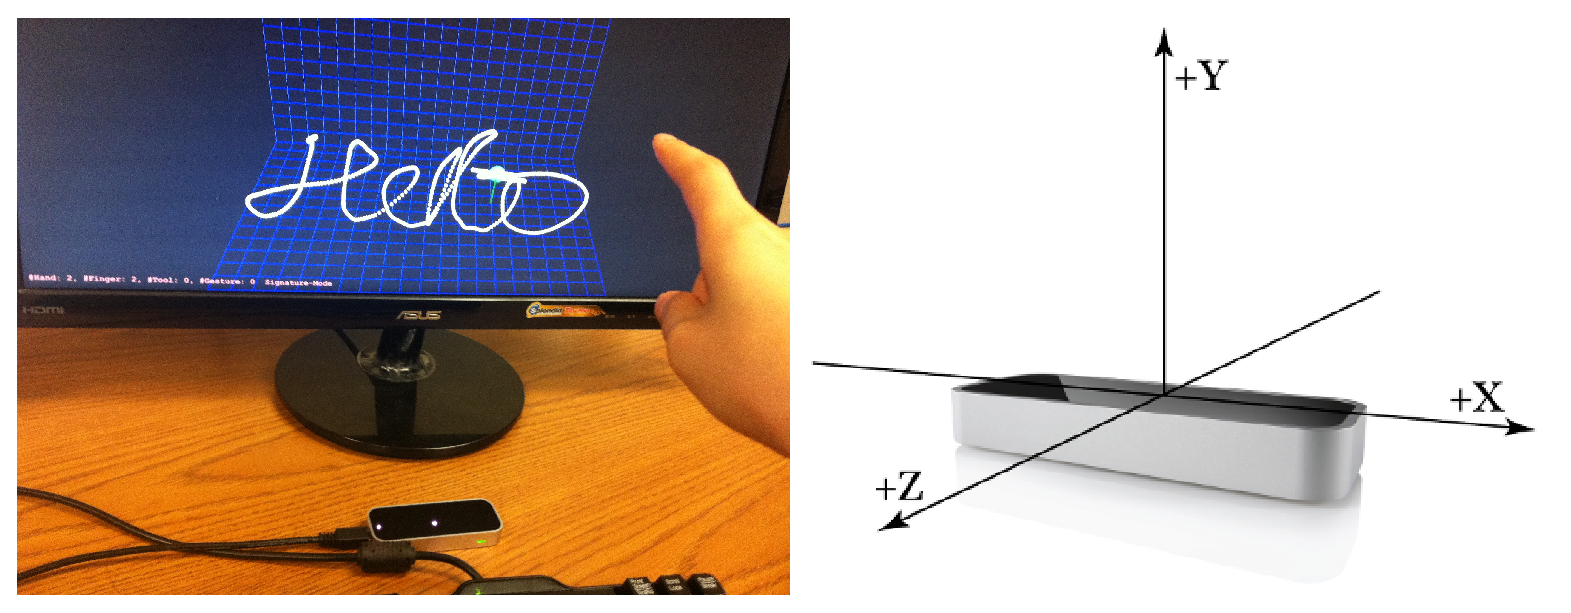
\includegraphics[width=.9\columnwidth]{./Graphic/SystemFlow/leap_motion_system.eps}} %LP.pdf
\caption{{An illustration of using a Leap Motion controller to acquire a user's handwriting in the 3D space for content independent CR authentication.}\vspace{-5mm}}\label{fig:leap}
\end{figure}





Both physical and behavioral biometrics can be used to identify who you are. Considering that physical biometrics are not privacy-friendly and are limited in numbers, we focus on designing a behavioral-biometric-based CR authentication system.
%\jing{We envision to design a motion-based authentication system with the following features. First, it works in a contactless manner, which has the benefit to elliminate hygiene concerns and is resilient to smudge attacks~\cite{Aviv:woot10}, i.e., finger smudges (due to oily residues) on a touch screen can reveal passwords. Second, it can be used as a complementary method when traditional biometrics-based authentication is inapplicable. For instance, fingerprints are inapplicable in several scenarios, e.g., fingerprints are unsuitable to users with dirty, greasy, or worn-out fingerprints due to their professions (e.g., miners). Third, it should be applicable to the public scenarios and thus should be resistant to shoulder surfing (i.e., observing) attacks, and acoustic environmental noises. } 
\jing{
We propose to use in-air handwriting style as a new biometrics for authentication. We use a depth motion sensor, Leap Motion controller~\cite{LeapOnline1} to record in-air fingertip writings as shown in Figure~\ref{fig:leap}. \jingap{Handwriting samples}, in the form of scanned images or recorded by tablet, have been used as signature verification or writer identification for authorization or forensics purpose~\cite{Schomaker:2008}. Compared to writings on tablet, the in-air writings introduce a larger amount of variability which we believe contain a richer set of biometric yet introduce extra intra-variance for multiple trial of writings from the same writer, and thus impose challenges for authentication. 

Despite of the challenge, we choose in-air handwriting because it has the following advantages. First, it does not require physical contact to any device. Thus, it elliminates hygiene concerns and is resilient to smudge attacks~\cite{Aviv:woot10}, i.e., finger smudges (due to oily residues) on a touch screen can reveal passwords.  Second, handwriting style is essentially a behavioral biometrics and thus has limited privacy issue. Third, given the rich combination of letters and numbers, the continuously written words are challenging to be synthesized because we believe that imitating arbitrary handwritings in the three dimensional (3D)-space is ambitious, making it resistant to shoulder surfing.}  Last but not least, it can be used as a complementary method when traditional biometrics-based authentication is inapplicable. For instance, fingerprints are inapplicable in several scenarios, e.g., fingerprints are unsuitable to users with dirty, greasy, or worn-out fingerprints due to their professions (e.g., miners). 


We call the proposed behavioral-biometric-based CR authentication system as \CiT. Specifically, we use data extracted from finger movements when a user writes in the air.
The \CiT system works as follows. To authenticate a user, \CiT randomly prompts a string (e.g., a few words) on the screen as a challenge, and the user has to write the string in the air as a response. Then the system performs two steps. First, determine whether the content of the handwriting is the same as the challenge. Second, verify if the handwriting is created by the user. Since  handwriting recognition can utilize existing technology~\cite{Tappert1990} and recent study shows that Leap Motion has the potential for handwriting recognition application~\cite{Vikram_handwritingleap, ICDAR15:OnlineHandwriting}, this paper focuses on the second step --- user verification based on the in-air handwriting. 


\begin{figure}[!t]
\centering
\begin{tabular}{cccccc}
\hline 
\vspace{2mm}
User-1
&
{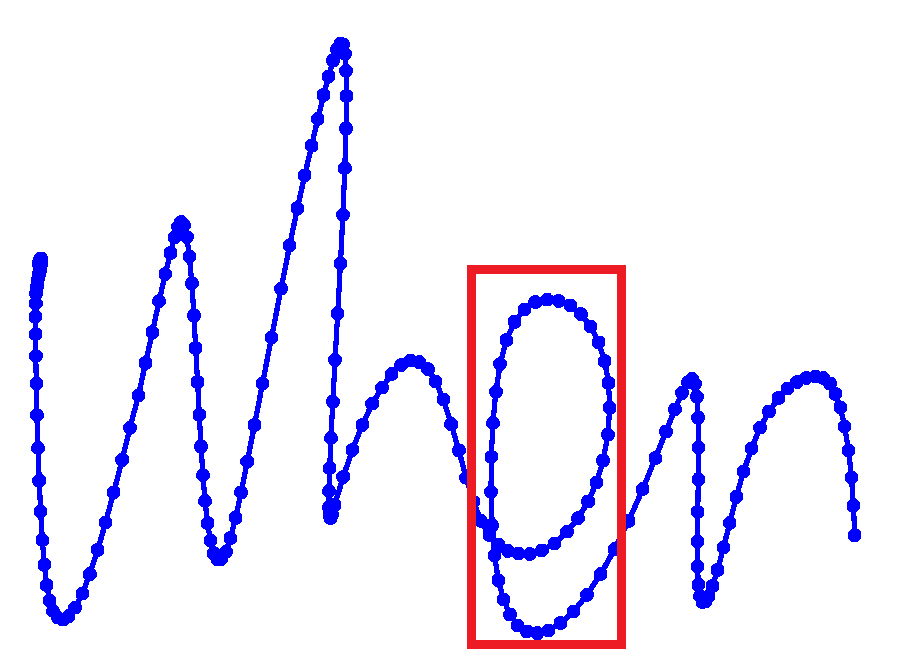
\includegraphics[width=0.09\columnwidth]{./Graphic/words_jing/1001_pdfCopy.eps}}
%&
%{
\includegraphics[width=0.09\columnwidth]{./Graphic/words_jing/1002_pdf.eps}}
& 
{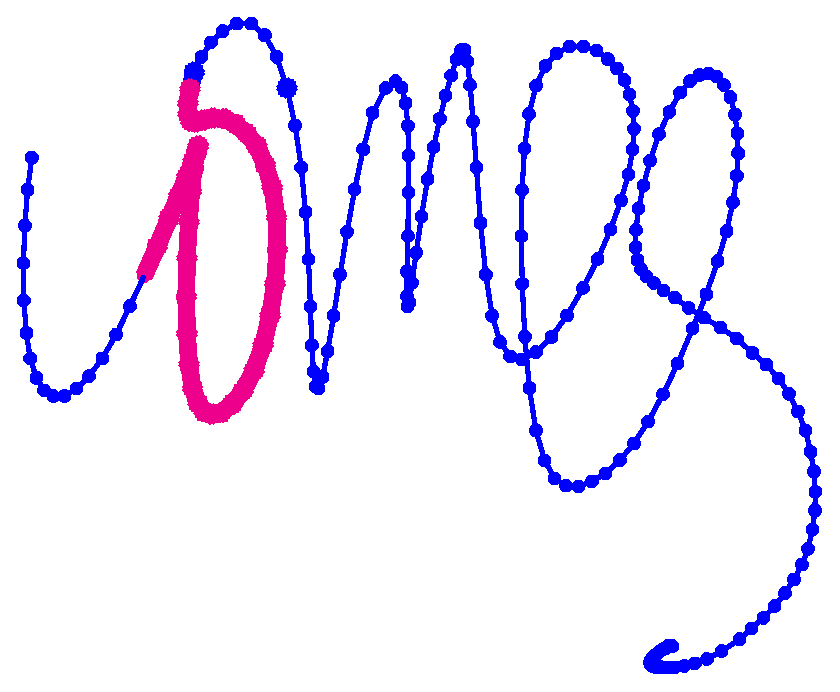
\includegraphics[width=0.09\columnwidth]{./Graphic/words_jing/1003_pdfCopy.eps}}
%& 
%{
\includegraphics[width=0.09\columnwidth]{./Graphic/words_jing/1004_pdfCopy.eps}}
%& 
%{
\includegraphics[width=0.19\columnwidth]{./Graphic/words_jing/1005_pdf.eps}}
%& 
%{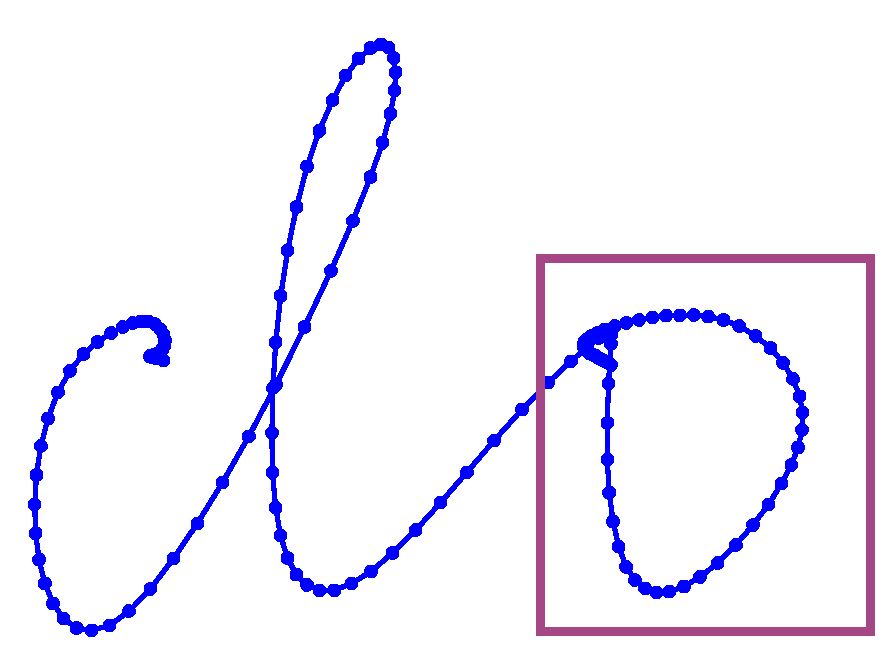
\includegraphics[width=0.09\columnwidth]{./Graphic/words_jing/1007_pdfCopy.eps}}
& 
{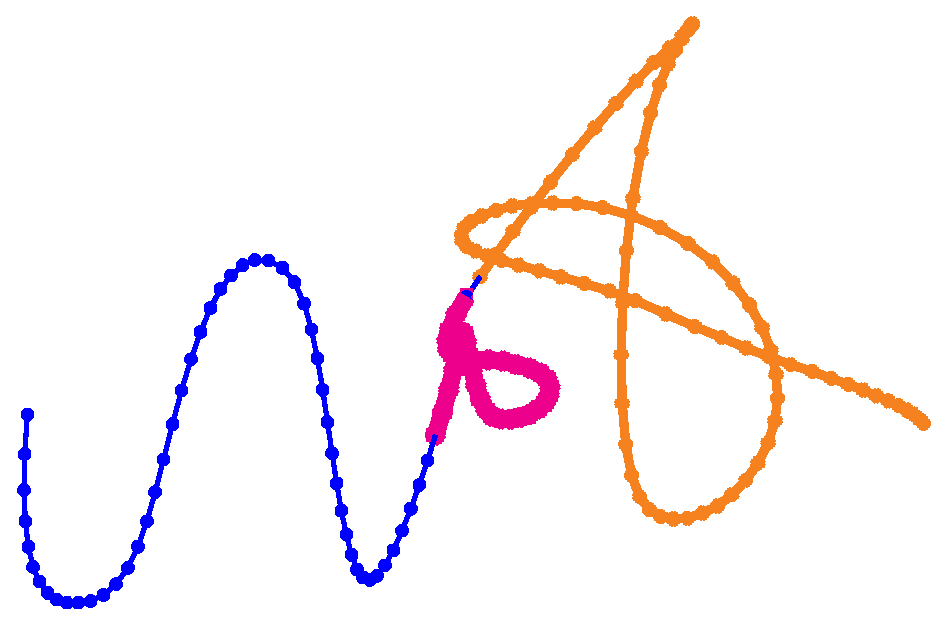
\includegraphics[width=0.09\columnwidth]{./Graphic/words_jing/1008_pdfCopy.eps}}
& 
{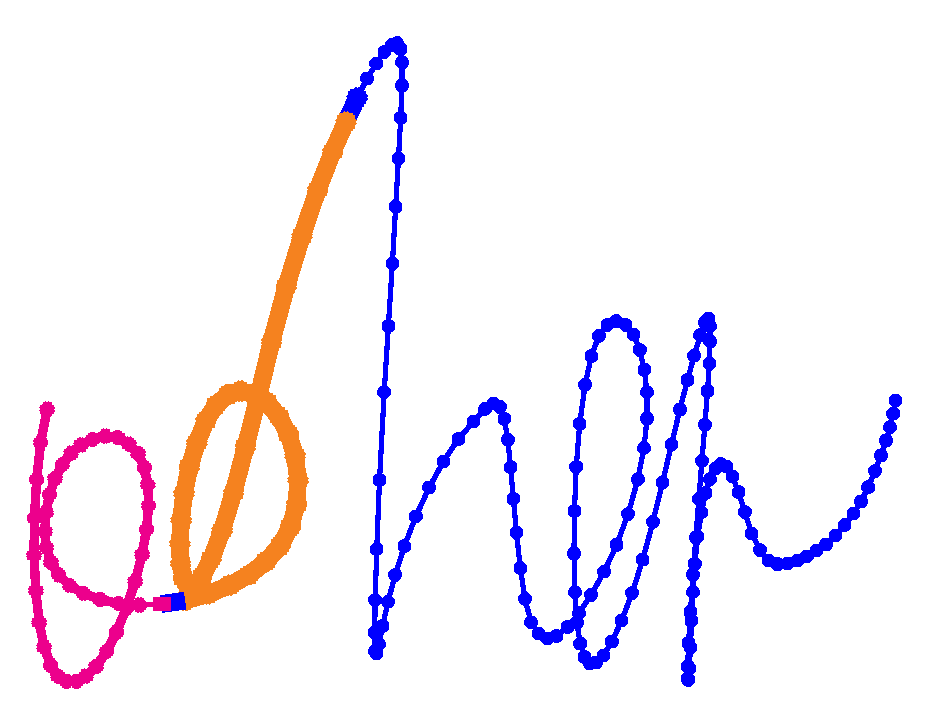
\includegraphics[width=0.09\columnwidth]{./Graphic/words_jing/1011_pdfCopy.eps}}
& 
{
\includegraphics[width=0.09\columnwidth]{./Graphic/words_jing/1014_pdfCopy.eps}}
\\ 

 & \texttt{when} %& \texttt{it} 
 & \texttt{comes} & \texttt{out}  & \texttt{other} & \texttt{but} \\ 
\hline 
%\vspace{3mm}
User-2
& 
{
\includegraphics[width=0.09\columnwidth]{./Graphic/words_meng/10023_pdf.eps}}
%&
%{
\includegraphics[width=0.09\columnwidth]{./Graphic/words_meng/10026_pdf.eps}}
& 
{
\includegraphics[width=0.09\columnwidth]{./Graphic/words_meng/10030_pdf.eps}}
%& 
%{
\includegraphics[width=0.09\columnwidth]{./Graphic/words_meng/20003_pdf.eps}}
%& 
%{
\includegraphics[width=0.09\columnwidth]{./Graphic/words_meng/20014_pdf.eps}}
%& 
%{
\includegraphics[width=0.09\columnwidth]{./Graphic/words_meng/20018_pdf.eps}}
& 
{
\includegraphics[width=0.09\columnwidth]{./Graphic/words_meng/20019_pdf.eps}}
& 
{
\includegraphics[width=0.09\columnwidth]{./Graphic/words_meng/20028_pdf.eps}}
& 
{
\includegraphics[width=0.09\columnwidth]{./Graphic/words_meng/20033_pdf.eps}}
\\ 
 & \texttt{as} %& \texttt{or} 
 & \texttt{with} & \texttt{makes}  & \texttt{some} & \texttt{even} \\ 
\hline
User-3
& 
{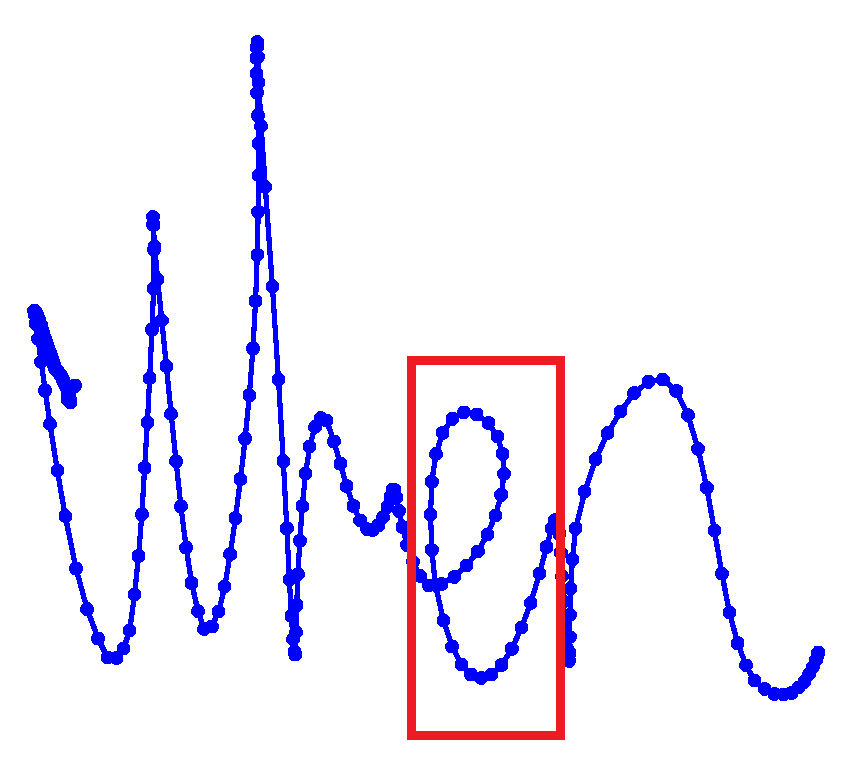
\includegraphics[width=0.09\columnwidth]{./Graphic/words_cao/10001_pdfCopy.eps}}
%&
%{
\includegraphics[width=0.09\columnwidth]{./Graphic/words_cao/10002_pdf.eps}}
& 
{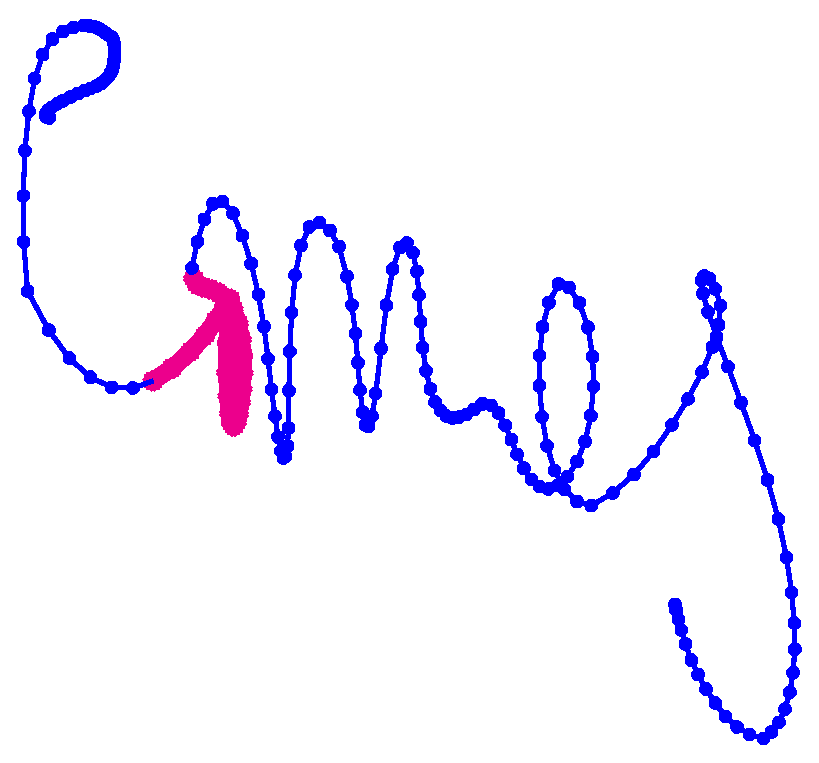
\includegraphics[width=0.09\columnwidth]{./Graphic/words_cao/10003_pdfCopy.eps}}
%& 
%{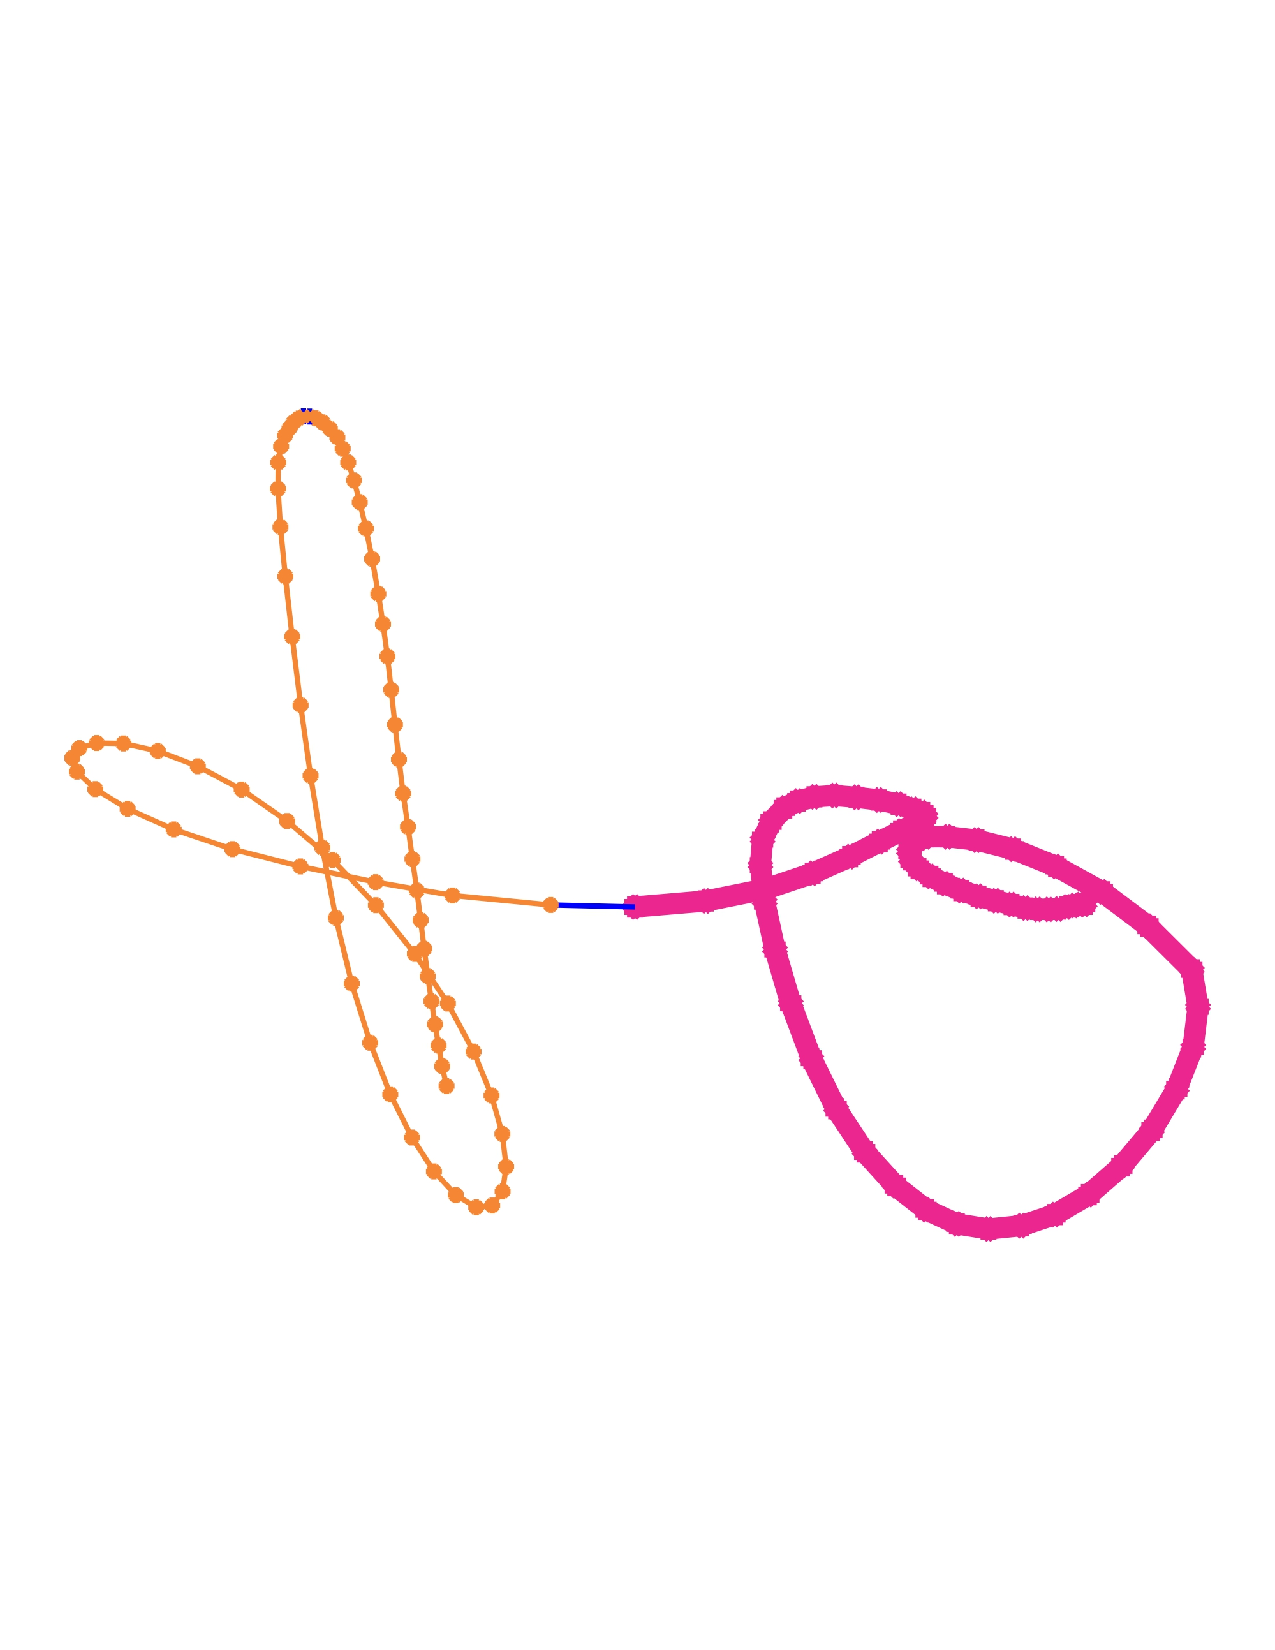
\includegraphics[width=0.09\columnwidth]{./Graphic/words_cao/10004_pdfCopy.pdf}}
%& 
%{
\includegraphics[width=0.09\columnwidth]{./Graphic/words_cao/10005_pdf.eps}}
%& 
%{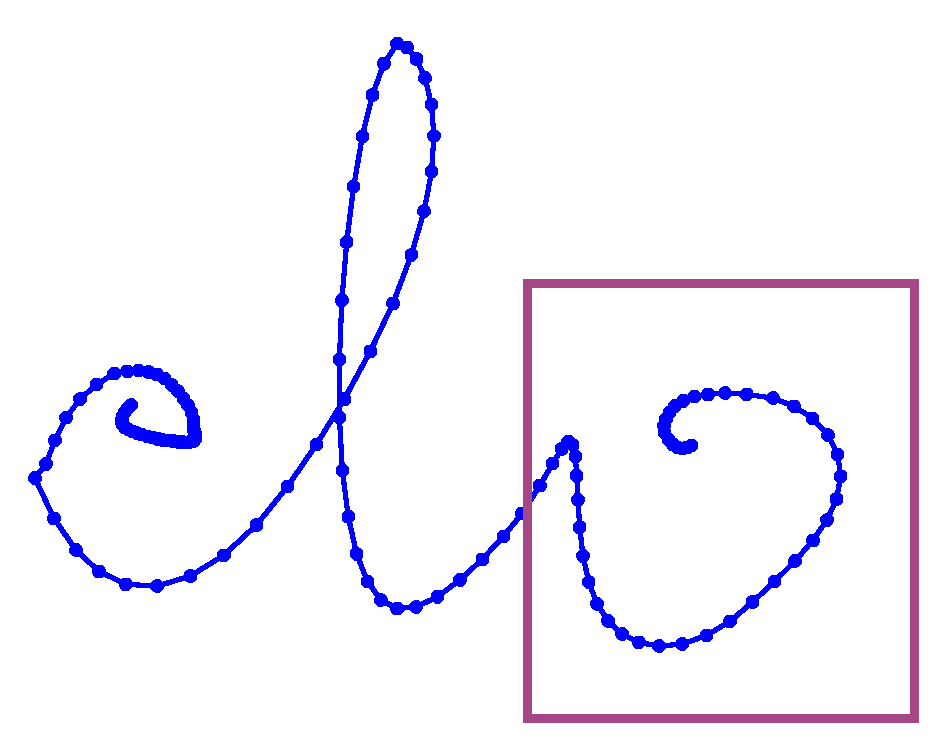
\includegraphics[width=0.09\columnwidth]{./Graphic/words_cao/10007_pdfCopy.eps}}
& 
{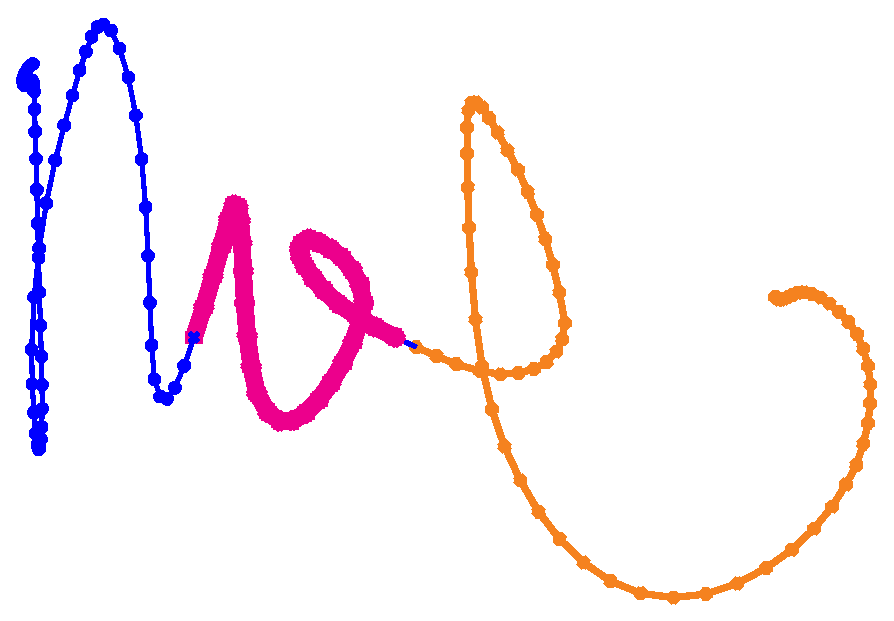
\includegraphics[width=0.09\columnwidth]{./Graphic/words_cao/10008_pdfCopy.eps}}
& 
{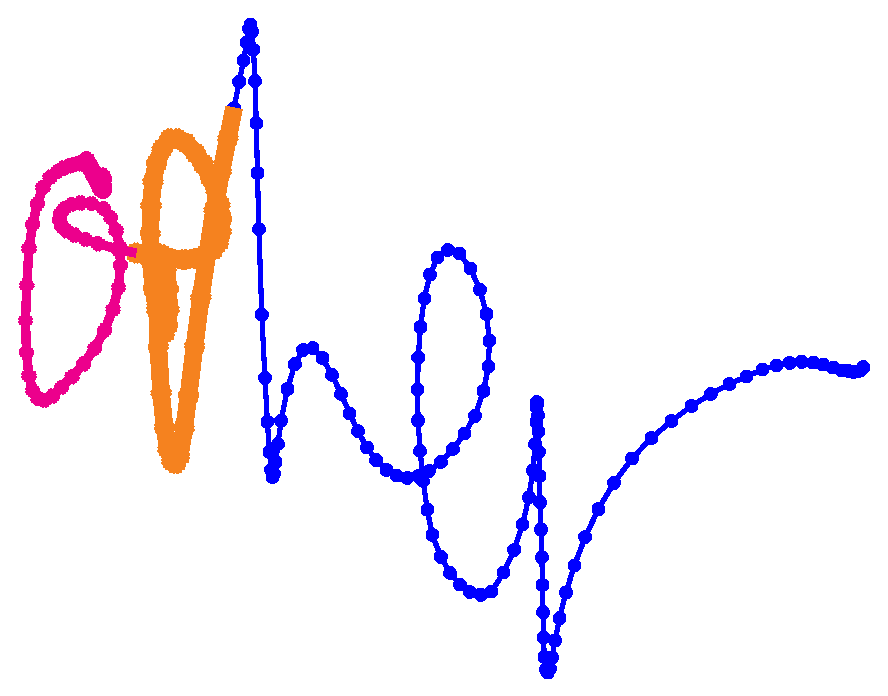
\includegraphics[width=0.09\columnwidth]{./Graphic/words_cao/10011_pdfCopy.eps}}
& 
{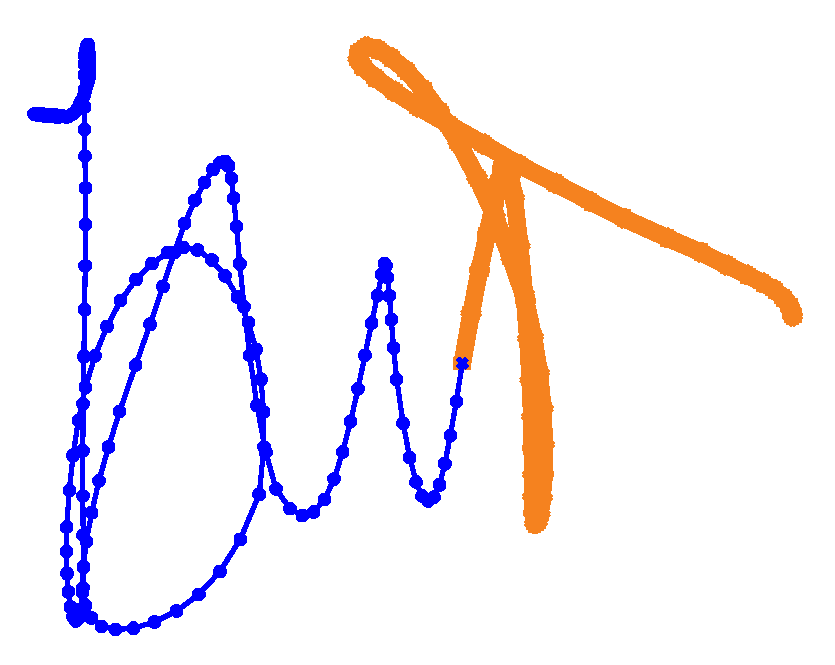
\includegraphics[width=0.09\columnwidth]{./Graphic/words_cao/10014_pdfCopy.eps}} 
\\ 
 & \texttt{when} %& \texttt{it} 
 & \texttt{comes} & \texttt{out}  & \texttt{other} & \texttt{but} \\ 
\hline
\end{tabular}
%\vspace{3mm}
\caption{\jing{Examples of processed trajectories written by two users. 
Despite that some handwritten words from User-1 and User-3 appear to be similar (e.g., \texttt{but}) yet some letters written by the same user may differ (e.g., the highlighted letters `o' and `t'), our authentication system can reliably distinguish them regardless of what they wrote. This is because \CiT is independent of text contents since it utilizes features derived at the scale of a stroke segment, e.g., \jingjuly{a short length of handwritten trajectory}.  
}\vspace{-3mm}}\label{fig:dataWords3user}

\end{figure}


%To track the motion of human fingers, we utilize depth sensors, because they are capable of capturing 3D human motion in a \textit{touch free} manner, just like how a camera captures pictures. Unlike behavior biometrics that rely on \textit{contact-based} input devices, such as touch screens~\cite{Kubota:ISPACS06,Liu:2009MobiHCI}, mouse movements~\cite{Zheng:CCS11,Ahmed:TPDS07}, keystroke dynamics~\cite{Monrose:CCS99,Revett:springerlink:10},  depth sensors eliminate hygiene concerns and smudge attacks~\cite{Aviv:woot10}.  Without loss of generality, we focus on utilizing a promising depth sensor --- a Leap Motion controller (in short, Leap Motion), which is designed to let users interact with a computer by waving their hands and fingers~\cite{LeapOnline1}, as shown in Figure~\ref{fig:leap}. Leap Motion captures the 3D motion of fingers at a relatively high precision 
%and tracks the finger length as well as width. This allows capturing behavior biometrics at a higher degree of freedom (i.e., entropy) than the traditional handwriting captured on flat surfaces (e.g., paper). 





%i.e., finger smudges (due to oily residues) on a touch screen can reveal passwords. In addition, unlike fingerprints, which are unsuitable to users with dirty, greasy, or worn-out fingerprints due to their professions (e.g., miners).


  

%Most of such biometrics is embedded in the usage pattern of various touch-based input devices, such as finger gestures when operating touch screens~\cite{Kubota:ISPACS06,Liu:2009MobiHCI}, mouse movements~\cite{Zheng:CCS11,Ahmed:TPDS07}, keystroke dynamics~\cite{Monrose:CCS99,Revett:springerlink:10}, etc. However, the recent advances in depth sensors has remarkably changed and will continue to alter the landscape of human-computer interaction. The trend urges us to explore new authentication schemes utilizing biometrics that is naturally built in the usage of the emerging depth sensors.

%, new input technologies, we explore new biometrics that can satisfy the re-authentication requirements that traditional text password and token-based authentication cannot offer.

%The emerge of low-cost depth sensors has remarkably changed and will continue to change the landscape of human-computer interaction, which was dominated by contact-based input devices, i.e., keyboards, mics, or touch screens. 
%Unlike contact-based input devices (i.e., touch screens~\cite{Kubota:ISPACS06,Liu:2009MobiHCI}, mouse movements~\cite{Zheng:CCS11,Ahmed:TPDS07}, keystroke dynamics~\cite{Monrose:CCS99,Revett:springerlink:10}), depth sensors are capable of capturing 3D human motion in a touch free manner, just like how a camera captures pictures. We have already witness how Microsoft Kinect~\cite{Kinect} and Leap Motion controller~\cite{LeapOnlineOverview} opened a new page for gaming and new apps. Looking forward, given that depth sensors enable a far less constrained input modalities than prior devices, they will become a non-dispensable part of future devices: Intel has announced to integrate RealSense 3D Cameras into mainstream computing devices~\cite{Intel}; Google has its plan of adding depth sensors into smartphones~\cite{Google}. In summary, the future human-computer interfaces are likely to be based on human motion, which simultaneously provides an opportunity for novel authentication schemes. 



%We design a new CS authentication scheme that is called \CiT, and the basic idea is to extract biometrics (also called \CiT) from finger movements when the user is writing in the air. When authenticate a user, the system randomly prompt a string on the screen as a challenge, and later the user write the string in the air as a response. The system authentication after receiving the response has two steps. First, recognize the handwriting to check if the content is the same as the challenge. Second, verify if the handwriting style is from a given user or from a given group of users. The handwriting recognition has been done by Tappert etc~\cite{Tappert1990}, thus our research focuses on the second part.



%To track the motion of human fingers as he/she writes in the air, without loss of generality, we focus on utilizing an emerging popular input device --- a Leap Motion controller (in short, Leap Motion), which is designed to let users interact with a computer by waving their hands and fingers~\cite{LeapOnline1}, as shown in Figure~\ref{fig:leap}.  


%Using depth sensors is advantageous: First, it captures the 3D motion of fingers %at a relatively high precision 
%and tracks the finger length as well as width. This allows capturing behavior biometrics at a higher degree of freedom (i.e., entropy) than the traditional handwriting captured on flat surfaces (e.g, paper). Second, operating in a contactless manner, it eliminates hygiene concerns and smudge attacks~\cite{Aviv:woot10}, i.e., finger smudges (due to oily residues) on a touch screen can reveal passwords. 
%Third, it is complementary to many traditional biometrics. For instance,   fingerprints have limitation and are inapplicable in several scenarios, e.g., fingerprints are unsuitable to users with dirty, greasy, or worn-out fingerprints due to their professions (e.g., miners).
%Forth, given the rich combination of letters and numbers, the continuously-written words are challenging to synthesize because imitating arbitrary handwriting in the 3 dimensional (3D)-space is ambitious. Thus, it is likely to be resistant to shoulder surfing. 
%Finally, writing words in the air might not be a completely natural way for entering information yet, but we optimistically predict that  users might adapt to it over time, similar to how users became familiar with keyboards. 




%We envision that \CiT can be used to authenticate users in a scenario insider attacker should be avoided. After initial user authentication, a user will receive a random string from the computer and interact with computers by writing towards a leap motion.
%%, since writing math symbols or formulas is preferable over typing. 
%Throughout the session, \CiT can harvest behavioral biometrics that is embedded in writing regardless of the writing content, so that it can verify users 
%% (i.e., identify a legitimate user out of a set of known candidates) 
%and raise an alarm when an alien is detected (i.e., an attacker tries to impersonate known candidates). 

%, who may share or have their individual motion depth sensors, enter comments by     some users may share the same input devices and enter comments by writing instead of typing, since writing math symbols or formulas is preferable over typing. In this case, it is promising to correctly exclude all aliens and identify each user regardless of what he/she writes, and inform the remote parties in real time. In summary, the goal is to perform re-authentication and have a high rejection rate for aliens and a high identification accuracy to determine user identity.% with a short delay.  



\CiT has to be \textit{content-independent} for CR authentication, because the CR authentication can require a user to write any content including letters, digits, and special symbols.
We design the second step of \CiT to rely on the handwriting style, i.e., authenticating based on `how you write' instead of `what you write'.   Building such an authentication system is challenging. First, extracting a  handwriting style from 3D movements captured by Leap Motion 
is non-trivial because of the overlapped finger trajectories created when a user is forced to write multiple words within a limited operation range of Leap Motion (i.e., approximately 25 to 600 mm above the device~\cite{LeapOnlineOverview}). In addition,  \CiT has to be reliable despite the handwriting variation of the same user (especially writing different content) and possible handwriting similarity between different users (especially writing the same content), and \CiT has to reject attackers.
\jing{ 
To characterize handwriting styles, we introduce the concept of \textit{stroke segment}: a segment of fingertip trajectory that is small enough to serve as writing style element.}


To make the classification computationally reasonable and better represent the writing style, we propose a transition co-occurrence matrix. %Generating features out of components directly leads to a high-dimension feature vector, which make the classification extremely computationally heavy. Thus, we use feature reduction techniques  and propose a transition co-occurrence matrix for easy classification. 
%Each point of a writing component has several kinematic features. To reduce the feature dimensions of a writing component, we use a $K$-means clustering method to find typical writing components and design the final feature as a component transition co-occurrence matrix. 
\jing{We use a \textit{sample}, i.e.,  a piece of handwriting (e.g., a trajectory recorded in 5 seconds,) to represent a user’s handwriting style.} By combining co-occurrence matrices extracted from data samples and an effective classification method --- Support Vector Machine (SVM), we are able to authenticate users reliably.  For example,  \figref{fig:dataWords3user} illustrates handwriting of two users. Despite that some handwritten words by User-1 and User-3 appear to be similar (e.g., \texttt{but}) yet some letters written by the same user may differ (e.g., the highlighted letters `o' and `t'), our authentication system can reliably distinguish them regardless of what they wrote. This is because \CiT is designed to be independent of text contents and utilizes features derived at the scale of a writing stroke segment.
Encouragingly, our system can correctly identify all the three users, despite the visual similarity between handwritten words with the same content written by User-1 and User-3. %\jing{While, the authentication methods based on content comparing, e.g., dynamic time warping used in~\cite{TianQXW13:NDSS13},  cannot complete such a task.}
%
%Second, if an attacker tries to imitate a legitimate user, \CiT has to be able to detect it as an alien.
%
The main contributions of this paper are listed below. 
\begin{itemize}
\vspace{-1.5mm}
%\setlength{\itemsep}{-1mm}
\item We designed a motion-based challenge-response authentication that we call \CiT. \CiT models handwriting styles in the 3D space and can authenticate users independent on what they write, e.g., English letters, math symbols, diagrams, or digits. 

\item We proposed a novel 3-level feature extraction method that derives a co-occurrence matrix. Thus we reduce the feature dimension, keep temporal information and statistically represent writing styles. 

\item We built a system that uses the latest motion sensor, a Leap Motion controller, to capture users' writing movements in the air and performed classification using SVM. 


\item We evaluated \CiT on 24 subjects over 7 months and 7 observing attackers.
The CR authentication results show that the average equal error rate is 1.18\% for random insider attacks and 2.45\% for random impostors when testing with 17.5 seconds of handwriting. Besides, we could achieve an average error rate of 3.11\% testing with 8.8 seconds of handwriting. In addition, \CiT can reliably reject observing attackers.

\vspace{-1mm}
\end{itemize}

We organize the remainder of the paper as follows. \jing{We define the attack model, discuss the background of Leap Motion and related work in~\secref{sec:background}. In~\secref{sec:overview}, we discuss the feasibility of authenticating a user using 3D handwriting styles, and show an overview of the \CiT system.} Then, we present the data processing in~\secref{sec:data}, and feature extraction schemes as well as a classification method in~\secref{sec:feature} and show results in\secref{sec:results}. Finally, \jing{we present some discussion and conclude in \secref{sec:conc}}. 


\section{Background and Related Work}\label{sec:background}

This paper aims at designing a biometric-based challenge-response authentication system that can verify legitimate user(s) and reject attackers.
Our system utilizes a Leap Motion controller, a 3D motion sensor, to track the user's 3D handwriting, based on which we verify whether what a user write matches what is asked for. Then we perform feature extraction and user authentication. 
%The proposed system consists of a training stage, when it learns each user's writing style from a set of writing samples, and a testing stage, when it applies the trained classifier for identifying a user based on a new writing input.

In this section, we define attack models, introduce the Leap Motion controller, and discuss the related work. 



\subsection{Background}
\label{sec:bg}

\subsubsection{Attack Model}
We assume that the system is used in a well controlled environment and attackers have no physical access to the hardware (i.e., the Leap Motion) nor the software (e.g., the operating systems or databases). Second, the communication path between the Leap Motion and a computer is secure so that no attackers can hijack or inject motion data in between. Attackers can only attempt to impersonate users by writing in front of a Leap Motion controller while mimicking other users. 
we consider the following \jing{two} types of attack models. 

%\begin{itemize}
1) \textbf{Non-Observing attackers} try to imitate a legitimate user without any knowledge of the victim's handwriting style, and hope to be identified as the victim with random writings. In particular, Non-Observing attackers can be either an insider that has enrolled in the \CiT system or an impostor without enrollment.  


2) \textbf{Observing attackers} are better informed and they could have visually observed the victim's writing process, % in front of a Leap Motion, by shoulder surfing,  
and have viewed finger trajectories of the victim's handwriting displayed on a computer screen.  


%3) \textbf{Naive robot arm attackers} are introduced to emulate a super human who can precisely reproduce the recorded finger movements, so that we can evaluate the upper bound of the impact of shoulder surfing. 
%%Given that a robot arm attacker can repeatedly replay the same  recorded motion, our system can perform a content check to detect such scenarios, i.e., utilizing similarity comparison or content recognition using online handwritng recognition techniques~\cite{Tappert90}.  
%\jingnew{Since \CiT adapts CR mechanism,  the naive robot arm has to write different content to take the challenge. }
%We assume that a naive robot-arm can record some observations of the victim and split writing trajectories that correspond to each letter, and synthesize the writing of the new word by sequentially linking the writing trajectory of each letter of the required string. \jingnew{We assume the robot arm does not have unlimited access to the victim, thus it is not capable of get  transitions between letters, which demands the recording of $26\times26$ types of transitions. }





\subsubsection{Leap Motion Controllers}

Leap Motion is a motion sensor connected to a computer via a USB port, and it can track the motion of human hands and all ten fingers in the 3D space. Compared to the Microsoft Kinect, the Leap Motion tracks hands including fingers (e.g., finger tips) in a much higher precision but in a smaller space. 
In particular, it can periodically provide
information on finger width, length and motion velocity.   
Such information reflects the user's hand-motion kinematics, from which we can 
recognize the user's handwriting style.

\jingnew{Leap Motion is equipped with two cameras and three infrared LEDs~\cite{leapBlog}.} The 3D positions of fingers are derived by combining their 2D positions on the image frames taken by the two cameras and depth measured by the infrared lights. 
As a user write in front of a Leap Motion (as shown in Figure~\ref{fig:leap}) using one of his finger, % shows a leap motion controller in front of a computer screen, on which the tracking of a fingertip is displayed in real time.
a trajectory of the finger is formed by connecting fingertip positions sequentially and is displayed on the screen.
Leap Motion uses the Cartesian coordinate system and can track the fingers in a 3D space of an inverted pyramid centered on the device, and the effective range is approximately 25 to 600 mm above the device (1 inch to 2 feet)~\cite{LeapOnlineOverview,leapBlog}.
Based on our measurements, it can track the position and velocity of the human fingertips at a rate of around $114$ frames per second and with a spatial resolution of $0.01$mm.

%\jingnew{Since its release in July 2013, Leap Motion has hundreds of applications on its app store and was used to operate computers by 3D hand motion. It is also an option for free hand TV control application~\cite{Zaiţi2015:TVcontrol}  and possible Virtual Reality related applications~\cite{LeapOrion}. }
%%For example, the gesture of a ``hand swipe" can be used to turn a page when reading an electronic book.  Leap Motion controllers also have been endorsed by computer manufactures, e.g., HP Envy 17 Leap Motion Special Edition.  
%In summary, Leap Motion is gaining its popularity and is ideal for capturing handwriting motion. 

%has already gained its popularity as a new input device, and is ideal for capturing handwriting motion in our system. 




\begin{figure*}[!bhp]
\vspace{-0mm}
\centering
\begin{tabular}{|cc|cc|}
\hline
%\vspace{1mm}
      & User 1 & User 2 &
\\ \hline %\hline %\vspace{1mm}

{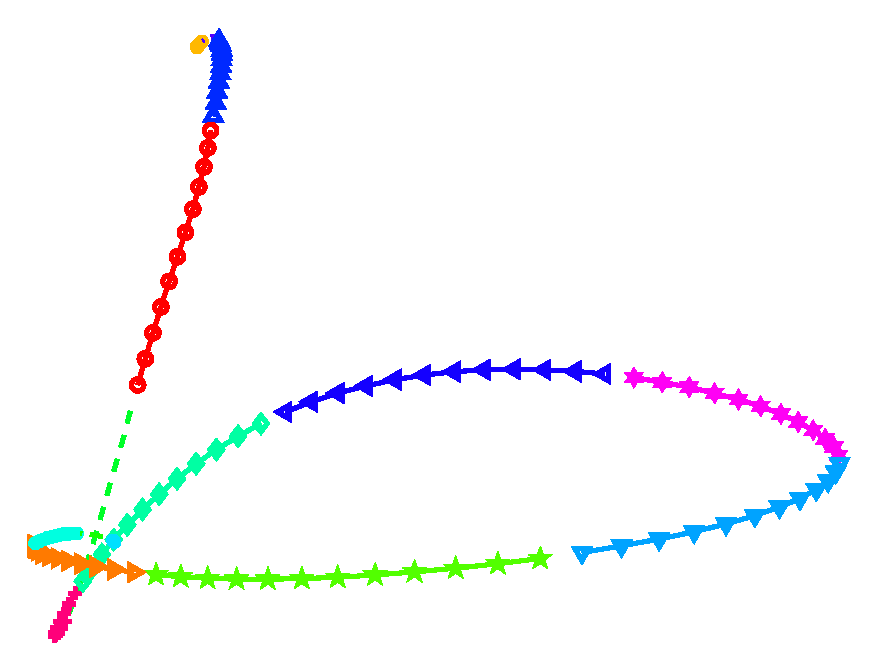
\includegraphics[width=.3\columnwidth]{./Graphic/Pic_words_forSystemSection/user_2_bphmn_2_at_3th_component.eps}}
&{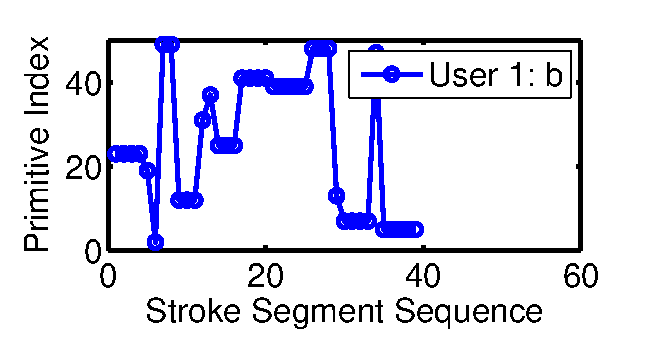
\includegraphics[width=.55\columnwidth]{./Graphic/Pic_words_forSystemSection/user1_b.eps}}  
&{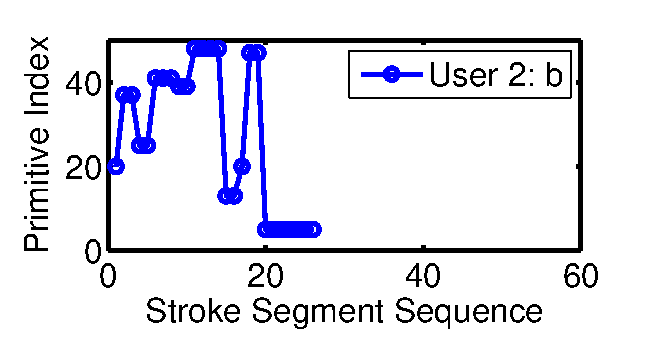
\includegraphics[width=.55\columnwidth]{./Graphic/Pic_words_forSystemSection/user2_b.eps}} &{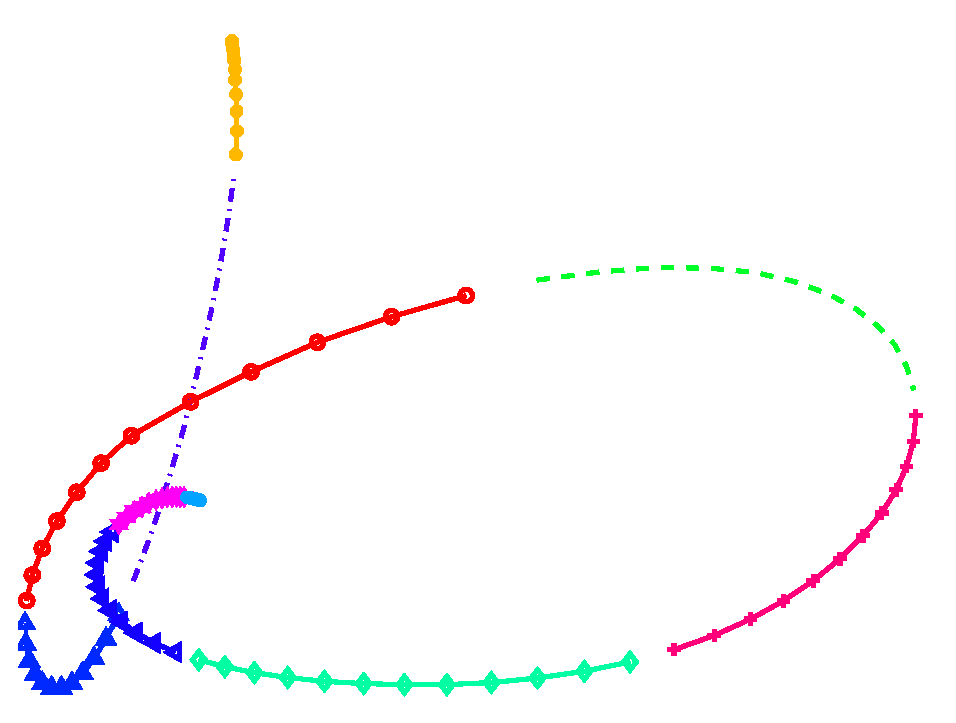
\includegraphics[width=.3\columnwidth]{./Graphic/Pic_words_forSystemSection/user_1_bphmn_2_at_5th_component.eps}} 

\\ \hline %\vspace{1mm}

 %LP.pdf
{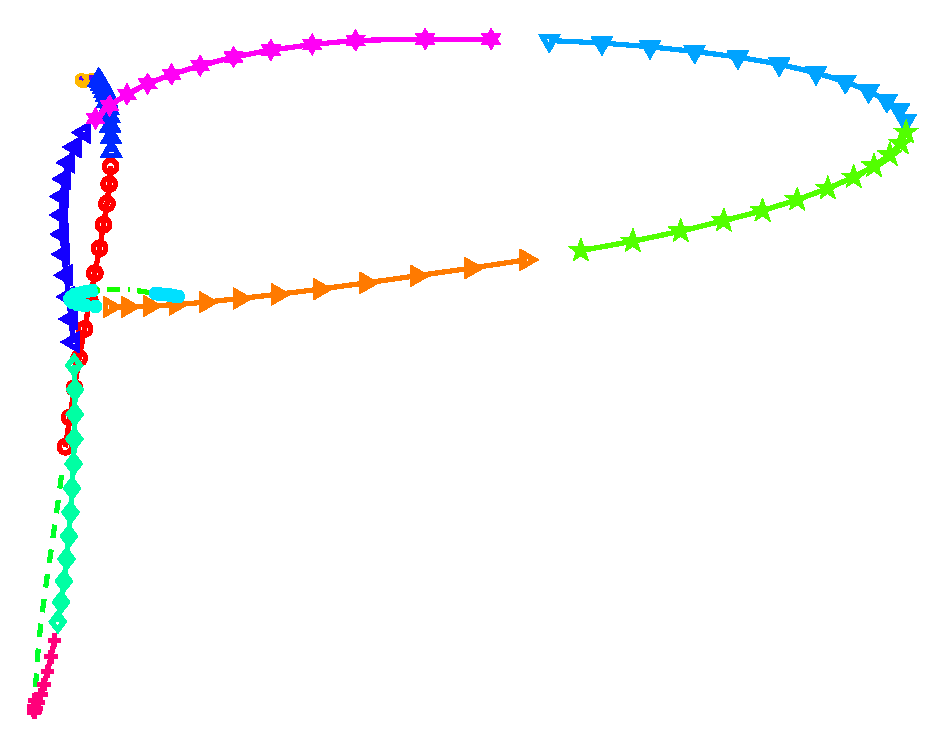
\includegraphics[width=.3\columnwidth]{./Graphic/Pic_words_forSystemSection/user_2_bphmn_2_at_4th_component.eps} }
&{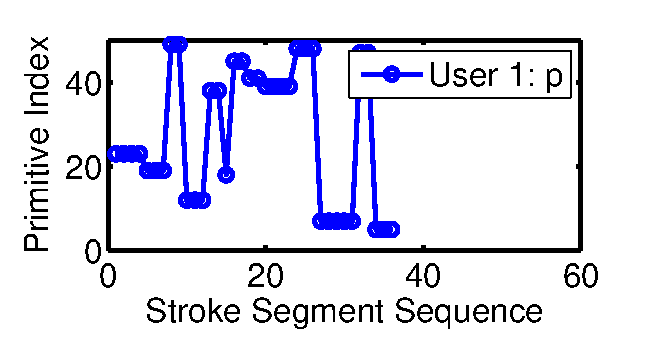
\includegraphics[width=.55\columnwidth]{./Graphic/Pic_words_forSystemSection/user1_p.eps} }%LP.pdf
&{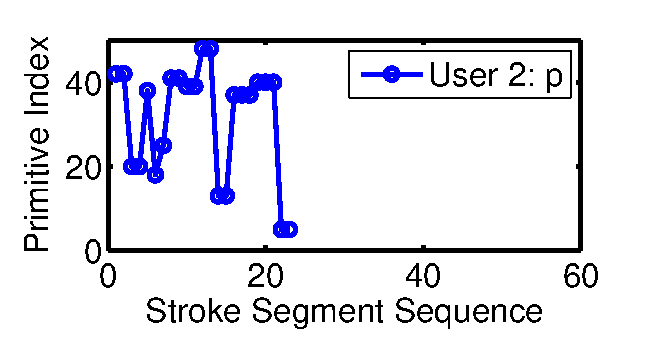
\includegraphics[width=.55\columnwidth]{./Graphic/Pic_words_forSystemSection/user2_p.eps}}
&{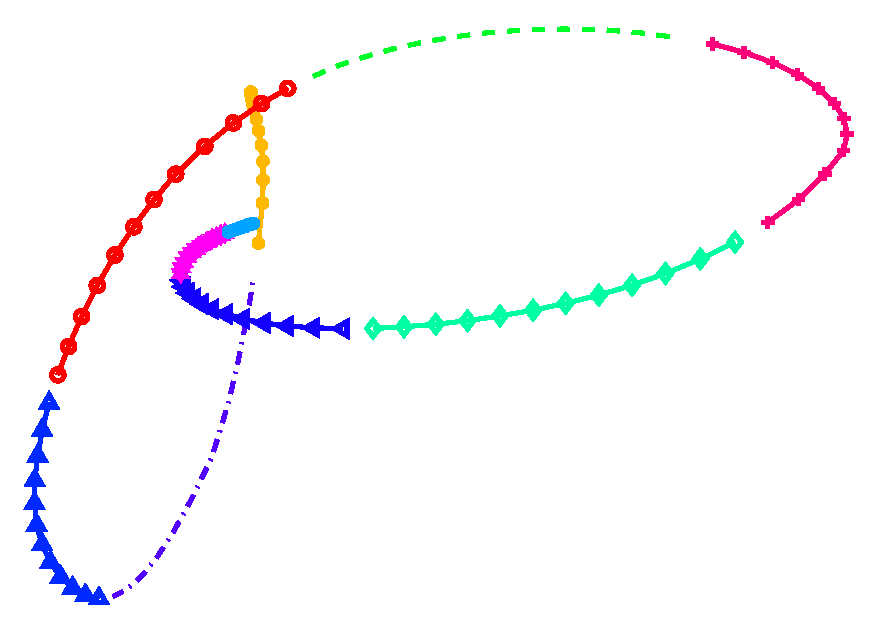
\includegraphics[width=.3\columnwidth]{./Graphic/Pic_words_forSystemSection/user_1_bphmn_2_at_8th_component.eps}} 
 \\ \hline 
 %\hline 
%
%
%% 
%%{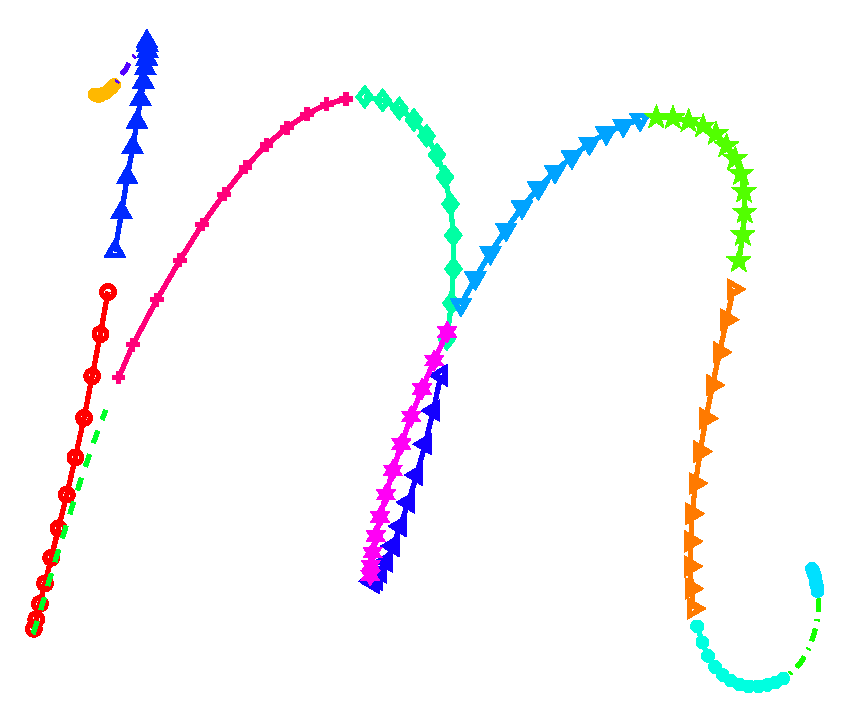
\includegraphics[width=.2\columnwidth]{./Graphic/Pic_words_forSystemSection/user_2_bphmn_1_at_5th_component.eps}}
%%&{\includegraphics[width=.5\columnwidth]{./Graphic/Pic_words_forSystemSection/1_m.eps}} 
%%&{\includegraphics[width=.5\columnwidth]{./Graphic/Pic_words_forSystemSection/2_m.eps}}  &{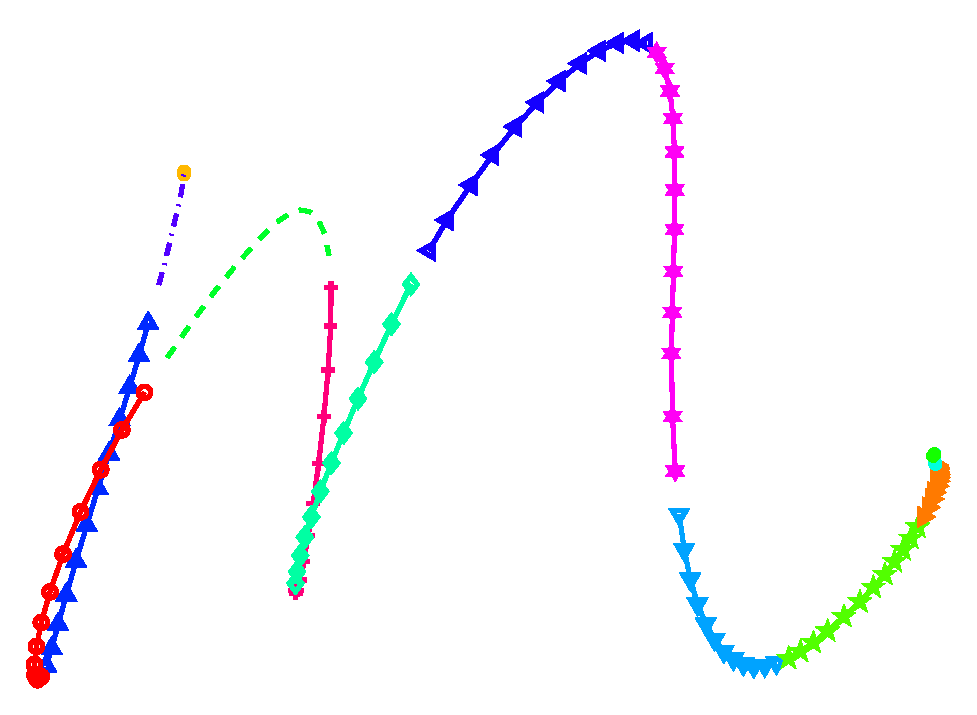
\includegraphics[width=.2\columnwidth]{./Graphic/Pic_words_forSystemSection/user_1_bphmn_1_at_8th_component.eps}} \\  \hline %\vspace{1mm}
%
%{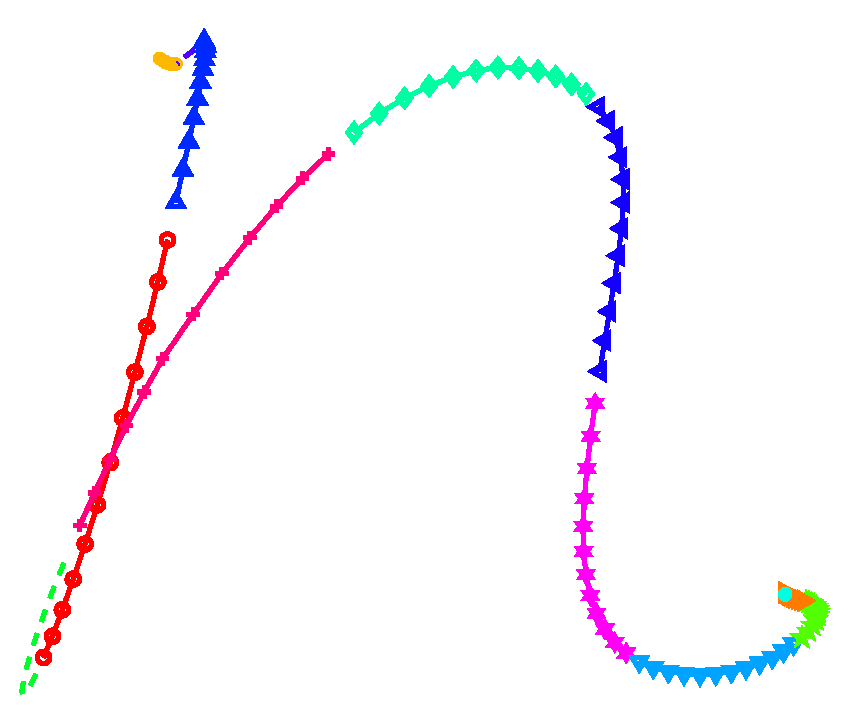
\includegraphics[width=.2\columnwidth]{./Graphic/Pic_words_forSystemSection/user_2_bphmn_1_at_6th_component.eps} } 
%&{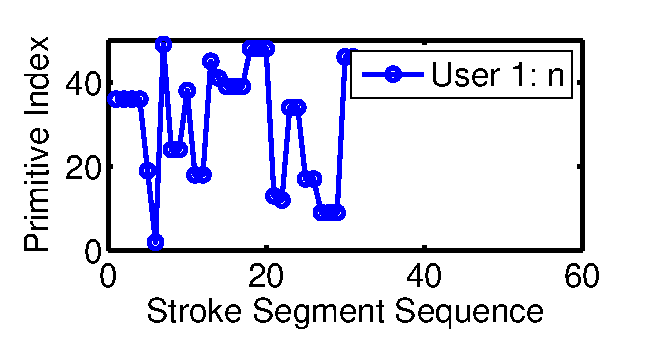
\includegraphics[width=.5\columnwidth]{./Graphic/Pic_words_forSystemSection/user1_n.eps}}
%&{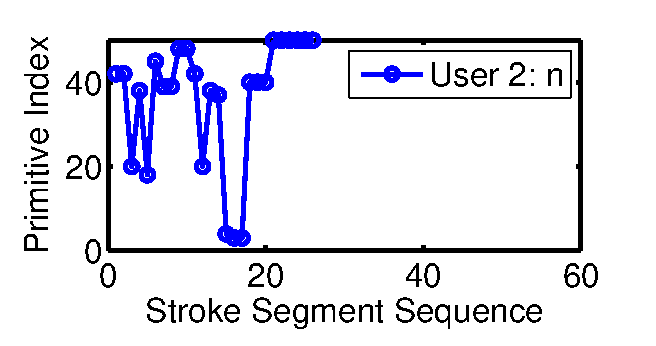
\includegraphics[width=.5\columnwidth]{./Graphic/Pic_words_forSystemSection/user2_n.eps}} 
%&{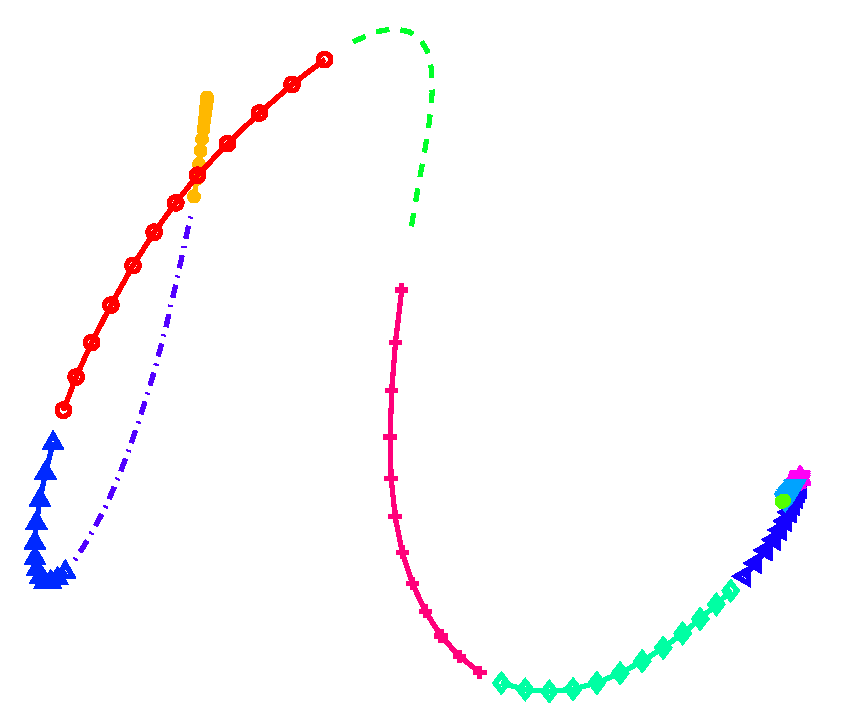
\includegraphics[width=.2\columnwidth]{./Graphic/Pic_words_forSystemSection/user_1_bphmn_1_at_9th_component.eps}} \\ \hline %\vspace{1mm}
%
%{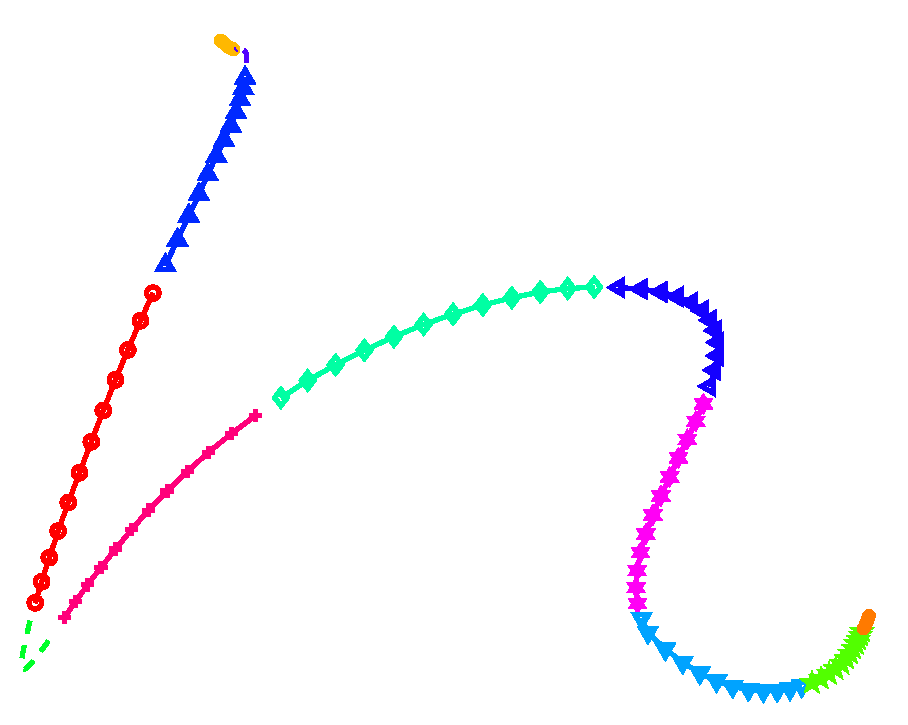
\includegraphics[width=.2\columnwidth]{./Graphic/Pic_words_forSystemSection/user_2_bphmn_1_at_10th_component.eps} }
%&{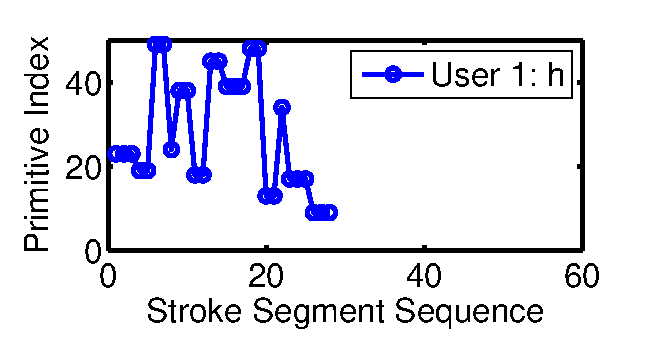
\includegraphics[width=.5\columnwidth]{./Graphic/Pic_words_forSystemSection/user1_h.eps}}
%&{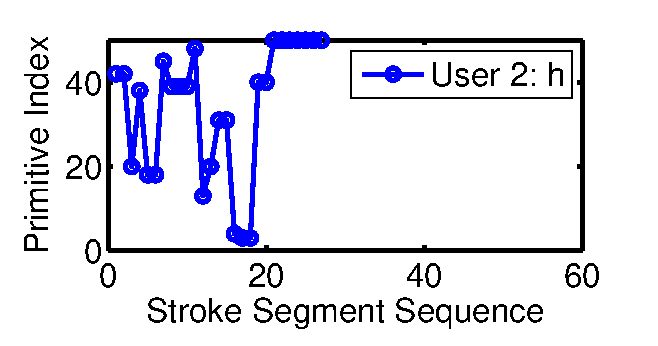
\includegraphics[width=.5\columnwidth]{./Graphic/Pic_words_forSystemSection/user2_h.eps}}  
%&{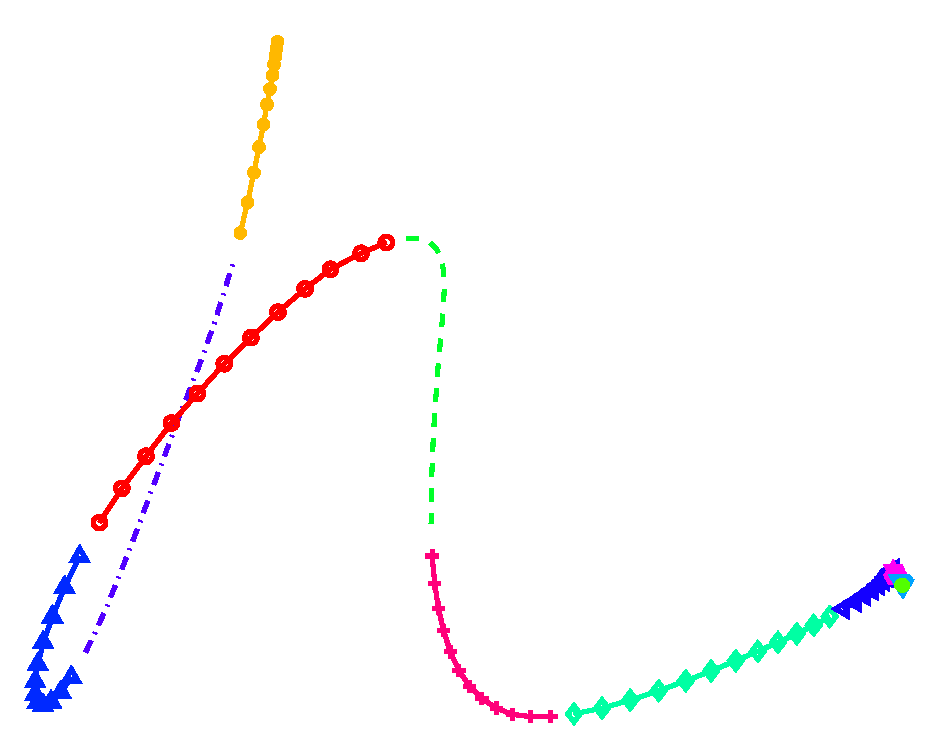
\includegraphics[width=.2\columnwidth]{./Graphic/Pic_words_forSystemSection/user_1_bphmn_1_at_4th_component.eps}} 
%\\ \hline%LP.pdf

\end{tabular}
\caption{{\jing{An illustration that characters written by the same user exhibit similarity while the ones by different users exhibit difference. We use 50 types of stroke segments (i.e., primitives) that consists of 12 continuous frames for illustration. The motion trajectories are divided into stroke segments, and the plots show the primitive-index ($y$-axis) change over time ($x$-axis). Plots with similar profiles represent the similarities of the handwriting style. 
Stroke segments (denoted by different colors on the characters) of \texttt{b} and \texttt{p} from the same user (either User 1 or User 2) show similar patterns, i.e., similar sequences of primitive indices, but the stroke segment sequences from the different users of the same letter (e.g.,  \texttt{b} or \texttt{p}) show distinguished patterns.
%Stroke segments (denoted by different colors on the characters) of `b' and `p' from the same user (either User 1 or User 2) show similar patterns in sequence donated by primitive indices, but the stroke segment sequences from the different users of the same letter `b' behave differently. %The observations also hold for `n' and `h'. 
}
}\vspace{-4mm}}\label{fig:bphmn}
%\end{minipage}
\end{figure*}



\subsection{Related Work}
\label{sec:related}
 
Challenge-response protocols are widely used for user verification over insecure channels. Randomly generatedchallenges and encrypted or hashed responses make the protocols resilient to replay attacks~\cite{Securityforcomputernetworks} and dictionary attacks~\cite{Bellovin92encryptedkey}. %Besides using secret keys to create response,  
O$'$Gorman \textit{et al.}, without experimental analysis, briefly suggested to create challenge-response protocols with biometrics~\cite{Gorman2003ComparingPasswords}, including speaker verification, keyboard dynamics.  %, and handwriting verification.  %Fuji \textit{et al.} also proposed to use voice to construct  a challenge response method without experiments~\cite{FujiiT13voice}. 
Johnson \textit{et al.}~\cite{johnson2013SPIE} proposed to use voice to construct a challenge response method that can verify users without breaching privacy. Their protocol uses encrypted feature vectors from real users and chaff ones from random people to create a hidden challenge that can only be recognized by the real users. Our work also uses biometrics, but our system utilizes motion instead of voice and can work in a noisy environment. %The basic idea is to let a server store an encrypted real feature vector derived from a user's voice and a chaff feature vector from a random people. Then the server encodes the challenge by mixing the real feature vectors and chaff ones. Because the users can correctly encrypt and identify the real feature vectors, they can recover the challenge and send it back. Our work also utilize biometrics

%However, they may not secure under dictionary attacks. Bellovin and Merritt improved the protocol by sharing common password to against dictionary attacks~\cite{Bellovin92encryptedkey}. O$'$Gorman suggested possible challenge-response protocols that combined with biometrics~\cite{Gorman2003ComparingPasswords}. Physical biometrics that contains stable personal information can response with random challenge and the collected biometric data, encrypt or not. However, the physical biometrics are limited and contains privacy personal information. Behavior biometrics are personal information hidden in human behavior.% (e.g., speaking, handwriting and typing). 
%For instance, the challenges of using voice to authenticate a user are random contents that are vocable. The responses are the corresponding voice data collected from the user. 
%Later, Fuji and Johnson utilize the voice verification to authenticate a user as part of a challenge-response method~\cite{FujiiT13voice,johnson2013SPIE}. However, the voice applications require quiet environment such that is not suitable for applications in public area. In addition, it is not applicable for continuous authentication if there are more than one person speaking.  To avoid these limitations, We applied a motion based biometric to challenge-response protocol to verify a user.
%, handwriting captured by depth sensors, 
 

%Biometric authentication is based on the unique physical characteristics of the human body. Biometric is limited and have privacy problem, 

%In biometrics, challenge response is the term used to describe the method by which the identification of a person is detected based on voluntary or involuntary responses. Challenge response is a type of biometric system security.





%\subsection{User Re-Authentication and Authentication}


%A typical re-authentication scheme  verifies a user continuously/periodically. 
%In 1985, using user behaviors for passive re-authentication was first proposed by Denning \emph{et al.}, whereby a statistical anomaly detector observes behavior on a monitored computer
%system and adaptively learns what is normal for subjects. Along the similar line, Szymanski~\emph{et al.} \cite{CoullBSB03} detect abnormal events by checking the inputs from command line using a bioinformatics approach. 


Recently, gestures embedded in the usage patterns of traditional I/O devices (e.g., keystroke dynamics~\cite{Revett:springerlink:10,Monrose:CCS99} and mouse movements, or clicks~\cite{Ahmed:TPDS07,Jorgensen11mouse}) and new input devices (e.g., wearable accelerometer sensors~\cite{Gafurov2007},  smart phones~\cite{Uell:CCS13, Derawi:2013} and multi-touch screens~\cite{SaeBaeCHI2012,Sherman:2014} ) can capture different types of gestures for authentication purpose. %. "Secret shakes" is used as a complementary authentication for traditional RFID card, shown in Google pattern~\cite{kohno2014radio}. 
%With the advances in multi-touch screens for smartphones and tablets, %how fingers operate touch screens has been used for authentication / 
%gestures of multi-touch (e.g., gestures using multiple fingers at the same time) are studied for authentication. Sae-Bae~\etal  { extracted} behavior-based biometrics from five-finger gestures and obtained a 90\% accuracy~\cite{SaeBaeCHI2012}, and Sherman~\etal { studied} the security and memorability on these free form gestures, which are not limited to single or multiple touches~\cite{Sherman:2014}. 
%Instead of pure finger gestures, several work proposed to combine other information with gestures. Zhao~\etal~\cite{USENIX2013Win8} analyzed finger gestures for authentication as users draw gestures on the touch screens with pictures displayed as background. % gesture authentication on Mirosoft Windows 8 touch screen and the designed attacks cracked a considerable portion of collected picture passwords under different settings~\cite{USENIX2013Win8}. 
%Uellenbeck~\etal { studied} the security performance of android system with an unlock pattern called Pass-Go scheme of $3\times 3$ grid size~\cite{Uell:CCS13}. De LucA~\etal~ combined a gesture and how the gesture was entered, and then evaluated the authentication performance~\cite{DeLuca:2012}.
%\$1, \$N, and \$P stroke recognizers developed by Wobbrock~\etal shows that the 2D gestures on the touch screen are possible to be used as a secret to authenticate users. Re-authentication for smart phones with gestures captured during daily usage are studied in~\cite{LiZX:NDSS13}. 
Our work also try to utilize gestures that are embedded in the usage patterns of input devices. However, none of the prior work studied the gestures associated with the emerging depth sensors, nor can they serve as a basis to construct challenge-response authentication.


%  gestures~\cite{Kubota:ISPACS06,Liu:2009MobiHCI,Shahzad:mobiCom13} and finger movements~\cite{TianQXW13:NDSS13}, % were also analyzed as authentication methods. 
%and touching gestures on the smart phone~\cite{LiZX:NDSS13}.

%From the other side of the fence, research has shown some of the behavior biometrics can be imitated. For instance, Serwadda~\etal~\cite{Serwadda:CCS13} show that a simple ``Lego'' robot can generate forgeries that achieve alarmingly high 
%penetration rates against touch-based authentication systems. Along the same line, work has shown that typing patterns of individuals can be imitated~\cite{Tey:NDSS13} as well.  Motivated by these imitation attacks, we aim at finding a biometrics that relies on motion-rich behaviors that can be more difficult to imitate. 

Authentication based on depth sensors has been studied on Microsoft Kinect~\cite{GaitKinectMS,Hayashi2014:WMU} and Leap Motion~\cite{Aslan14:LeapMidAirGesture, ICDAR15:OnlineHandwriting}.
% for instance, the user verification of two gestures that performed under three different device positions~\cite{Aslan14:LeapMidAirGesture}, the user identification based on hand shape information~\cite{Bernardos2015:LeapHandIdentify}, and character recognition~\cite{ICDAR15:OnlineHandwriting}. 
Using motion sensors to capture in-air handwriting for authenticatioin was first proposed to enhance text-base passwords~\cite{TianQXW13:NDSS13}. Then, Nigam~\etal ~proposed a recognition system based on fusion data of signatures from a Leap Motion sensor and face images from a camera~\cite{Nigam15:LeapSigVeri}. They both combine the writing content with the behavioral biometrics, and thus requires to write the same content for authentication.  
Our work is different because we try to harvest the writing style in the 3D-handwriting and do not depend on writing content. Thus, our work represents a harder problem and requires to utilize extra sophisticated features. 


Research on handwriting style has been used for identifying the person who wrote a document or determining whether multiple documents are written by the same person. \jing{Handwritings could be obtained offline (i.e., scanned images of handwriting~\cite{Bulacu:2003:EdgeBasedDirectional}), online by a digitizing tablet~\cite{Guru:PAM09}, or in the 3D space~\cite{TianQXW13:NDSS13}.
}
\jing{
Traditionally, handwriting styles mostly focus on off-line handwritings and features extraction include two classes: textural features (e.g., directionally and curvature of patterns in handwritten images), or allographs extracted from local handwritten patterns (i.e., shapes~\cite{Schomaker:2008}).
To extract handwriting styles, feature study techniques fall into two categories: statistical- and codebook- based feature extraction. For statictical method, Bulacu~\etal ~proposed edge based directional probability distributions as features~\cite{Bulacu:2003:EdgeBasedDirectional}. Schomaker~\etal ~proposed joint probability distribution of angle combination of two `hinged' edge fragments~\cite{Bulacu2003} and extended by~\cite{ICPR-2014-HeS}.
The codebook-based features are derived from Bags of (Visual) Words from computer vision community~\cite{Li:2005:BHM}. \textit{Primitives} in the codebook (i.e.,~\textit{vocabulary}) are local elements that extracted from writing data. Then a histogram of primitives refers from the codebook as characteristic for a user~\cite{Bulacu07text-independentwriter}. 
%Based on these, varies handwriting style features are derived. Newell~\etal used oriented Basic Image Features (oBIF) as their descriptors and enhanced textural based approch by a deviation encoding to provide a more informative encoding method~\cite{Newell:2014:OrientedBasicImageFeatures}. To better utilize the edge information, 
  Schomaker~\etal ~used the connected-component contours as the basic elements to capture features of the pen-tip trajectory~\cite{schomaker2004automatic} and then extened to ink-blob shapes~\cite{Bulacu07text-independentwriter}. These methods do not necessary work well in our problem because our handwriting is dynamic and contain temporal information (e.g., speed).
  
%  Recently, He~\etal extracted a Polar Stroke Descriptor that expresses the configuration of the entire stroke relative to the reference point in handwritten documents~\cite{He:ICDAR15:PolarStroke}. Singh~\etal used a more effective the subtractive clustering algorithm which does not rely on the initial choice of seed points (k-means or fuzzy c-means)~\cite{ICDAR2015:Singh}.
  
  
   %Jayanthi~\etal did texture analysis based on feature extracted from gray-level co-occurrence matrix of scanned image, which provided measure of the joint probability occurrence of the specified pixel pairs. 
}
%Gordo~\etc studied on handwritten musical scores with Bag of Visual Words framework. each handwriting style is modeled by a number of histogram-valued data computed for all the features in the feature set



On-line handwritings (e.g., handwriting recorded by a tablet) contain temporal information such as the velocity of the pen movements. For content-dependent application, 2D online handwritings are widely used for signature verification~\cite{Guru:PAM09}. For content-independent applications, the writing style analysis is applied in writer identification. Liwicki~\etal ~presented an on-line writer identification system for smart meeting rooms, used features at point (i.e., frame) level and stroke level extracted from text line~\cite{Liwicki2006:onlineSmartMeeting}.
Namboodiri~\etal ~used low level shape-based features and Li~\etal ~used stroke level at probility distribution~\cite{Li2007:StrokeProbabilityDistribution} and then extended to use temporal sequence codes for speed and pressure changes and shape codes for direction~\cite{conf/icdar/LiT09}. These work analyzed handwriting in 2D space and ours focused on 3D, which we believe introduces additional challenges due to the un-intended issues in the 3D space. In addition, existing writer identification methods used a large amount of testing text for testing, and are not suitable for authentication where userability is the key. For instance,~\cite{Liwicki2006:onlineSmartMeeting} used 80 words for a single test and~\cite{conf/icdar/LiT09} used one paragraph, about 40 Chinese and/or English characters, for a single test.
  
Compared to 2D handwriting, 3D handwriting style modeling is challenging, as trajectories are continuously recorded in 3D space, which results in no obvious stroke information or pen-up/down moments. In addition, the touch free input method provides less feedback while writing in-air and thus may result in inconsistency between trials. \jingjuly {?? To address it, we utilize both spatial and temporal information of the in-air writing recordings, adopt the concept of the stroke segment, and extract a vocabulary for writing-style-element representation. Instead of only using histograms of primitives, we introduce a co-occurrence matrix that quantifies the transition information between adjacent stroke segments, and our results show that the co-occurrence matrix method can achieve a better performance than histogram-based methods in our systems.
}



In particular, \CiT asks a user to write the content the system provides (the Challenge), and \CiT has to checks if the input content is the same as the system expected. We call this step as \texttt{content matching}.
Several literatures can be utilized for the content matching. 
For instance, \CiT can utilize online handwriting recognition that has been studied in pattern recognition community for a long time,  or similarity comparison based on handwriting recognition. Online handwriting recognition can achieve an accuracy of more than 85\% on pure cursive writings or 95\% on others ~\cite{Tappert90, LeeV12Cursive,Madhvanath2012,Plamondon2000Review}, while similarity comparison can achieve a higher accuracy, since it does not require the specific recognition of each letter, but a confidence score that shows similarities between two data. Furthermore, recent study~\cite{ICDAR15:OnlineHandwriting} achieved a recognition accuracy of 97.59\% for in-air English character recognition, with data from two depth sensors, Kinect and Leap Motion Controller. \jingjuly{ These methods could be applied to the content checking step of the challenge-response mechanism.

}




\section{\texttt{\CiT} System Overview}\label{sec:overview}



\begin{figure*}[b]
\vspace{-4mm}
\centering 	
 		{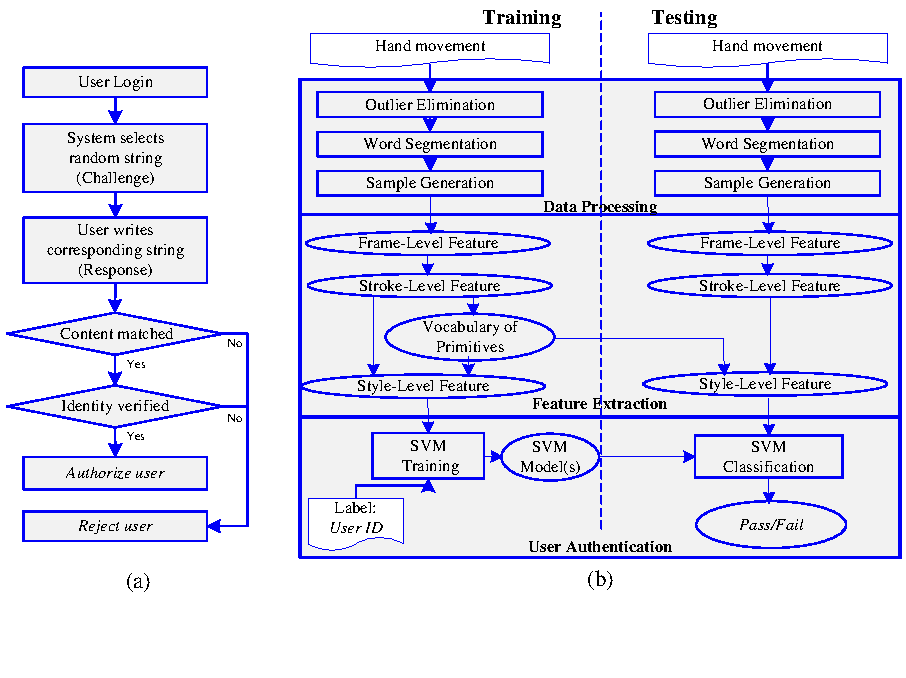
\includegraphics[width=2.0\columnwidth]{./Graphic/SystemFlow/SystemFlow_all_ccs_2017_style.pdf}}
\vspace{-18mm}
  \caption{\jing{(a) Flow chart of \CiT system. 
  (b) Flow chart of identity matching. 
  Details of the 3-Level feature extraction are shown in Figure~\ref{fig:featureFlow}.}
  \vspace{-3mm}
  }
  \label{fig:sysFlow}
\end{figure*}

\subsection{{Why does \CiT work?}}
%\subsection{Characterize Handwriting Styles} 

The \CiT system consists of two steps: verifying whether what a user writes matches what is asked for, and verifies the identity of the user. \jingap{
The first step is not the focus of this paper and can be accomplished by utilizing the prior work explained in Section~\ref{sec:related}.  
In particular, the user writes the content that the system provides (the Challenge). After receiving the input from the user (the Response), the system checks if the input content is the same as the system expected. As such, an attacker cannot simply `replay' handwriting performed in the past by a legitimate user. Based on the assumption that the replay attack would not be an issue for \CiT, 
}
%rely on existing technologies~\cite{ICDAR15:OnlineHandwriting,LeeV12Cursive,Madhvanath2012,Plamondon2000Review}, 
 we focus on the second step: how to verify users based on their handwriting styles, i.e., based on \textit{how} they write instead of \textit{what} they write. The challenges are to correctly recognize a user even if he/she writes different contents, and to distinguish users even if they write the same content. The difficulties stem from the possibility of handwriting variation (especially in writing different contents) of the same user and occasional handwriting similarity (especially in writing the same content) between different users.  The key to overcome the challenges is to characterize handwriting styles effectively and efficiently. 

\emph{Stroke Segments for Effective Modeling.} The model characterizing handwriting styles has to be content-independent. A naive approach could be to extract fingertip trajectories that represent each individual character and then to group the ones of the same characters for further comparison. However, such a method may be overkill, as the handwriting in the 3D space is difficult to be delimited precisely, as shown in \figref{fig:dataWords3user}. 
Although content recognition is possible, perfectly delimiting the fingertip trajectory of each letter is challenging. To avoid the burden of extracting individual symbols, we choose to characterize handwriting styles 
by short-length continuous trajectories, which are analogous to strokes~\cite{Component94,word-seg-stroke}. In practice, it is difficult to accurately divide a handwriting trajectory into meaningful strokes with variable lengths. We simply divide fingertip trajectories into a set of short, fixed-length \emph{stroke segments}. To reduce the impact of the starting point on a trajectory for stroke segment partition, we apply a temporal-sliding window over the fingertip trajectory for constructing stroke segment, and the constructed stroke segments can be partially overlapped.


Stroke segments can be considered as the basic building blocks that compose symbols. Although the underlying content in fingertip trajectories may be different, some characters may share similar stroke segments. Thus, the two fingertip trajectories created by the same user when writing different sets of words could contain a large percentage of the similar stroke segments. The stroke segments belonging to different users typically show little similarity.  For instance,  as shown in \figref{fig:bphmn}, the letters \texttt{b} and \texttt{p} have similar composition.
%, so do the letters `n' and `h'.  
Some stroke segments (denoted by different colors on the characters) of \texttt{b} and \texttt{p} from the same user show similarity, but the Stroke segments of User 1 are different from the ones of User 2. Thus, it is imaginable that the trajectories of the word \texttt{`bob'} and \texttt{`pop'} from the same user may have many similar stroke segments, but the ones from different users may share few similar stroke segments.


\emph{Vocabulary for Improving Efficiency.}
We define a \textit{frame} on a trajectory as a fingertip position, and consider the associated coordinates and kinematic features at each frame: \textit{frame-level features}. To compare the similarity between stroke segments, we can concatenate the frame-level features of all frames of a stroke segment to form \textit{stroke segment-level features}. Then,
we can combine all the stroke segment-level features of a trajectory sample to construct one \textit{style-level feature}, which is the unit to represent the handwriting style.  However, simply combining all the stroke segment-level features will lead to high-dimensional vectors. % and irregularized feature vectors.
To address this issue, we can define a stroke segment vocabulary that best represents the collection of stroke segments of all the enrolled users. The vocabulary consists of a set of primitives corresponding to typical stroke segments of those users, and each primitive will be assigned a unique index. The creation of a vocabulary can be conducted during the training phase. During the testing stage, each stroke segment is assigned the index of its nearest primitive. This way we reduce each high-dimensional stroke segment-level features to an integer index. 


Finally, to compare the similarity between handwriting styles of multiple samples, we perform statistical analysis to achieve content-independence.  Specifically, we obtain statistics on the stroke segment indices within a trajectory sample for constructing a low-dimensional feature for a sample. \jingap{Instead of using the histogram or probability density functions (PDFs) of the individual stroke segment indices~\cite{He:ICDAR15:PolarStroke, 
Bulacu07text-independentwriter, Li2007:StrokeProbabilityDistribution}}, we examine the temporal transition between stroke segments. The intuition is that a user may tend to write the same sequence of stroke segments, and such a sequence may be essential to represent handwriting styles. Concretely, we construct a co-occurrence matrix that counts the number of occurrences of each possible stroke segment (index) transition between temporally adjacent stroke segment pairs. This co-occurrence matrix reflects the distribution of the temporal stroke segment transition and we reshape it into a vector as a feature vector of a sample.




\begin{figure}[!b]
\vspace{-8mm}
\centering
\begin{tabular}{c}
{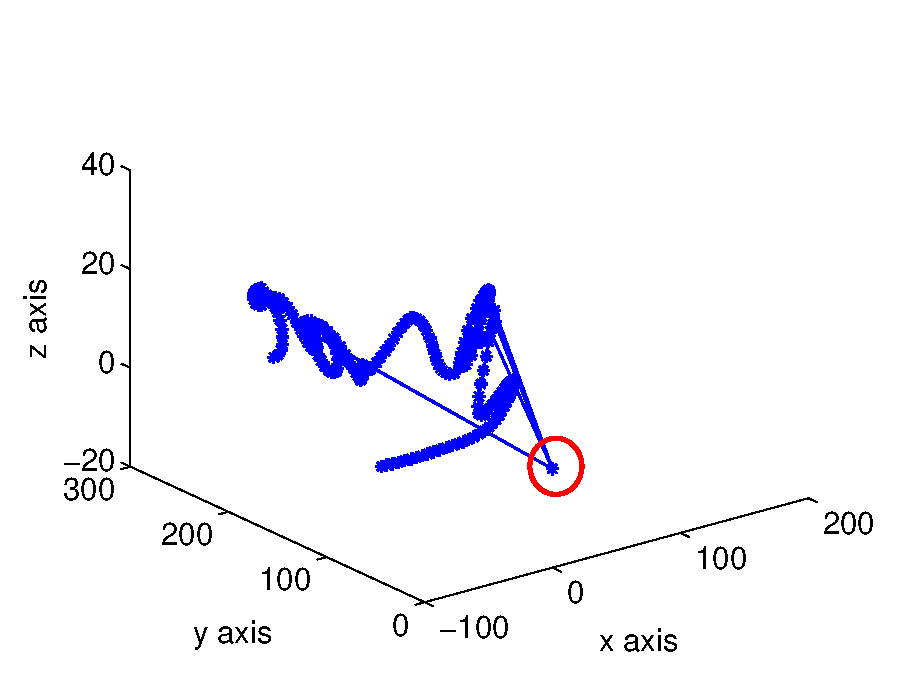
\includegraphics[width=0.65\columnwidth]{./Graphic/noise/noise_1.eps}} 
% &
%{\includegraphics[width=0.53\columnwidth]{./Graphic/noise/noise_2.eps}}  &
%{\includegraphics[width=0.53\columnwidth]{./Graphic/noise/noise_3.eps}}
\end{tabular}
\vspace{-2mm}
\caption{An illustration of the outliers in Leap Motion data. The red circles highlight the frames with outliers.}
\label{fig:noises}
\end{figure}




Continue with the example in \figref{fig:bphmn}, $50$ primitives were derived to form a vocabulary for illustration. We observe that the similar letter sets (e.g., \texttt{b} and \texttt{p}) written by the same user contain similar stroke segment indices and transition pattern of stroke segment indices, while the stroke segment sequences of the same letter (e.g., \texttt{b} or \texttt{p}) written by different users share few similarities.  
%In particular, we notice that the index sequence of character `b' and `p' written by the same subject show strong similarity, while the same characters written by different users exhibit difference. 
This example encourages us to study the effectiveness of using vocabulary and transition between stroke segments to model the handwriting style. 

\subsection{{How does \CiT work?}}
%\subsection{System Overview}



The \CiT system consists of a Leap Motion for capturing fingertip movements in the 3D space, computing and storage units for challenge-response processing and identity authentication. \figref{fig:sysFlow}(a) shows the flow chart of the challenge-response authentication. 

The \CiT authentication process consists of two phases: enrollment and testing. During an enrollment, the system will capture the initial handwriting and create an account for a user. These handwriting inputs will be used for training. In a testing phase, the system first select a random string. After capturing the user's writing movements, the system first performs a content check, i.e., verifying whether what a user writes matches the random string, and then tests the user's identity.  \figref{fig:sysFlow} illustrates a detailed flow chart of identity matching. 

\jingap{
\emph{Content Matching.} 
The focus of this paper is to study the biometrics built in handwriting motions instead of the content check, because several literatures can achieve the content check, as shown in Section~\ref{sec:related}. Therefore, we do not include the technique details of this part in the paper. } 

%Spatial Features : Trajectory formation Normalization to  fixed center of gravity for the system.

%In addition, since our handwriting data is written in the air, we can project the 3D writings into its main plane (a 2D plane). 
%We briefly overview the biometric-related processes in this section and postpone the detailed discussion to Section~\ref{sec:data} and ~\ref{sec:feature}.  
%Note that our system can perform a content check to detect such scenarios, i.e., utilizing similarity comparison or content recognition using online handwritng recognition techniques~\cite{Tappert90}.  


\emph{Data Processing.} Both training and testing phases require data processing and feature extraction. The goal of data processing is to prepare the raw motion data captured by Leap Motion and generate a handwriting sample, which consists of a number of frames that represent the motion of the fingertip. 
The data processing will remove outliers and meaningless transition trajectories from the data,  as well as partition the handwriting trajectory into samples, on which the features can be calculated to represent the writing style. 


\emph{Feature Extraction.} After data processing, a \CiT system extracts three levels of features from each sample: frame-level features, stroke segment-level features, and style-level features. Level by level, the \CiT system is able to derive features that effectively and efficiently model the handwriting styles of users. 

\emph{SVM Training and Testing.}
In \figref{fig:sysFlow}, \CiT system uses the extracted style-level features for both classifier training and testing. The classifier has to achieve two goals: correctly authenticate a legitimate user and reject any impostors that are not part of the pool. %This maps to the scenario of teleconference, whereby the system tries to identify whether the comments are entered by one of the attendees or by an attacker. 









\section{Data Processing}
\label{sec:data}

Data processing constructs samples from raw data recorded by Leap Motion, and consists of \textit{outlier elimination}, \textit{word segmentation}, and \textit{sample generation}. 



%%%
%%\begin{figure}[t]
%%%\small
%%\centering
%%\vspace{2mm}
%%\begin{tabular}{|c||c|c|c|c|c|c|}
%%\hline %\hline
%%Sample & \multicolumn{4}{c|}{s1}  & \multicolumn{2}{c|}{s2} \\ \hline
%%\# Frames  &231   &169   &231   &149   &260   &144      \\
%%User 1
%%&{\includegraphics[width=0.07\columnwidth,totalheight=.018\textheight]{./Graphic/words_jing/1001_pdf.eps}}
%%&{\includegraphics[width=0.07\columnwidth,totalheight=.018\textheight]{./Graphic/words_jing/1002_pdf.eps}}
%%&{\includegraphics[width=0.07\columnwidth,totalheight=.018\textheight]{./Graphic/words_jing/1003_pdf.eps}}
%%&{\includegraphics[width=0.07\columnwidth,totalheight=.018\textheight]{./Graphic/words_jing/1004_pdf.eps}}
%%&{\includegraphics[width=0.07\columnwidth,totalheight=.018\textheight]{./Graphic/words_jing/1005_pdf.eps}}
%%&{\includegraphics[width=0.07\columnwidth,totalheight=.018\textheight]{./Graphic/words_jing/1007_pdf.eps}}\\ \hline \hline
%%
%%Sample   &\multicolumn{2}{c|}{s1} &\multicolumn{2}{c|}{s2} &\multicolumn{2}{c|}{s3}  \\ \hline
%%\# Frames &466  & 288   &430   &183   &512   &264       \\
%%User 2
%%&{\includegraphics[width=0.07\columnwidth,totalheight=.018\textheight]{./Graphic/words_meng/10001_pdf.eps}}
%%&{\includegraphics[width=0.07\columnwidth,totalheight=.018\textheight]{./Graphic/words_meng/10002_pdf.eps}}
%%&{\includegraphics[width=0.07\columnwidth,totalheight=.018\textheight]{./Graphic/words_meng/10003_pdf.eps}}
%%&{\includegraphics[width=0.07\columnwidth,totalheight=.018\textheight]{./Graphic/words_meng/10004_pdf.eps}}
%%&{\includegraphics[width=0.07\columnwidth,totalheight=.018\textheight]{./Graphic/words_meng/10005_pdf.eps}}
%%&{\includegraphics[width=0.07\columnwidth,totalheight=.018\textheight]{./Graphic/words_meng/10007_pdf.eps}}\\ \hline 
%%
%%\end{tabular}\vspace{-0mm}
%%\caption{An illustration of constructing samples from a group of words. { 
%%%The frame numbers and sample labels of each word segment are listed, and a
%%All the word segments with the same sample label (e.g., s1, s2) constitute a  sample. 
%%Given each sample length $L_s$ is no larger than 800 frames, $6$ words form different numbers of samples for Users 1 and 2.% , due to the different writing speeds.
%%} \vspace{0mm}}\label{fig:dataWords}
%%\end{figure}



\subsection{Leap Motion Data}
Leap Motion captures finger movements in a 3D space (as shown in \figref{fig:leap}):  the left-right motion will be recorded at the $x$-direction, the up-down motion at $y$-direction and the forward-backward motion at the $z$-direction. 
As a user raises his/her hands and uses one of the fingers to write,  a Leap Motion controller will capture information of up to 10 fingers (depending on their visibility). We extract the data of the foremost fingertip (i.e., the ones with the smallest $z$-value among all captured figures), and record a 11-dimensional vector with the information provided directly by Leap Motion (listed below) at time $t$ as a \textit{frame}.  
%\begin{inlinenum}
\begin{enumerate}
\setlength{\itemsep}{-0.5mm}
\item fingertip position,\quad -- $(p_x(t), p_y(t),p_z(t))$, 
\item fingertip velocity,\quad -- $(v_x(t), v_y(t),v_z(t))$, 
\item fingertip direction,\quad -- $(D_x(t), D_y(t),D_z(t))$, 
\item finger visible length and width,\quad -- $L_f(t)$ and $W_f(t)$. 
\end{enumerate}
%\end{inlinenum}
In addition, Leap Motion provides an ID number and a timestamp for each frame. The ID number of each frame for objects (e.g., fingers) is given as a positive number if at least one object is detected or becomes a negative number if no recognizable objects are detected. Thus, we utilize the ID numbers to check the validity of a frame and utilize timestamps to calculate the speed of handwriting. 
For each round of recording, Leap Motion will record a collection of  frames, by sequentially connecting all consecutive frames, we construct a raw handwriting trajectory.  



\begin{figure}[!t]
\vspace{-2mm}
\centering

\begin{tabular}{cc}
\subfigure[]
{\includegraphics[width=0.45\columnwidth]{./Graphic/Pic_words_forSystemSection/segmentation1.pdf}} 
\subfigure[]
{\includegraphics[width=.45\columnwidth]{./Graphic/pictures_seg/x-seg_1.eps}} 
%&\subfigure[]
%{\includegraphics[width=.6\columnwidth]{./Graphic/pictures_seg/y-seg.eps}} 
%&\subfigure[]
%{\includegraphics[width=.6\columnwidth]{./Graphic/pictures_seg/z-seg.eps}}
\end{tabular}
\begin{tabular}{ccc}

\begin{tabular}{c}
{\includegraphics[width=0.22\columnwidth]{./Graphic/Pic_words_forSystemSection/1_thWord.eps}}
\end{tabular}
\vspace{-0mm}
& 
\begin{tabular}{c}
{\includegraphics[width=0.22\columnwidth]{./Graphic/Pic_words_forSystemSection/2_thWord.eps}}
\end{tabular} 
\vspace{-0mm}
&
\begin{tabular}{c}
{\includegraphics[width=0.22\columnwidth, height = 0.2\columnwidth]{./Graphic/Pic_words_forSystemSection/3_thWord.eps}} 
\end{tabular}
\vspace{-0mm} 
\\ 
\multicolumn{3}{c}{(c)} 

\end{tabular}

\vspace{-2mm}
\caption{{ {An illustration of word segmentation. (a) what was recorded by the Leap Motion controller, which contains three words and transition trajectories connecting them. (b) word segmentation results on x-axis. The trajectories starting from a red square and ending at the next green square are the transition ones, which are removed to obtain word segments. (c) shows the separated words from the trajectory in (a). \jingap{Note that the subject draw the point before the lower part of the letter `i'.}
}}\vspace{-0mm}}
\label{fig:segmentation}
\end{figure}




\begin{figure*}[ht]
\vspace{2mm}
\small
\centering
\begin{tabular*}{0.8\paperwidth}{ @{\extracolsep{\fill}} |p{0.9cm}|c||c|c|c|c|c|c|c|c|c|c|}
\hline %\hline
\multirow{12}{*}{User 1} 
& Sample Label & \multicolumn{9}{c|}{s1}  & s2 \\ \cline{2-12}
& \# Frames  &231   &169   &231   &149   &260   &144   &179   &305   &220   &356\\
& %User 1
&{\includegraphics[width=0.07\columnwidth,totalheight=.018\textheight]{./Graphic/words_jing/1001_pdf.eps}}
&{\includegraphics[width=0.07\columnwidth,totalheight=.018\textheight]{./Graphic/words_jing/1002_pdf.eps}}
&{\includegraphics[width=0.07\columnwidth,totalheight=.018\textheight]{./Graphic/words_jing/1003_pdf.eps}}
&{\includegraphics[width=0.07\columnwidth,totalheight=.018\textheight]{./Graphic/words_jing/1004_pdf.eps}}
&{\includegraphics[width=0.07\columnwidth,totalheight=.018\textheight]{./Graphic/words_jing/1005_pdf.eps}}
&{\includegraphics[width=0.07\columnwidth,totalheight=.018\textheight]{./Graphic/words_jing/1007_pdf.eps}}
&{\includegraphics[width=0.07\columnwidth,totalheight=.018\textheight]{./Graphic/words_jing/1008_pdf.eps}}
&{\includegraphics[width=0.08\columnwidth,totalheight=.018\textheight]{./Graphic/words_jing/1010_pdf.eps}}
&{\includegraphics[width=0.08\columnwidth,totalheight=.018\textheight]{./Graphic/words_jing/1011_pdf.eps}}
&{\includegraphics[width=0.08\columnwidth,totalheight=.018\textheight]{./Graphic/words_jing/1012_pdf.eps}}\\ 
& & \texttt{when}   &\texttt{it}   &\texttt{comes}  & \texttt{to} &\texttt{play}   &\texttt{do}   &\texttt{not}   &\texttt{would}   &\texttt{other}   & \texttt{speaks}  \\
\cline{2-12}
& Sample Label & \multicolumn{8}{c|}{s2}  & \multicolumn{2}{c|}{s3}   \\ \cline{2-12}
& \# Frames  &184   &214   &221  & 139  & 226    &98   &137   &210    &269  & 227 \\
& %User 1
&{\includegraphics[width=0.07\columnwidth,totalheight=.018\textheight]{./Graphic/words_jing/1014_pdf.eps}}
&{\includegraphics[width=0.07\columnwidth,totalheight=.018\textheight]{./Graphic/words_jing/1015_pdf.eps}}
&{\includegraphics[width=0.07\columnwidth,totalheight=.018\textheight]{./Graphic/words_jing/1019_pdf.eps}}
&{\includegraphics[width=0.07\columnwidth,totalheight=.018\textheight]{./Graphic/words_jing/1020_pdf.eps}}
&{\includegraphics[width=0.08\columnwidth,totalheight=.018\textheight]{./Graphic/words_jing/1021_pdf.eps}}
&{\includegraphics[width=0.07\columnwidth,totalheight=.018\textheight]{./Graphic/words_jing/1026_pdf.eps}}
&{\includegraphics[width=0.07\columnwidth,totalheight=.018\textheight]{./Graphic/words_jing/1027_pdf.eps}}
&{\includegraphics[width=0.07\columnwidth,totalheight=.018\textheight]{./Graphic/words_jing/1032_pdf.eps}}
&{\includegraphics[width=0.07\columnwidth,totalheight=.018\textheight]{./Graphic/words_jing/1034_pdf.eps}}
&{\includegraphics[width=0.07\columnwidth,totalheight=.018\textheight]{./Graphic/words_jing/4027_pdf.eps}}\\ 
& & \texttt{but}   &\texttt{note}   &\texttt{much}  & \texttt{of} &\texttt{their}   &\texttt{or}   &\texttt{as}   &\texttt{much}   &\texttt{from}   & \texttt{told}  \\
\cline{2-12}
& Sample Label & \multicolumn{7}{c|}{s3} & \multicolumn{3}{c|}{\textbf{s4}}  \\ \cline{2-12}
&\# Frames &136  &155  &238   &233  & 188 &  223  & 245  & 145   &191  & 178 \\
& %User 1
&{\includegraphics[width=0.07\columnwidth,totalheight=.018\textheight]{./Graphic/words_jing/3011_pdf.eps}}
&{\includegraphics[width=0.07\columnwidth,totalheight=.018\textheight]{./Graphic/words_jing/3016_pdf.eps}}
&{\includegraphics[width=0.07\columnwidth,totalheight=.018\textheight]{./Graphic/words_jing/2003_pdf.eps}}
&{\includegraphics[width=0.07\columnwidth,totalheight=.018\textheight]{./Graphic/words_jing/2008_pdf.eps}}
&{\includegraphics[width=0.07\columnwidth,totalheight=.018\textheight]{./Graphic/words_jing/2014_pdf.eps}}
&{\includegraphics[width=0.07\columnwidth,totalheight=.018\textheight]{./Graphic/words_jing/2015_pdf.eps}}
&{\includegraphics[width=0.07\columnwidth,totalheight=.018\textheight]{./Graphic/words_jing/2018_pdf.eps}}
&{\includegraphics[width=0.07\columnwidth,totalheight=.018\textheight]{./Graphic/words_jing/2016_pdf.eps}}
&{\includegraphics[width=0.07\columnwidth,totalheight=.018\textheight]{./Graphic/words_jing/3001_pdf.eps}}
&{\includegraphics[width=0.08\columnwidth,totalheight=.018\textheight]{./Graphic/words_jing/3002_pdf.eps}}\\ 
& & \texttt{one}   &\texttt{her}   &\texttt{game}  & \texttt{have} &\texttt{out}   &\texttt{what}   &\texttt{that}   &\texttt{it}   &\texttt{last}   & \texttt{summer}  \\
\hline 
\hline

\multirow{12}{*}{User 2} 
& Sample Label  &\multicolumn{5}{c|}{s1} &\multicolumn{4}{c|}{s2} &s3  \\ \cline{2-12}
& \# Frames &466  & 288   &430   &183   &512   &264  & 345  & 627   &499   &713  \\ 
& %User 2 
&{\includegraphics[width=0.07\columnwidth,totalheight=.018\textheight]{./Graphic/words_meng/10001_pdf.eps}}
&{\includegraphics[width=0.07\columnwidth,totalheight=.018\textheight]{./Graphic/words_meng/10002_pdf.eps}}
&{\includegraphics[width=0.07\columnwidth,totalheight=.018\textheight]{./Graphic/words_meng/10003_pdf.eps}}
&{\includegraphics[width=0.07\columnwidth,totalheight=.018\textheight]{./Graphic/words_meng/10004_pdf.eps}}
&{\includegraphics[width=0.07\columnwidth,totalheight=.018\textheight]{./Graphic/words_meng/10005_pdf.eps}}
&{\includegraphics[width=0.07\columnwidth,totalheight=.018\textheight]{./Graphic/words_meng/10007_pdf.eps}}
&{\includegraphics[width=0.07\columnwidth,totalheight=.018\textheight]{./Graphic/words_meng/10008_pdf.eps}}
&{\includegraphics[width=0.08\columnwidth,totalheight=.018\textheight]{./Graphic/words_meng/10010_pdf.eps}}
&{\includegraphics[width=0.08\columnwidth,totalheight=.018\textheight]{./Graphic/words_meng/10011_pdf.eps}}
&{\includegraphics[width=0.08\columnwidth,totalheight=.018\textheight]{./Graphic/words_meng/10012_pdf.eps}}\\ 
& & \texttt{when}   &\texttt{it}   &\texttt{comes}  & \texttt{to} &\texttt{play}   &\texttt{do}   &\texttt{not}   &\texttt{would}   &\texttt{other}   & \texttt{speaks}  \\
\cline{2-12} 
& Sample Label &\multicolumn{3}{c|}{s3} &\multicolumn{6}{c|}{s4} & s5  \\  \cline{2-12}
& \# Frames &364   &384  & 481  & 259 &  498  & 220  & 162   &399  & 454 & 264 \\
& %User 2
&{\includegraphics[width=0.07\columnwidth,totalheight=.018\textheight]{./Graphic/words_meng/10014_pdf.eps}}
&{\includegraphics[width=0.07\columnwidth,totalheight=.018\textheight]{./Graphic/words_meng/10015_pdf.eps}}
&{\includegraphics[width=0.07\columnwidth,totalheight=.018\textheight]{./Graphic/words_meng/10019_pdf.eps}}
&{\includegraphics[width=0.07\columnwidth,totalheight=.018\textheight]{./Graphic/words_meng/10020_pdf.eps}}
&{\includegraphics[width=0.08\columnwidth,totalheight=.018\textheight]{./Graphic/words_meng/10021_pdf.eps}}
&{\includegraphics[width=0.07\columnwidth,totalheight=.018\textheight]{./Graphic/words_meng/10026_pdf.eps}}
&{\includegraphics[width=0.07\columnwidth,totalheight=.018\textheight]{./Graphic/words_meng/10027_pdf.eps}}
&{\includegraphics[width=0.07\columnwidth,totalheight=.018\textheight]{./Graphic/words_meng/10032_pdf.eps}}
&{\includegraphics[width=0.07\columnwidth,totalheight=.018\textheight]{./Graphic/words_meng/10034_pdf.eps}}
&{\includegraphics[width=0.07\columnwidth,totalheight=.018\textheight]{./Graphic/words_meng/40027_pdf.eps}} \\ 
& & \texttt{but}   &\texttt{note}   &\texttt{much}  & \texttt{of} &\texttt{their}   &\texttt{or}   &\texttt{as}   &\texttt{much}   &\texttt{from}   & \texttt{told} \\
\cline{2-12}
& Sample Label &\multicolumn{5}{c|}{s5}  &\multicolumn{5}{c|}{\textbf{s6}}  \\  \cline{2-12}
& \# Frames  & 210 &217   &488   &381   &243   &352  & 399  & 211   &370   &251 \\
& %User 2
&{\includegraphics[width=0.07\columnwidth,totalheight=.018\textheight]{./Graphic/words_meng/30011_pdf.eps}}
&{\includegraphics[width=0.07\columnwidth,totalheight=.018\textheight]{./Graphic/words_meng/30016_pdf.eps}}
&{\includegraphics[width=0.07\columnwidth,totalheight=.018\textheight]{./Graphic/words_meng/20003_pdf.eps}}
&{\includegraphics[width=0.07\columnwidth,totalheight=.018\textheight]{./Graphic/words_meng/20008_pdf.eps}}
&{\includegraphics[width=0.07\columnwidth,totalheight=.018\textheight]{./Graphic/words_meng/20014_pdf.eps}}
&{\includegraphics[width=0.07\columnwidth,totalheight=.018\textheight]{./Graphic/words_meng/20015_pdf.eps}}
&{\includegraphics[width=0.07\columnwidth,totalheight=.018\textheight]{./Graphic/words_meng/20018_pdf.eps}}
&{\includegraphics[width=0.07\columnwidth,totalheight=.018\textheight]{./Graphic/words_meng/20016_pdf.eps}}
&{\includegraphics[width=0.07\columnwidth,totalheight=.018\textheight]{./Graphic/words_meng/30001_pdf.eps}}
&{\includegraphics[width=0.08\columnwidth,totalheight=.018\textheight]{./Graphic/words_meng/30002_pdf.eps}} \\
& & \texttt{one}   &\texttt{her}   &\texttt{game}  & \texttt{have} &\texttt{out}   &\texttt{what}   &\texttt{that}   &\texttt{it}   &\texttt{last}   & \texttt{summer} 
\\  
\hline 

%%\end{tabular*}\vspace{-0mm}
%%\caption{An illustration of constructing samples out of a group of words. 
%%Each word segment's frame numbers and sample labels are listed, and all the word segments with the same sample label constitute a  sample. For each user, $20$ word segments can construct different numbers of samples due to the different writing speeds.
%%The frame numbers and sample labels of each word segment are listed, and all the word segments with the same sample label (e.g., s1, s2) constitute a  sample. 
%%Given each sample length $L_s$ is no larger than 2000 frames, $20$ words form different numbers of samples for Users 1 and 2, due to the different writing speeds.
%%}\label{fig:dataWords}
%%\end{figure*}

\end{tabular*}\vspace{-0mm}
\caption{\jing{An illustration of constructing samples from a group of words.  
%The frame numbers and sample labels of each word segment are listed, and a
All the word segments with the same sample label (e.g., s1, s2) constitute a  sample. 
Given the sample length $L_s$ that is no larger than 2000 frames, $30$ words form around 4 or 6 samples for Users 1 and 2, respectively, due to the different writing speeds.
} \vspace{0mm}}\label{fig:dataWords}
\end{figure*}




\subsection{Outlier Elimination}
% define different noise types
Noises caused by environment variation may affect the Leap Motion raw trajectories. In general, such noises lead to abrupt changes of the fingertip positions between adjacent frames, as shown in Figure~\ref{fig:noises}. 
Therefore, they are actually outliers. In general, we observe two types of outliers: (1) no fingertip is detected ($7.32\%$ amount of data), and (2) a fingertip is detected but at an unlikely position (less than $1\%$ amount of data). For no-detection cases, we examine the number of consecutive frames that do not contain detected fingertips. If the number is small, we perform spatial interpolation. If the number of noisy frames is large, we discard the noisy frames and divide the raw trajectory into two. 
Then we can perform the remaining data processing and feature extraction steps on each trajectory independently. 
For unlikely-position cases, we apply a temporal median filter to remove the outliers~\cite{SaltNoise}. 
At each frame, we examine a temporal window centered at this frame, search for the median of all values in this window,  and set the median as the new value of this frame. 
The median filter is applied not only on the $x$, $y$ and $z$ positions but also values on other dimensions. For both cases, our algorithm only removes the outliers and preserves the smoothness and continuity of the handwritings. 





%==================================================================



 \subsection{Word Segmentation}

The main goal of word segmentation is to identify the segments of the handwriting trajectories that contain useful information for recognizing handwriting styles. 
When writing on paper, we proceed from  left to right % and from the top to the bottom 
without text overwriting. % or connecting lines between words.
However, Leap Motion has limited writing space within which the hand motion can be captured -- after writing one or two words, a finger becomes out of the Leap Motion's field of view and it has to be moved back to the left.
As a result, finger trajectories of multiple words are overlapped and connected with transition trajectories that were traditionally invisible on paper, as shown in \figref{fig:segmentation} (a). %Thus, finger trajectories of real words shall be extracted, for displaying and analyzing.

%============================================== 

 
The transition trajectories shall be removed to extract real words. The key to identify such transition trajectories is to analyze the variations of $x$, $y$ and $z$-coordinates of
the handwriting trajectories (after the noise elimination). As a user writes from  left to right, the $x$-coordinates increases gradually. In comparison, re-positioning the hand back to the left bottom corner results in a sudden and large decrease of the $x$-value, as shown in Figure~\ref{fig:segmentation}(b), 
where the $x$-value periodically decreases since the user has to move the fingertip back to the left end frequently.
Thus, we identify transition trajectories by searching for a sequence of frames along which the $x$-value of fingertip positions monotonically decreases in a short period of time. By removing transition trajectories (e.g., starting from a red square and ending at the next green triangle as shown in~\ref{fig:segmentation}(b)), 
we obtain a set of disjoint word segments shown in~\ref{fig:segmentation}(c)). 
%The trajectories  are the transition ones, which are removed to obtain word segments. 
%\figref{fig:segmentation}(c) shows an example, where the overlapped handwriting trajectory depicted in \figref{fig:segmentation} (a) is divided into three separate word segments.

\jingap{\CiT sets hotkeys for starting a recording and stopping a recording. Before starting, finger(s) stay motionless and start writing after the press of the \texttt{start} hotkey. \CiT introduces a few data frames before the intent writing and includes these frames in the first word of a recording. The recording will be ended if any of the two scenarios happen: the finger(s) are out of the recording area or the \texttt{stop} hotkey is pressed. Thus, it is possible that extra frames are added to the last word before the recording ends completely.}



%==================================================================
\subsection{Sample Generation}
\label{subsec:sample}

The goal of sample generation is to create a set of samples. 
Since a single word may be too short to represent a user's handwriting style, we construct one sample with multiple word segments. %group of randomly selected word segments obtained in
%the word segmentation. 
We denote the total number of frames in a sample to be the \emph{length} of the sample. Ideally, the longer the sample length, the better the verification/identification performance. 
In practice, the length of samples should be small to ensure satisfying usability. In this paper, we conducted a series of experiments to understand the trade-off between usability and security, and determine the appropriate length of samples.

%\begin{figure}[t]
%\small
%\centering
%\begin{tabular}{|c||c|c|c|c|c|c|}
%\hline %\hline
%Sample & \multicolumn{4}{c|}{s1}  & \multicolumn{2}{c|}{s2} \\ \hline
%\# Frames  &231   &169   &231   &149   &260   &144      \\
%User 1
%&{\includegraphics[width=0.07\columnwidth,totalheight=.018\textheight]{./Graphic/words_jing/1001_pdf.eps}}
%&{\includegraphics[width=0.07\columnwidth,totalheight=.018\textheight]{./Graphic/words_jing/1002_pdf.eps}}
%&{\includegraphics[width=0.07\columnwidth,totalheight=.018\textheight]{./Graphic/words_jing/1003_pdf.eps}}
%&{\includegraphics[width=0.07\columnwidth,totalheight=.018\textheight]{./Graphic/words_jing/1004_pdf.eps}}
%&{\includegraphics[width=0.07\columnwidth,totalheight=.018\textheight]{./Graphic/words_jing/1005_pdf.eps}}
%&{\includegraphics[width=0.07\columnwidth,totalheight=.018\textheight]{./Graphic/words_jing/1007_pdf.eps}}\\ \hline \hline
%
%Sample   &\multicolumn{2}{c|}{s1} &\multicolumn{2}{c|}{s2} &\multicolumn{2}{c|}{s3}  \\ \hline
%\# Frames &466  & 288   &430   &183   &512   &264       \\
%User 2
%&{\includegraphics[width=0.07\columnwidth,totalheight=.018\textheight]{./Graphic/words_meng/10001_pdf.eps}}
%&{\includegraphics[width=0.07\columnwidth,totalheight=.018\textheight]{./Graphic/words_meng/10002_pdf.eps}}
%&{\includegraphics[width=0.07\columnwidth,totalheight=.018\textheight]{./Graphic/words_meng/10003_pdf.eps}}
%&{\includegraphics[width=0.07\columnwidth,totalheight=.018\textheight]{./Graphic/words_meng/10004_pdf.eps}}
%&{\includegraphics[width=0.07\columnwidth,totalheight=.018\textheight]{./Graphic/words_meng/10005_pdf.eps}}
%&{\includegraphics[width=0.07\columnwidth,totalheight=.018\textheight]{./Graphic/words_meng/10007_pdf.eps}}\\ \hline 
%
%\end{tabular}\vspace{-1mm}
%\caption{An illustration of constructing samples out of a group of words. { 
%The frame numbers and sample labels of each word segment are listed, and all the word segments with the same sample label (e.g., s1, s2) constitute a  sample. 
%Given each sample length $L_s$ is no larger than 800 frames, $6$ words form different numbers of samples for Users 1 and 2, due to the different writing speeds.} \vspace{-3mm}}\label{fig:dataWords}
%\end{figure}



Since various users may write at different speeds, the number of frames in each word segment of various users may differ. To avoid the impact of writing speeds, we construct a sample based on the frame length instead of the number of words. Figure~\ref{fig:dataWords} demonstrates an example.
%, where the top row lists $6$ word segments and the corresponding frame numbers from user 1, and the bottom row lists $6$ word segments from user 2. 
In this example, we construct samples with a sample length no greater than $2000$ frames. 
We concatenate as many word segments as possible into a sample until one extra segment will make the sample contain more than $2000$ frames. 
With $30$ word segments, user 1 can only create less than $4$ samples, and user 2 can create almost $6$ samples. % (sample IDs are listed on top of the frame number in each row).  This is because the average number of words in a sample is about four for user 1 and two for the user 2. 


%In section~\ref{sec:results}, we will conduct experiments to determine the appropriate sample length.





\begin{figure*}[!b]
\centering
%\vspace{-9mm}
\includegraphics[width = 1.7\columnwidth]{./Graphic/SystemFlow/FeatureFlow_2017_Style_3.pdf}
\vspace{-22mm}
\caption{\jingap{An illustration of constructing a style-level feature, i.e., a co-occurrence matrix. The rectangular with dash lines represent various levels of features and an ellipse with solid lines represent `vocabulary'. }} \vspace{-0mm}
\label{fig:featureFlow}
\end{figure*}




\section{Feature Extraction and Classification}
\label{sec:feature}

%
%\begin{table}[!b]
%\centering  	
%\vspace{-0mm}
%\caption{{Features extracted in the frame level. }}
%\vspace{2mm}
%\small
%\begin{tabular}{|c|l|}
%    \hline \textbf{Features} & \textbf{Describe}                            \\ \hline
%         $\textbf{p}(t)$  & 3D fingertip position at $t-th$ frame.\\ \hline
%           $d(t)$  & Position difference between adjacent frames.\\ \hline
%           ${{\textbf{v}}}(t)$ &  Velocity of the fingertip motion.       \\ \hline
%         ${\dot{\textbf{v}}}(t)$  & Derived from velocity.  \\ \hline
%          ${{\textbf{D}}}(t)$   & Direction of the fingertip.      \\ \hline
%         $L_f(t)$, $W_f(t)$  & Visible length and width of the finger.\\ \hline       		
%        $\theta_{xy}(t)$, $\theta_{zx}(t)$  & Slope angles at x-y and z-x plane. \\ \hline
%         $\alpha(t)$  &  3D path angle at $t-th$ frame.\\ \hline
%         $\log\frac{1}{\kappa(t)}$  & A notation of curvature of a path.\\ 
%        \hline
%    \end{tabular}
%    \label{tab:features}
%    \vspace{-0mm}
%\end{table}



In this section, we elaborate how to extract features at the frame-, stroke-segment-, and style-levels, respectively (shown in Figure~\ref{fig:featureFlow}). Given a sample, we extract frame-level features (denoted by $f_f^i$ for the $i$-th frame) and then combine the features of $L_{ss}$ consecutive frames to generate a stroke segment-level feature (denoted by $f_{ss}^i$ for the $i$-th stroke segment). After finding the index of the primitive that is closest to each stroke segment, we obtain a  sequence of indices. Then, the occurrences of stroke segment-transition pairs are counted for creating a style-level feature. Then, we discuss the SVM classification for verifying users. 



%==================================================================
%==================================================================
\subsection{Frame-Level Feature}

For a frame $t$, we construct a $19$-dimensional feature vector, which comes from
eight types of kinematics features, as summarized in Table~\ref{tab:features}.  Out of $19$ dimensions, $11$ are provided by Leap Motion directly, and $8$ are calculated.


1) \textbf{Position}.
The 3D fingertip position in the $t$-th frame is denoted as $\textbf{p}(t)= (p_x(t),p_y(t), p_z(t))^T.$
To make the positions among stroke segments comparable, all the fingertip positions within a stroke segment
are normalized by subtracting the fingertip position 
in the first frame of the stroke segment. Thus, the fingertip position
in the first frame of each stroke segment is always $(0,0,0)^T$.
% to-do: component or word?

2) \textbf{Position Difference between Frames}.
The inter-frame position difference is  defined as
$d(t)=\|\textbf{p}(t+1)-\textbf{p}(t)\|.$

3) \textbf{Velocity}.
The velocity of the fingertip motion in the $t$-th frame is provided by the Leap Motion
and we denote it as ${{\textbf{v}}}(t) = ({{v}}_x(t),{{v}}_y(t), {{v}}_z(t))^T.$

4) \textbf{Acceleration}.
The acceleration of the fingertip motion in the $t$-th frame
is derived from the velocity, as ${\dot{\textbf{v}}}(t).$

5) \textbf{Direction}.
The direction of the finger in the $t$-th frame is provided by the Leap Motion
and we denote it as ${{\textbf{D}}}(t) = ({{D}}_x(t),{{D}}_y(t), {{D}}_z(t))^T.$

6) \textbf{Finger Size}.
The visible length and width of the finger in the $t$-th frame are recorded and provided by Leap Motion and we denote them as  $L_{f}(t)$
and $W_{f}(t)$, respectively.
% We normalize these two feature values such that each of them conforms to a standard Gaussian distribution based on all the collected data.

7) \textbf{Slope Angle}.
The slope angles at the $t$-th frame are defined as
\begin{align}  \scriptsize
\theta_{xy}(t)=\arctan\frac{{\dot{p}}_y(t)}{{\dot{p}}_x(t)},\notag  \; \\ \notag
\theta_{zx}(t)=\arctan\frac{{\dot{p}}_x(t)}{{\dot{p}}_z(t)}. \notag
\end{align}


8) \textbf{Path Angle}.
Path angle $\alpha(t)$ is the angle between lines $\textbf{p}(t)\textbf{p}(t+1)$ and $\textbf{p}(t-1)\textbf{p}(t)$,
as shown in  Figure~\ref{fig:curvature}.


9) \textbf{Curvature}. As show in Figure~\ref{fig:curvature},
we calculate the log radius of curvature,  $\log \frac{1}{\kappa(t)}$, at the $t$-th frame as one feature,  where $\kappa(t)$ is the curvature:
\vspace{-0mm}
$$
\kappa(t)=\frac{\sqrt{c_{zy}^{2}(t)+c_{xz}^{2}(t)+c_{yx}^{2}(t)}}{({\dot{p}}(t)_x^{2}+{\dot{p}}_y^{2}(t)+{\dot{p}}_z^{2}(t))^{3/2}}, $$
and
$$c_{zy}(t) = {\ddot{p}}_z(t) \times {\dot{p}}_y(t)-{\ddot{p}}_y(t) \times {\dot{p}}_z(t). $$
%\vspace{-2mm}


%
%\subsection{Frame-Level Feature}
%
%For a frame $t$, we construct a $19$-dimensional feature vector, which comes from
%eight types of kinematics features, as summarized in Table~\ref{tab:features}.  Out of $19$ dimensions, positions, velocity, direction and finger sizes are provided by Leap Motion directly, and other $8$ dimensions are calculated. We normalize each dimension of these features such that it conforms to a standard Gaussian distribution in each word.


We normalize the feature data in each dimension  such that it conforms to a standard Gaussian distribution in each word. \jingap{Specifically, we first calculate a mean value and its standard deviation. Then the values are converted to new values that fit into a standard Gaussian distribution.}
%\jing{ We further group several adjacent frames' features into a stroke segment-level feature to compare the similarity between writing components.}


\begin{figure}[!t]
\centering
\vspace{-10mm}
\begin{tabular}{c}
\includegraphics[width=0.9\columnwidth]{./Graphic/Pictures/slopeangle.pdf}
\end{tabular}\vspace{-18mm}
\caption{{\jing{An illustration of slope angle, path angle and curvature.}} \vspace{-2mm}}
\label{fig:curvature}
\end{figure}




%\begin{figure}[t]
%\scriptsize
%\centering
%\vspace{-0mm}
%\begin{tabular}{ccc}
%
%{\includegraphics[width=0.22\columnwidth]{./Graphic/Pic_words_forSystemSection/11_thWord_component.eps}\vspace{-0mm}}
%&{\includegraphics[width=0.22\columnwidth]{./Graphic/Pic_words_forSystemSection/111_thWord_component.eps}\vspace{-0mm}}
%&{\includegraphics[width=0.22\columnwidth]{./Graphic/Pic_words_forSystemSection/1111_thWord_component.eps} \vspace{-0mm}} \\
%\multicolumn{3}{c}{(a) Extracted components for the word `when' } \\ 
%\multicolumn{3}{c}{ } \\ 
%{\includegraphics[width=0.22\columnwidth]{./Graphic/Pic_words_forSystemSection/22_thWord_component.eps}}
%&{\includegraphics[width=0.22\columnwidth]{./Graphic/Pic_words_forSystemSection/222_thWord_component.eps}}
%&{\includegraphics[width=0.22\columnwidth]{./Graphic/Pic_words_forSystemSection/2222_thWord_component.eps}} \\
%\multicolumn{3}{c}{(b) Component extraction for word `it'} \\ 
%\multicolumn{3}{c}{ } \\ 
%{\includegraphics[width=0.22\columnwidth]{./Graphic/Pic_words_forSystemSection/33_thWord_component.eps}}
%&{\includegraphics[width=0.22\columnwidth]{./Graphic/Pic_words_forSystemSection/333_thWord_component.eps}}
%&{\includegraphics[width=0.22\columnwidth]{./Graphic/Pic_words_forSystemSection/3333_thWord_component.eps}} \\
%\multicolumn{3}{c}{(c) Component extraction for word `comes'} \\
%\multicolumn{3}{c}{ } \\ 
%\end{tabular}
%\caption{{An illustration of %segmented words and their 
%component extraction.
%%(a) shows the separated words from the trajectory in \figref{fig:segmentation}.
%(a)-(c) show the extracted components
%from the word `when', `it', and `comes'. The length of a component is $L_c = 12$ frames and consecutive components share 8 frames, i.e, components start at every 4 frames. }\vspace{-0mm}}\label{fig:segment_component}
%%\end{minipage}
%\end{figure}





%==================================================================
\subsection{Stroke segment-level Feature}


As mentioned above, we construct short, partially overlapped, and fixed-length stroke segments by dividing the word segments of a sample. Let the length of a stroke segment be $L_{ss}$, and the length of a word segment be $L_w$. 
Define the overlapped ratio $r$ to be the number of shared frames between a pair of adjacent stroke segments divided by the stroke segment length $L_{ss}$. Then the $i$-th stroke segment starts at the frame of $(1-r)L_{ss} * i$ and its length is $L_{ss}$. 
This way, we can construct around $\left \lfloor\frac{L_w}{(1-r)L_{ss}}\right \rfloor$ stroke segment for a word segment.
Given a sample that consists of $n$ word segments with length $L^i_{w}, i=1,2,\ldots, n$, respectively, we can in total construct 
$\sum^n_{i=1} \left \lfloor \frac{L^i_w}{(1-r)L_{ss}}\right \rfloor$ stroke segments. 
%Figure~\ref{fig:segment_component} (a)-(c) illustrates the components constructed from three word segments shown in Figure~\ref{fig:segmentation}, with  $L_c = 12$ and $r = 2/3$.



To combine the frame-level features in a stroke segment into a stroke segment-level feature,  we sequentially concatenate the features extracted from all the frames. With 19-dimension feature at frame level, the dimension of this stroke segment-level feature is $19 * L_{ss}$.




\begin{table}[!t]
\centering  %\vspace{-3mm}
\caption{{Features extracted in the frame level. }}
\vspace{0mm}
%\small
\begin{tabular}{|l|c|}
    \hline \textbf{Type} & \textbf{Features }                            \\ \hline\hline
     Positions \& Distance & $\textbf{p}(t)$, $d(t)$ \\
        Velocity \& Acceleration & ${{\textbf{v}}}(t)$,  ${\dot{\textbf{v}}}(t)$       \\
        Direction & ${{\textbf{D}}}(t)$          \\
        Finger Size & $L_f(t)$, $W_f(t)$ \\        		
        %Acceleration & ${\dot{\textbf{v}}}(t)$ \\
        Slope angle	\& Path angle & $\theta_{xy}(t)$, $\theta_{zx}(t)$ and $\alpha(t)$\\
        %Path angle & $\alpha(t)$\\
        Log radius of curvature &   $\log\frac{1}{\kappa(t)}$ \\
        \hline
    \end{tabular}
    \label{tab:features}
\end{table}


%===================================================================================
\subsection{Style-level Feature}

Simply concatenating all stroke segment-level features of a sample together will create a style feature vector of huge dimensions. For instance, for a sample with $n$ word segments, the dimension of the style feature vector is
$$\sum^n_{i=1} \left \lfloor \frac{L^i_w}{(1-r)L_{ss}}\right \rfloor * 19. $$ 
%
To reduce the dimension of style-level features, we first quantize the stroke segment-level features.
We use training samples to learn stroke segment primitives. Specifically, for each sample, we extract all the stroke segments from all the training samples. % and their stroke segment-level features. 
We then use a $K$-means algorithm to group the stroke segment-level features into $K$ clusters.
The center of each cluster is considered as a primitive of stroke segment-level features. With the $K$ clusters, we achieve a vocabulary with $K$ primitives.
We index these $K$ primitives consecutively from 1 to $K$. With these primitives, we can quantize any stroke segment-level feature, for both the training samples and the testing samples, by finding its nearest primitive and assigning the stroke segment with the index of the corresponding primitive.

We then construct the style-level feature by examining the transition of consecutive stroke segments.  Specifically,
for each pair of sequential stroke segments (with an offset of $(1-r)L_{ss}$ frames in the same word segment), we denote their transition
as an ordered pair $<i,j>$, where $i$ and $j$ are the primitive indices of these two stroke segments. Scanning all such stroke segments pairs
in a sample, we can build a $K\times K$ co-occurrence matrix, in which the $ij$-th element indicates the number of
$<i,j>$ stroke segment transitions in this sample. We finally reshape this matrix into a $K^2$ dimension vector as the feature of this sample.
Figure~\ref{tab:sample-para-whole} shows examples of the constructed style-level features in the form of the co-occurrence matrix, from two users' samples.  
%As the sample length increases, the absolute value for each element (i.e., the occurrences) increases, but the shape of co-occurrence matrices remain similar. This suggest that the matrices can model handwriting styles.
%From \figref{tab:sample-para-whole}, we can observe that the co-occurrence matrix of two users are distinguishable, which indicates the sample level features can represent handwriting styles.



\subsection{Classification}
\label{sec:classification}




We choose SVM~\cite{light-svm} as the classification algorithm, because SVM is relatively efficient and showed accurate classification results in many real-life systems. SVM utilizes a ``kernal trick'' to generalize data well even for high-dimension features. \jingap{In our experiments, we choose the (Gaussian) radial basis function (RBF) kernel. We use grid search method to optimize  RBF SVM parameters $C$ and $\gamma$~\cite{grid-search}, and other parameters are set as default. Finally, we set $\gamma$ as $0.01$ and the penalty parameter $C$ as 5000.  }


For challenge-response authentication, the main goal of the classifier is to verify a user's identity, thus we train multiple binary-class classifiers for all users. \jingap{We split the input data into two parts: training data and testing data. The training data are used to model the writing style of a user, and  testing samples are used to test a user's writing style, thus samples should include writing style representations of the user. Since the writing styles are extracted from stroke segments instead of letters.  Thus, as long as enough stroke segments are used for training and testing samples, MoCRA can model a user's writing style reliably.
We assume the content of the challenge has a fair distribution, so the length of a sample (i.e., how many letters, stroke segments or frames in a sample) indirectly shows the representations of the writing style. We will examine appropriate length in Section~\ref{sec:para}.}

For each user, we take training samples from this user as positive samples and the other users' training samples as negative samples and train a binary SVM classifier. Given a new test sample and the user identity it claims, we test it with the user's binary SVM classifier. The sample will be authorized if the classifier returns a positive response, and be rejected with a negative result. In addition, the classifiers should reject any impostors, the samples of which are never part of the training data.



 \begin{figure}[!t]
 \vspace{-0mm}
 \scriptsize
 \centering
     \begin{tabular}{ m{0.2cm}  m{2.2cm} m{2.2cm} m{2.2cm} }
     \hline
   	   & \textbf{$L_s = 2,000$} & \textbf{$L_s = 4,000$} & \textbf{$L_s = 8,000$} \tabularnewline \hline \hline
     	U1
    & {\includegraphics[width=0.3\columnwidth]{./Graphic/pictures_states/sample2.eps}}
    & {\includegraphics[width=0.3\columnwidth]{./Graphic/pictures_states/para2.eps}}
	& {\includegraphics[width=0.3\columnwidth]{./Graphic/pictures_states/whole2.eps}}\tabularnewline \hline
		U2
    & {\includegraphics[width=0.3\columnwidth]{./Graphic/pictures_states/sample3.eps}}
    & {\includegraphics[width=0.3\columnwidth]{./Graphic/pictures_states/para3.eps}}
	& {\includegraphics[width=0.3\columnwidth]{./Graphic/pictures_states/whole3.eps}}\tabularnewline \hline
\end{tabular}
\vspace{-0mm}
\caption {{style-level features (co-occurrence matrix) extracted from samples of two users. We choose $K=100$ for illustration purpose.
 As the sample length increases, the shape of co-occurrence matrices remain similar, but the value for each element (i.e. the occurrences) increases. The results suggest that the matrices can model handwriting styles.
 }\vspace{-2mm}}\label{tab:sample-para-whole}
\end{figure}


 



\section{Experiment and Evaluation}
\label{sec:results}

We evaluate the performance based on the data collected from 24 subjects, who are mainly graduate students between 25 to 35-year old. We choose a 19-paragraph, 830-word article from \textit{New York Times} and then ask each subject to write the whole article \jingap{once} | in front of a Leap Motion sensor from time to time over a period of 7 months. The word length varies from 1 to 14 characters. 

Writing in the air is prone to cause arm fatigue~\cite{Consumed_Endurance_fatigue_CHI_2014}. Since
the least physically demanding position keeps the upper-arm
at rest~\cite{Cockburn_AirPointing_2011HCS}, we let the subjects lay their elbows on a table
to rest their upper-arms, and bend their elbows to further
reduce fatigue. The larger the angle between the table and
the subjects' forearms, the less fatigue they experienced. In
addition, we adjusted the position of the Leap Motion to make
the users' hand visible.
Specifically, we place the Leap Motion sensor facing up at the right side of the laptop computer, or between the computer monitor and the keyboard of a desktop computer as shown in~\figref{fig:leap}. 

We first collect normal data for 24 subjects independently, i.e., each subject writes the article without observing any other subjects.  \jingap{We use the first few paragraphs for enrollment and the rest for testing without cross validation. We get 3256 samples in total, and include 10 words in a sample on average. Among them, 720 samples are for training, and others are used for testing. }
\jingap{Then, we collect data from 7 subjects who act as observing attackers. In total, 84 attack samples are collected.}  



\begin{table*}[!btph]
%\scriptsize
\centering
\vspace{-0mm}
  \caption {\jing{The EER of one victim subject attacked by $23$ Non-Observing insiders with various parameters. The results are averaged with 24 victim subjects. We varied one parameter at a time and use the following default parameters: one sample contains no more than 2,000 frames; each experiment uses 30 samples per subject for training and the rest for testing; each stroke segment  contains 12 frames; each experiment has a vocabulary size of $K=200$.}  
\label{tab: AllRes}}
\begin{tabular}{|r|cccccc|} \hline
%\multicolumn{7}{|c|}{{   }} \\
%\multicolumn{7}{|c|}{{ $wps$; }} \\
%\multicolumn{7}{|c|}{{  }} \\ \hline
Sample Length ($\#$Frames) & 500   & 1,000  & \textbf{2,000}    & 3,000 & 4,000 &5,000 \\
Words per Sample \textbf{$wps$} & 2.5  	& 5   & \textbf{10}     & 15 & 20  &25 \\	
Writing Time per Sample	& 4.4s   	& 8.8s   & \textbf{17.5s}     & 26.3s  & 35.1s  &43.9s \\
\jing{Writing Time for Training (Total)}	& 2.2min   	& 4.4min & \textbf{8.7min}     & 13.5min  & 17.5min  &21.9min \\
 \textbf{EER}  & $6.79\%$ & $3.11\%$ & \textbf{$1.18\%$} & $1.01\%$ & $0.38\%$  & $0.32\%$  \\ \hline  \hline

%\multicolumn{7}{|c|}{{ }} \\ \hline
No. of Training Samples  	& 10  		& 20  		& \textbf{30}     		& 40  			& 50 		&  \\
 \textbf{EER}  & $2.35\%$ & $1.63\%$ & \textbf{$1.18\%$} 	& $ 0.98\%$ 	& $0.91\%$ &  \\ \hline \hline

%\multicolumn{7}{|c|}{{$L_c$}} \\ \hline
Stroke Segment Length  ($\#$Frames)     	& 8    			& \textbf{12}    	 & \jing{16}  			&20    &  & \\
 \textbf{EER}  	& $2.48\%$  	& \textbf{$1.18\%$} & \jing{$1.34\%$} 	&$1.65\%$  &  &  \\   \hline  \hline
%
%\multicolumn{7}{c}{\textbf{Component Overlapping percentage}} \\ \hline
%  \textbf{\% Overlapping}      & None        & Half  	& \textbf{Two-third}  &  &   &\\
%  \textbf{Accuracy} 	   & $96.74\%$   & $97.15$ 	& \textbf{$97.42\%$}  &  & 	 &  \\  \hline  \hline

%\multicolumn{7}{|c|}{{ }} \\ \hline
Vocabulary Size  \textbf{$K$}   	& 50   		 & 100    	  & \textbf{200}       & 400 	   &    &   \\
  \textbf{EER} & $5.39\% $ & $3.54\%$  & \textbf{$1.18\%$} & $0.87\%$ &    &   \\  \hline \hline  
  
Style-level Feature    	& Histogram   		 & Co-occurrence    	  & Combined        &  	   &    &   \\
      &    		 & Matrix    	  & Both       &  	   &    &   \\
  \textbf{EER} & $5.45\% $ & $1.18\%$  & \textbf{$2.01\%$} &   &    &   \\  \hline   
  %\hline
  
\end{tabular}
\vspace{-0mm}
\end{table*}


% (details are described in Section~\ref{subsec:rejecRes}). 

%%==================================================================================================




%For evaluation, we compute the following metrics to examine the performance under attacks:
%\begin{inlinenum}
%\item $tp$, the number of true positives,
%\item $tn$, the number of true negatives, 
%\item $fp$, the number of false positives, and 
%\item $fn$, the number of false negatives.
%\end{inlinenum} 
%Given that the training data samples can be randomly selected, we can conduct multiple rounds of experiments and calculate these four metrics at each round. This way, we can compute the true positive rate (TPR), and the false positive rate (FPR) as
%
%$$ TPR = \frac{\sum_{i=1}^m tp_i}{\sum_{i=1}^m tp_i+\sum_{i=1}^m fn_i},\quad
% FPR = \frac{\sum_{i=1}^m fp_i}{\sum_{i=1}^m fp_i+\sum_{i=1}^m tn_i}.$$
%where $i=1,2,\cdots, m$ indicates the $i$-th round of experiments. We plot the standard ROC curves to quantitatively evaluate the performance of rejecting a observing attacker. The \textbf{ROC curve} stands for the receiver operating characteristic curve and is a plot of the TPR against FPR by varying the threshold of the binary SVM classifiers. The closer the curve to the top-left corner $(0, 1)$, the better the authentication performance. 

\subsection{Results on CR Authentication}

\subsubsection{Evaluation Metrics}

\indent In the experiment, we verify whether a testing sample is written by a given legitimate user or not. The output is binary -- either `yes' or `no'.
 %As discussed in~\secref{sec:classification}, we train a binary SVM classifier for each legitimate subject and use samples from attackers to test the performance of the system. Given the binary SVM output, we apply a threshold to determine if the testing sample belongs to this user. 
 %\jing{We use receiver operating characteristic (ROC) curves and an equal error rate (EER) for evaluation. A ROC curve is generated by plotting the true positive rate (TPR) against the false positive rate (FPR) at various thresholds. The closer the curve to the top-left corner $(0, 1)$, the better the authentication performance. 
% In attack scenarios, we verify whether a testing sample is written by one of the legitimate users or not. The output is binary -- either `yes' or `no'.
 As discussed in~\secref{sec:classification}, we train a binary SVM classifier for each legitimate subject and use samples from attackers and each legitimate user to test the performance of the system. Given the binary SVM output, we apply a threshold to determine if the testing sample belongs to this user. 
 %One time authentication performance is evaluated for each subject separately, since they are trying to mimic a specific victim. We apply a threshold to determine if the skilled alien sample can passed the authentication. %
For evaluation, we compute the following metrics to examine the performance under attacks:
%\vspace{-2mm}
\begin{inlinenum}
\item $tp$, the number of true positives,
\item $tn$, the number of true negatives, 
\item $fp$, the number of false positives, and 
\item $fn$, the number of false negatives.
%\end{itemize}
\end{inlinenum} 


Given that the training data samples can be randomly selected, we can conduct multiple rounds of experiments and calculate these four metrics at each round. This way, we can compute the true positive rate (TPR), and the false positive rate (FPR) as
\begin{align}
\nonumber TPR &= \frac{\sum_{i=1}^m tp_i}{\sum_{i=1}^m tp_i+\sum_{i=1}^m fn_i}, \\
\nonumber FPR &= \frac{\sum_{i=1}^m fp_i}{\sum_{i=1}^m fp_i+\sum_{i=1}^m tn_i}.
\end{align}
where $i=1,2,\cdots, m$ indicates the $i$-th round of experiments. We plot the standard ROC curves to quantitatively evaluate the performance of rejecting a skilled attacker. The \textbf{ROC curve} stands for the receiver operating characteristic curve and is a plot of the TPR against FPR by varying the threshold of the binary SVM classifiers. The closer the curve to the top-left corner $(0, 1)$, the better the authentication performance. An \textbf{Equal Error Rate (EER)} is the one where the FPR equals to the false negative rate (FNR). The smaller the EER, the better the performance.



%\textbf{Histogram vs. Co-occurrence Matrix.} We conduct an experiment to justify choosing transition co-occurrence matrix of components as the sample features. In this experiment, we directly use the histogram of the individual (quantized) component features (i.e., the histogram of the component indices), the identification accuracy is only $83.4\%$, which is much lower than $97.4\%$ that uses the proposed sample features (i.e., co-occurrence matrix).  In addition, we combine two features (both histogram and co-occurrence matrix), but the accuracy (i.e., $96.0\%$) is not as high as the ones using only co-occurrence matrix. Therefore, we conclude that the component-transition statistics can better represent the handwriting style.
%
% 




 
\subsubsection{Results for Non-Observing Attackers}
\label{sec:para}

\begin{figure}[!b]
\centering
\vspace{-6mm}
{\includegraphics[width=.8\columnwidth]{./Graphic/roc/fig_11_24random.eps}}
%{\includegraphics[width=.8\columnwidth]{./Graphic/roc/ROC_24victim_random.eps}}
%(a) &(b)
\vspace{-3mm}
\caption{Performance of all $24$ subjects under Non-Observing attacks from insiders (samples from the rest of 23 subjects) presents by ROC curves. Each colored curve corresponds to the ROC of one subject.}
%\vspace{-1mm}
\label{fig:random}
%\vspace{-1mm}
\end{figure}


\begin{figure}[!b]
\centering
\vspace{-6mm}
%{\includegraphics[width=.8\columnwidth]{./Graphic/roc/leaveOneOut_imposter_roc.eps}}
{\includegraphics[width=.8\columnwidth]{./Graphic/roc/fig_12_24randomImpostor.eps}} \\
%(a) &(b)
\vspace{-3mm}
\caption{\jingap{Performance of all 24 subjects rejecting impostors presents by ROC curves. Each colored curve corresponds to the ROC of one subject.}}
%\vspace{-1mm}}
\label{fig:randomAliens}
%\vspace{-1mm}
\end{figure}

 


\textbf{Non-observing insiders.} 
To evaluate the performance under non-observing insiders, 
%we set the experiment as each subject is considered as a victim and the remaining $23$ subjects are considered as attackers. 
we utilize data from 24 subjects, train twenty-four classifiers with the training set and test them with the remaining data. For each classifier, one subject act as the victim (positive samples) and the rest 23 subjects act as attackers (negative  samples). Note that the data from the 24 subjects that are used for training are not used for testing.




\begin{figure*}[!b]
\centering
\vspace{-3mm}
\begin{tabular}{cc}
\subfigure
{\includegraphics[width=.65\columnwidth]{./Graphic/roc/Roc_4victims_0_5_1st.eps}\vspace{-2mm}}
\subfigure
& {\includegraphics[width=.65\columnwidth]{./Graphic/roc/Roc_4victims_0_5_2st.eps}\vspace{-2mm}} \\ 

\subfigure
{\includegraphics[width=.65\columnwidth]{./Graphic/roc/Roc_4victims_0_5_3st.eps}} 
\subfigure
& {\includegraphics[width=.65\columnwidth]{./Graphic/roc/Roc_4victims_0_5_4st.eps}} 
\end{tabular}
\vspace{-0mm}
\caption{{Authentication performance of the victims under observing attacks presents by ROC curves. }}\label{fig:ROC_attack}
%\end{minipage}
\vspace{-0mm}
\end{figure*}


 Results are based on default parameters (one sample contains no more than $2,000$ frames; a training set contains $30$ samples per subject, the rests are for testing; each stroke segment contains $12$ frames; the vocabulary size equals to $200$). Figure~\ref{fig:random} shows the results where each ROC curve represents one subject. We observe that for almost all the subjects, the performance under Non-Observing attacks are close to ideal, near $100\%$ TPR, 0 FPR. \jingap{The worst cases are mainly caused by some of their samples that show similar styles (i.e., represented by similar co-occurrence matrices) to a few other subjects.}  We further calculated an average EER of 1.18\% among the $24$ subjects.

%The ROC curves are used for evaluation scenarios where an attacker may be an insider. 
%We also consider the impostor scenarios, i.e., an attacker does not belong to any of the enrolled subjects. \CiT rejects a testing sample as an impostor if the sample is rejected by all the binary SVM classifiers. To evaluate the performance of impostor rejection, we use rejection rate:
%$$ Rejection \;  Rate (R) = \frac{ \# Rejected \; Impostors}{\# Impostors}. $$ 
%The higher the value of $R$, the securer the \CiT system  in excluding impostors.  


\noindent 
\textit{\texttt{Varying Parameters.}}
%
%We vary parameters in this experiment to select default parameters which are used in the rest of the experiments. We choose the sample length from 500 to 4000 frames, and achieve an EER of 6.79\% ($L_s=500$), 3.12\% ($L_s=1000$), 1.18\% ($L_s=2000$), 0.38\% ($L_s=4000$). 
%Based on the trade-off between the computing overhead and the performance, we select the default sample length to be $2,000$ frames, and create $3,256$ samples for 24 subjects in total. Besides, we randomly select $30$ samples per subject for training and use the remaining samples for testing. Note that the training samples are selected from the first few hundred words that were collected in the first batch. 
%This way, we emulate the scenarios where a user enrolls the system and tries to log in the next 7 months. The component length $L_c$ is set to $12$ frames, and the number of primitives in the component-feature vocabulary is set to be $K=200$.
We conduct experiments with insider attacks to explore the effect of different parameters. In each experiment, we change one parameter, and keep other parameters unchanged. %, e.g., using the default values mentioned above.  
Table~\ref{tab: AllRes} summarizes the results when varying different parameters. The bold numbers are the default parameters we chose.

%Finally, we set the default parameters as below. %The total number of samples depends on the length of samples. For a sample length of 
%We select the sample length to be $2,000$ frames, and each sample is formed by randomly selecting as many words as possible, as long as
%the total sample length $L_s$ is no more than $2,000$ frames. In total, we create $3,256$ samples for 24 subjects and extract sample-level features for authentication under both Non-Observing attacks and observing attacks.
%%for normal scenarios and 800 samples for attack scenarios on average, and extract sample-level features for the two uses cases: user identification and user verification.

%We randomly select $30$ samples per subject for training and use the remaining samples for testing.  The component length $L_c$ is set to $12$ frames. The number of primitives in the component-feature vocabulary is set to be $K=200$ (We choose $K=200$ because it gives a good tradeoff between computation overhead and performance). 





%\textbf{Varying the Number of Candidate Users.} 
%In practice, the number of attendees in a remote conference may be small, e.g., 7-10. To evaluate the identification performance as the number of subjects change, we randomly select a subset of the subjects for experiments. The results (the average accuracy) are shown in Figure~\ref{fig:num_subjects}, from which we observe, not surprisingly,  that the fewer the subjects, the better the identification accuracy, {i.e.,$98.3\%$ with $12$ users and $99.3\%$ with $6$ users.}
%Nevertheless, even with all 24 subjects in the pool, the \CiT system can correctly identify all subjects with high accuracy.
%% These results indicate the good applicability of the proposed system to identify all the attendees in a remote conference.
%
%\begin{figure}[t]
%\vspace{-2mm}
%\centering
%{\includegraphics[width=.8\columnwidth]{./Graphic/Results_/Num_classes.eps}}
%\vspace{-3mm}
%\caption{{{Identification performance with the increase of subject numbers.} }\vspace{-2mm}}\label{fig:num_subjects}
%%\end{minipage}
%\end{figure}

%\begin{itemize}
%
%\item 
\textit{Length of the sample} directly affects the usability of the system -- the longer the sample, the longer time that takes to input a testing sample. As expected, with the increase of sample length $L_s$, the accuracy increases. To balance the usability and performance, we choose $L_s = 2,000$, since a sample length of $L_s = 3,000$ demands a user writes $10$ more seconds to gain an decrease of $0.17\%$ on error rate. %As the sample length increases, the absolute value for each element (i.e., the occurrences) increases, but the shape of co-occurrence matrices remain similar. This suggest that the matrices can model handwriting styles.

%\item 
 \textit{The number of training samples.} Our results show that a larger number of training samples leads to a better classification results. Conservatively, we choose 30 samples per subject for training, which maps to a training session less than 10 minutes, and has an error rate of $1.18\%$. For a system that can tolerate an error rate of $2.35\%$, 10 samples are enough for training, which requires a training input session of $3$ minutes for each user. Note that the training input session could be reduced further if a higher error rate is acceptable. 

%\item 
 \textit{Stroke segment length $L_{ss}$.}  We conduct experiments to find the length of stroke segments that can represent the coherent features of 3D human handwriting movements. The results in Table~\ref{tab: AllRes} show that $L_{ss} = 12$ maps to the best results among the experiments, thus we choose each stroke segment to be consists of 12 frames. Note that the overlapped ratio $r$ is set as $2/3$ since experiment under this ratio performs better than other options. 

%\item 
 \textit{The vocabulary size $K$} indicates how many primitives are selected to represent the handwriting style. If the number of primitives is too small, then they cannot capture all the handwriting style. If the number of primitives is too large, then the size of co-occurrence matrix would be large and induce extra computing overhead. As expected, the results in Table~\ref{tab: AllRes} show that a larger $K$ results in a better performance. Considering the overhead of feature calculation, we choose $200$ as the size of the vocabulary. 

%\item
\textit{Histogram vs. Co-occurrence matrix.} We conduct an
experiment to justify choosing transition co-occurrence matrix
of stroke segments as the style features. In this experiment, we
directly use the histogram of the each  stroke segment
features (i.e., the histogram of the stroke segment indices), the EER is 6.45\%, which is much higher
than 1.18\%, which uses co-occurrence matrix. In addition, we combine two features (both histogram and co-occurrence matrix), but EER (i.e., 2.01\%) is not as high as the ones using only co-occurrence matrix. Therefore, we conclude that the stroke segment-transition statistics can better represent the handwriting style.

%\end{itemize}







\noindent \textbf{Non-observing impostors.} 
In this scenario, the non-observing impostor  is not part of the group of legitimate users and does not contain any useful information of the users, thus the impostor's samples are never a part of the training sets \jingap{except for building the vocabulary}. To evaluate the performance of \CiT under non-observing impostors, we train 23 classifiers for each victim. For each subject as a victim, $s_i$, we repeat the experiment 23 times by rotating the impostor role, $s_j$, among 23 subjects other than the victim. 
%Among 24 subjects, we choose one of the subject as a victim,  and another subject as a non-observing impostor, from the rest 23 subjects.
We label the rest 22 subjects as $s_{rest}$. 
%For each subject (one of the 24 subjects, $s_i$) that acts as a victim, we assume another subject (one from the rest of 23 subjects, $s_j$) is an impostor without knowing any information of the victim. 
% and show average result as one ROC curve in Figure~\ref{fig:randomAliens}.
%To train the classifiers for $s_i$, 
we use $s_i$'s training data as positive samples, the $s_{rest}$' training data as negative samples, while $s_j$'s data are not included. 
In other word, the twenty-three classifiers for $s_i$ have the same positive samples from $s_i$, but negative training samples are partly different as the $s_{rest}$ sets are different since different $s_j$ is chosen as an impostor. 
To test classifiers of $s_i$, we label all data from the attacker $s_j$ as negative samples, and the testing data from the victim $s_i$ are positive samples. The result of each curve shown in Figure~\ref{fig:randomAliens} is the averaged testing results on the 23 classifiers. The overall EER is \jing{2.45\%} on average for all 24 subjects.


%The impostor and the victim do not know any information about each other. Thus the impostor's samples are never a part of the training sets \jingap{except for building the vocabulary}. The 23 subjects except the impostor one are the legitimate users for training. 


%Twenty-four Classifiers are trained with training data from 23 subjects. For each classifier, one subject act as the victim (positive training samples) and the rest 22 ones are acted as attackers (negative training samples). and tested using all data from the remaining subject. 


%In this scenario, the attackers' samples are not part of the negative training samples. Among 24 subjects, we choose \textit{one} subject as impostor and their samples are never part of training sets. We use the remaining $23$ subjects as the legitimate users for training. Then we simplely let another subject act as impostor and repeat the experiment. By rotating the impostor role, we tested the security performance of the system under Non-Observing impostors, who do not perform any role inside the system and also has no useful information from the system or insiders.

%Results shown with ROC curves for all subjects are in~\figref{fig:randomAliens}. 


%

\subsubsection{Results for Observing Attacks}

%\textbf{Observing Attacks by Shoulder Surfing} 
%\jing{\textit{We use classifiers of 4 victims which are trained in Non-Observing Insiders' part and test the 4 classifiers with 7 attackers' data, whose data never be part of the training.}}

We use observing attacks to emulate the extreme case where an attacker happens to observe a user' writing process and the system ask the attacker to respond to the same challenge as the victim has done in the past, although it is unlikely for the system to select the same challenge in practice.  In this experiment, out of the 24 subjects, we \jing{randomly} select 4 as victims, and invite 7 subjects act as attackers (none of the 7 subjects overlaps with the 24 subjects). Against each victim, each attacker writes a selected paragraph of the article three times. Before each new attempt, the attackers spend time to 1) observe the victims' writing processes by watching their videos up to three times, 
%2) study the text content written by the victims, 
and 2) view the finger tracking results of the victims' handwriting on the computer screen. This way, we collected $4\times 7 \times 3=84$ writings as the observing attack data. 

In the observing attacks, we use the same binary classifiers of the 4 victims trained in the non-observing attack scenarios. This way, none of the observing attack data are included for training. We then use the victims' untrained normal data and the collected observing attack data for evaluation. Figure~\ref{fig:ROC_attack} shows the verification performance of these 4 victim subjects against the observing attacks. Our results show that the observing attackers cannot achieve a much better verification result than a non-observing attacker who has no information about the victim. \jingfeb{In particular, the averaged EER of non-observing insider attacks is $1.16\%$ for the 4 victims, which is similar to the average on of 24 subjects under insider attacks. The averaged EER of observing attacks is $3.11\%$ for these 4 victims.} 
\jing{
Thus, learning the writing content and watching the writing process do not necessary always improve the impersonate attacks greatly and may have limited help in impersonating users in \CiT. 
}
%Thus, observing the victim and learning the writing content have \jing{limited} help in impersonating users in \CiT. 



%Consider the observing attackers that are impostors, the rejection rate of the observing aliens for the binary classifiers of 4 victims is $99.2\%$, which is similar to the rejection rate for random aliens when the group size is 4 subjects. 

%\begin{figure}[ht]
%\centering
%\vspace{-2mm}
%\begin{tabular}{cc}
%\subfigure
%{\includegraphics[width=.45\columnwidth]{./Graphic/roc/PR_4victim_075_1ST.eps}}
%\subfigure
%& {\includegraphics[width=.45\columnwidth]{./Graphic/roc/PR_4victim_075_2ed.eps}} \\
%\subfigure
%{\includegraphics[width=.45\columnwidth]{./Graphic/roc/PR_4victim_075_3rd.eps}} 
%\subfigure
%& {\includegraphics[width=.45\columnwidth]{./Graphic/roc/RP_4victim_075_4th.eps}} 
%\end{tabular}
%\vspace{-3mm}
%\caption{{Authetication performance (precision-recall curves) of the four victims under skilled attacks. }\vspace{-1mm}}\label{fig:PR_attack}
%%\end{minipage}
%\end{figure}
%

%{
%
%\noindent  \textbf{Observing Attacks by a Naive Robot-Arm.}
%
%This type of attack is used to emulate a super human and to evaluate his ability to shoulder surfing. We assume the attackers (e.g., a naive robot arm) can precisely record the handwriting of the attacked victims, extract each letter, and synthesize a handwriting by linking the observations
%of individual letters. Meanwhile, to avoid over inflating the capability of the attacker,  we assume that the naive robot arm is not intelligent enough to extract the transition trajectories between letters, nor is it reasonable to record $26 \times 26$ transitions between any pairs of 26 letters. 
%To mimic such a naive robot arm attacker in our experiment, we manually slice 26 English letters from subjects' handwriting samples, then we link the letters sequentially to synthesize the handwriting words as attack samples. Note that, this experiment has given favors to the robot arm
%by assuming it is sufficiently intelligent to slice a handwriting word into a set of individual letters.
%
%In total, we chosen two subjects as the victims, and synthesized 5 paragraphs (238 independent words) of the given document for each victim. 
%Then we apply the binary classifiers of the two victims (trained with subject's genuine handwriting) to these synthesized data for performance evaluation. 
%
%The results shows that none of the synthesized sample can pass the SVM-based verification, i.e., the rejection rate is $100\%$. The results indicate that, perfectly imitating the victim's handwriting of each letter (by recording and replaying) is not enough to fool the \CiT system. The transition trajectories between letters contain 
%enough handwriting difference between the victim and the attacker, which makes \CiT resistant to shoulder surfing.


%\xxx[--JT]{delete: Varying the Length of Testing Samples.}
%\textbf{Varying the Length of Testing Samples}. In practice, the length of the testing sample determines the usability of the system. A user may be willing to spend more time for training once, but may prefer a shorter testing sample. Thus, we conducted experiment by varying the length of testing samples. In order to let the testing sample length be different from the training-sample size, we have to expand the co-corrurrence matrix calculated on testing samples. Let the ratio between the training-sample length and the test-sample length to be $\beta$. A test-sample feature (co-occurrence matrix) needs to be multiplied by $\beta$ before it is fed to the trained classifier.  
%
%
%
%Figure~\ref{fig:TestingSampleSize} plots the experimental results, which indicate that a shorter testing sample length does reduce the identification performance, and with the increase of testing-sample length, the identification performance is improved. Thus, in practice, as a user writes in front of Leap Montion, a \CiT system doesn't have to wait until obtain a full-length testing sample. It can output the identification results shortly after a user starts, and with time the system can increase the confidence of the identification results. 
%
%\begin{figure}
%\centering
%\begin{tabular}{c}
%{\includegraphics[width=0.8\columnwidth]{./Graphic/Results_/TestingSampleSize.eps}}
%\end{tabular}
%\vspace{-2mm}
%\caption{{{Experiment results with various training-sample and testing-sample lengths. 
%} }\vspace{-5mm}}\label{fig:TestingSampleSize}
%\end{figure}





%\section{Related Work}
\label{sec:related}


%challenge response, 
%biometric ones--voice. based on,
%first motion biometric
%authentication--- biometrics, one of the 
%handwriting---as writer identification.
%biometric based cr authentication, using depth sensers.

Challenge-response protocols are widely used for user verification over insecure channels. Randomly generated information as the challenge and encrypted or hashed response make the protocols prevent replay attacks~\cite{Securityforcomputernetworks} and dictionary attacks~\cite{Bellovin92encryptedkey}. %Besides using secret keys to create response,  
O$'$Gorman \textit{et al.}, without experimental analysis, briefly suggested to create challenge-response protocols with biometrics~\cite{Gorman2003ComparingPasswords}, including speaker verification, keyboard dynamics.  %, and handwriting verification.  %Fuji \textit{et al.} also proposed to use voice to construct  a challenge response method without experiments~\cite{FujiiT13voice}. 
Johnson \textit{et al.}~\cite{johnson2013SPIE} proposed to use voice to construct a challenge response method that can verify users without breaching privacy. Their protocol utilizes encrypted feature vectors from real users and chaff ones from random people to create a hidden challenge that can only be recognized by the real user. Our work also utilize biometrics, but our system utilizes motion instead of voice and can work in a noisy environment. %The basic idea is to let a server store an encrypted real feature vector derived from a user's voice and a chaff feature vector from a random people. Then the server encodes the challenge by mixing the real feature vectors and chaff ones. Because the users can correctly encrypt and identify the real feature vectors, they can recover the challenge and send it back. Our work also utilize biometrics

%However, they may not secure under dictionary attacks. Bellovin and Merritt improved the protocol by sharing common password to against dictionary attacks~\cite{Bellovin92encryptedkey}. O$'$Gorman suggested possible challenge-response protocols that combined with biometrics~\cite{Gorman2003ComparingPasswords}. Physical biometrics that contains stable personal information can response with random challenge and the collected biometric data, encrypt or not. However, the physical biometrics are limited and contains privacy personal information. Behavior biometrics are personal information hidden in human behavior.% (e.g., speaking, handwriting and typing). 
%For instance, the challenges of using voice to authenticate a user are random contents that are vocable. The responses are the corresponding voice data collected from the user. 
%Later, Fuji and Johnson utilize the voice verification to authenticate a user as part of a challenge-response method~\cite{FujiiT13voice,johnson2013SPIE}. However, the voice applications require quiet environment such that is not suitable for applications in public area. In addition, it is not applicable for continuous authentication if there are more than one person speaking.  To avoid these limitations, We applied a motion based biometric to challenge-response protocol to verify a user.
%, handwriting captured by depth sensors, 
 

%Biometric authentication is based on the unique physical characteristics of the human body. Biometric is limited and have privacy problem, 

%In biometrics, challenge response is the term used to describe the method by which the identification of a person is detected based on voluntary or involuntary responses. Challenge response is a type of biometric system security.





%\subsection{User Re-Authentication and Authentication}


%A typical re-authentication scheme  verifies a user continuously/periodically. 
%In 1985, using user behaviors for passive re-authentication was first proposed by Denning \emph{et al.}, whereby a statistical anomaly detector observes behavior on a monitored computer
%system and adaptively learns what is normal for subjects. Along the similar line, Szymanski~\emph{et al.} \cite{CoullBSB03} detect abnormal events by checking the inputs from command line using a bioinformatics approach. 


Recently, gestures embedded in the usage patterns of traditional I/O devices (i.e., keyboard and mouse) have been proposed for authentication. For instance, keystroke dynamics~\cite{Revett:springerlink:10,Monrose:CCS99,Monrose97keystroke,Shavlik01keystroke} and patterns of mouse movements or clicks~\cite{Ahmed:TPDS07,Jorgensen11mouse} are used for authentication.
The gestures that can be measured with new input devices (e.g., touch screens, cameras, or sensors) have attract much attention, too. For instance, wearable accelerometer sensors~\cite{Gafurov2007} and smart phones~\cite{Derawi:2013} can capture full body gestures (e.g., gaits or strides) for authentication purpose. %. "Secret shakes" is used as a complementary authentication for traditional RFID card, shown in Google pattern~\cite{kohno2014radio}. 
With the advances in multi-touch screens for smartphones and tablets, %how fingers operate touch screens has been used for authentication / 
gestures of multi-touch (e.g., gestures using multiple fingers at the same time) are studied for authentication. Sae-Bae~\etal  { extracted} behavior-based biometrics from five-finger gestures and obtained a 90\% accuracy~\cite{SaeBaeCHI2012}, and Sherman~\etal { studied} the security and memorability on these free form gestures, which are not limited to single or multiple touches~\cite{Sherman:2014}. 

%Instead of pure finger gestures, several work proposed to combine other information with gestures. Zhao~\etal~\cite{USENIX2013Win8} analyzed finger gestures for authentication as users draw gestures on the touch screens with pictures displayed as background. % gesture authentication on Mirosoft Windows 8 touch screen and the designed attacks cracked a considerable portion of collected picture passwords under different settings~\cite{USENIX2013Win8}. 
Uellenbeck~\etal { studied} the security performance of android system with an unlock pattern called Pass-Go scheme of $3\times 3$ grid size~\cite{Uell:CCS13}. De LucA~\etal~ combined a gesture and how the gesture was entered, and then evaluated the authentication performance~\cite{DeLuca:2012}.  
%\$1, \$N, and \$P stroke recognizers developed by Wobbrock~\etal shows that the 2D gestures on the touch screen are possible to be used as a secret to authenticate users. Re-authentication for smart phones with gestures captured during daily usage are studied in~\cite{LiZX:NDSS13}. 
Our work is similar to all the aforementioned work because we all try to utilize gestures that are embedded in the usage patterns of input devices. However, none of the prior work studied the gestures associated with the emerging depth sensors, nor can they serve as a basis to construct challenge response authentication.


%  gestures~\cite{Kubota:ISPACS06,Liu:2009MobiHCI,Shahzad:mobiCom13} and finger movements~\cite{TianQXW13:NDSS13}, % were also analyzed as authentication methods. 
%and touching gestures on the smart phone~\cite{LiZX:NDSS13}.

%From the other side of the fence, research has shown some of the behavior biometrics can be imitated. For instance, Serwadda~\etal~\cite{Serwadda:CCS13} show that a simple ``Lego'' robot can generate forgeries that achieve alarmingly high 
%penetration rates against touch-based authentication systems. Along the same line, work has shown that typing patterns of individuals can be imitated~\cite{Tey:NDSS13} as well.  Motivated by these imitation attacks, we aim at finding a biometrics that relies on motion-rich behaviors that can be more difficult to imitate. 

Authentication based on depth sensors has been studied on Microsoft Kinect~\cite{GaitKinectMS,Hayashi2014:WMU} as it is the first low cost depth sensor and provided with several types of data. Leap Motion is another low cost depth sensor but focus on high accuracy and small area depth sensing. Few research has been done on Leap Motion, for instance, the user verification of two gestures that performed under three different device positions~\cite{Aslan14:LeapMidAirGesture} and the user identification based on hand shape information~\cite{Bernardos2015:LeapHandIdentify}. 


Using motion sensors to capture in-air handwriting was first proposed as a way to enhance text-base passwords~\cite{TianQXW13:NDSS13}. Then, Nigam~\etal proposed a recognition system based on fusion data of signatures from a Leap Motion sensor and face images from a camera~\cite{Nigam15:LeapSigVeri}. Their methods combine the writing content with the behavioral biometrics, and thus requires to write the same content for authentication.  

Our work is different because we try to harvest the writing style in the 3D-handwriting and do not depend on writing content. Thus, our work represents a harder problem and requires to utilize a more sophisticated features. 

%we use the same gesture as in~\cite{TianQXW13:NDSS13} but authenticate a user by varying handwriting content in each session. Specifically, we perform re-authentication by passively detect any abnormal handwriting style to reject an attacker and match a specific handwriting style to identity a given user. 
  
%  In-air gestures utilize depth cameras such as Kinect to record the gesture movements, e.g., finger movements in~\cite{TianQXW13:NDSS13}, hand movements such as waves~\cite{Hayashi:2014:WMU} and handshakes~\cite{Maurer:2012}, and body movements such as gaits~\cite{GaitKinectMS}.

%Another related authentication scheme is online signatures, where people sign with a digital pen. Different from the traditional offline signatures, online signatures are represented by a temporal series according to the motion trajectories. Researcher has studied 2D online signatures with dynamic and spatial information of the handwriting~\cite{onlinesigver02}. 

%Online signatures can be used for one-time authentication, but are inapplicable to re-authentication.
 
%Online signatures  can be either in a 2D or 3D form, and both forms have been studied by researchers. For example,
% Jain~\etal studied 2D online signatures with dynamic and spatial information of the handwriting~\cite{onlinesigver02}, while 3D finger movements were discussed with rich biometrics for all three dimensions are extracted used for 3D online signature authentication ~\cite{TianQXW13:NDSS13}. 


%\xxx[JT]{delete the following two paragraphs}
%Passwords are commonly used as an authentication method to control access to systems, but they are not a strong authentication method because users tend to choose poor passwords that  enable an adversary to crack passwords easily% by using a brute-force search or shoulder surfing
%~\cite{Ari:CCS13,Forget:CHI10}. Castelluccia~\etal~\cite{castelluccia2013privacy} utilized a password cracking system for traditional password and found that up to 69\% passwords can be cracked at 10 billion guesses. Mazurek~\etal~\cite{cmupasswords:ccs13} studied the password guessability of $25,000$ users of a university, and discovered significant correlations between password strength and a number of demographic, behavioral factors. Such information can be utilized by attackers to crack passwords. 
%
%
%To enhance the security of passwords, `honeywords'~\cite{gencexamination} that refer to fake passwords added into password files,  were proposed to fool attackers. Several different types of behavior-biometrics are proposed to enhance the password-based authentication. For instance, Revett~\cite{Revett:springerlink:10,Monrose:CCS99} proposed to add keystroke dynamics features obtained when typing passwords to harden password-based authentication. Zheng~\etal~\cite{Zheng:CCS11} proposed to use patterns of mouse movements and exploited the angle-based metrics of the movements for authentication.   Gestures~\cite{Kubota:ISPACS06,Liu:2009MobiHCI,Shahzad:mobiCom13} and finger movements~\cite{TianQXW13:NDSS13} were also analyzed as authentication methods. From the other side of the fence, research has shown some of the biometrics can be imitated. For instance, Serwadda~\etal~\cite{Serwadda:CCS13} show that a simple ``Lego'' robot can generate forgeries that achieve alarmingly high
%penetration rates against touch-based authentication systems. Along the same line, work has shown that typing patterns of individuals can be imitated~\cite{Tey:NDSS13} as well.  Motivated by these imitation attacks, we aim at finding a biometrics that relies on varying behaviors and is difficult to imitate. 



%\subsection{Writer Identification}

Research on writing style has been used for writer identification that aims at identifying the person who wrote a document or at determining whether multiple documents are written by the same person.
% Much work has been done in the pattern recognition communication and focuses on analyzing handwritten images, e.g., the handwriting was recorded in on a flat surface.
\jing{
Handwriting samples could be obtained offline, i.e., scanned images of handwriting~\cite{Bulacu:2003:EdgeBasedDirectional}, online by a digitizing tablet~\cite{onlinesigver02}, or in the 3D space~\cite{TianQXW13:NDSS13}.
}
\jing{
Traditionally, writer identification are mostly focused on offline handwritings, i.e., scaned images. Features study on handwriting styles has been focused on textural features which are based on directionally and curvature of patterns in handwritten image, Or allographs which is based a 'code book' extracted from breaking up handwritten patterns formed by local descriptors, i.e., shapes~\cite{WriterIdentificationVerification}. Histogram of primitives referred from the code book as characteristic for a writer as a statistical representative. Based on these, varies handwriting style features are derived. Newell~\etal used oriented Basic Image Features (oBIF) as their descriptors and enhanced textural based approch by a deviation encoding to provide a more informative encoding method~\cite{Newell:2014:OrientedBasicImageFeatures}. To better utilize the edge information, Bulacu~\etal proposed edge-based directional probability distributions as features~\cite{Bulacu:2003:EdgeBasedDirectional}. Schomaker~\etal. used the COnnected-COmponent COntours (CO3) as the basic elements to capture features of the pen-tip trajectory and then extened to fragmented CO3s to better discribe the ink-blob shapes~\cite{}. He~\etal extracted a
local scale- and rotation-invariant descriptor called Polar Stroke
Descriptor from the strokes in handwritten documents~\cite{He:ICDAR15:PolarStroke}. Jayanthi~\etal did texture analysis based on feature extracted from gray-level co-occurrence matrix of scanned image, which provided measure of the joint probability occurrence of the specified pixel pairs. 
}
%Gordo~\etc studied on handwritten musical scores with Bag of Visual Words framework. each handwriting style is modeled by a number of histogram-valued data computed for all the features in the feature set


\jing{
On-line handwritings contains temporal information such as the velocity of the pen movements, which is useful for writer identification.
Liwicki~\etal presented an on-line writer identification system for Smart Meeting Rooms, used features at point level and stroke level extracted from text line~\cite{Liwicki2006:onlineSmartMeeting}.
Namboodiri~\etal used low level shape-based features and Li~\etal used stroke level at probility distribution~\cite{Li2007:StrokeProbabilityDistribution}
}



	



	
  Prior work can be divided into text-dependent and text-independent. The text-dependent identification mostly deals with signature verification. 

%Signatures could be obtained online by a digitizing tablet~\cite{onlinesigver02} or offline, i.e., scanned images of handwriting~\cite{kalera2004offline,JapanPassVeri,arabic_handwriting}. Online-signature in the 3D space~\cite{TianQXW13:NDSS13} was also studied.
  
  
  
  text-independent identification 
  
  
  Our work focuses on text-independent identification. 
  

  
  
Instead of using the histogram~\cite{Wen201245,writer-identification-musical-scores} or probability distribution function~\cite{Bangla2011,bulacu2007text,schomaker2004automatic} , we utilize co-occurrence matrix that quantifies the transition information between connecting components, and our results show that the co-occurrence matrix can achieve a better performance than histogram-based methods in our systems. 


%Text-independent writer identification has been studied and could be used to identify the authorship for forensic purposes~\cite{AuthorIdentiNarayanan:2012,sparse-writer-forensic,bulacu2007text}. In addition, text-independent writer identification has been studied with respect to different languages, e.g.,  English~\cite{bulacu2007text,schomaker2004automatic,Tan98writeridentification},  Chinese~\cite{he2008writer,Wen201245}, Bangla~\cite{Bangla2011}, old handwritten music scores~\cite{writer-identification-musical-scores}. Most prior work used publicly available datasets which contains offline scanned documents, e.g., IAM dataset~\cite{sparse-writer-forensic}. In comparison, our work collects a new type of handwriting --- overlapped 3D handwriting--- that has its unique characteristics, and deserves a thorough study.

%To identify writers based on traditional scanned document images, prior work has proposed to utilize features such as connected-component contours~\cite{Bangla2011,schomaker2004automatic}, texture~\cite{bulacu2007text,Tan98writeridentification}, code books~~\cite{Ghiasi2013379, Wen201245}. After extracting features, most work examines the histograms~\cite{Ghiasi2013379, Wen201245,writer-identification-musical-scores} or probability distribution function~\cite{Bangla2011,bulacu2007text,schomaker2004automatic} for writer identification. 

%Some previous work based on data from a Leap Motion devices has been promoted.
%Leap signature recognition combined with face verification algorithm has an accuracy over 91\% evaluated with data from 60 subjects. 

%Gestural control of instruments on this  platform is promising if we could overcome some challenges. 

%hand-shape based identification identification system is evaluated by some classification methods implemented by Weka, with 96\% highest correct classified instance rate. 
%The sensor fusion is applied to an existing augmented reality system targeting the treatment of phantom limb pain (PLP) in upper limb amputees.
%used for free-hand TV control
%we present a study with 13 participants, which shows authentication accuracy rates for two gestures performed in different situation and an overview of the user experience of the mid-air gestures based authentication method. A participant has the 3D controller attached to his right wrist and is performing mid-air gestures with his left hand to interact with information presented at the iPad.
%}
\section{Discussion and Conclusion}
\label{sec:conc}
\vspace{-1mm}


\jing{
\subsection{Discussion} 
}
\jing{
\indent \textit{Content Matching.} 
In this paper we focused on how to apply the in-air handwriting style for authentication. For security concerns, we introduced challenge-response procedure. We believe that the matching between the challenge and the response (i.e., handwriting content matching) can utilize approaches designed for handwriting recognition. Much work has been proposed to recognize content from off-line writings, on-line writings (2D), and in-air writings (3D). These content matching approaches can be added to fulfill the proposed method. \jingap{
%The future work of the content matching will also increase the accuracy of the system, as our evaluation results does not reject the attack samples that have the same hand writing style distribution as the legitimate one but formed from different content, which should be rejected as the earlier stage -- content matching. 
Essentially, the implemented \CiT in the paper authenticates based on `how a user writes' instead of both `how a user writes' and `what a user writes'. As a direction for future work, it is important to investigate content matching and its impact on the accuracy of the system. We suspect that content matching could improve the security, since our evaluation results do not reject the attack samples that have the same hand writing style distribution as the legitimate one but extracted from different content, such cases should be rejected at the earlier stage -- content matching.}
In addition, as a direction of future work, it is worth performing usability studies to understand the trade-off between security benefits and extra effort imposed by the introducing of the challenge-response mechanism. 
%In this paper we focused on how to apply the in-air handwriting style for authentication. For security concerns, we introduced challenge-response scheme. The challenge and response matching (i.e., handwriting content matching) is a similar work to handwriting recognition work which had be done with off-line writings, on-line writings (2D), and in-air writings (3D). We will integrate the content matching in the future work, and include usability studies to show the trade-off between security benefits and extra effort due to the introducing of CR mechanism. 
%the extra content matching introduces extra effort for verifying the content. This step is necessary if we need take advantages of CR mechanism.  


}

\jing{
\noindent \textit{Handwriting Segmentation}. 
We used a fix number of continuous sampling frames to represent the primitives of handwriting. However, based on the trajectories' inner variations, one can extract segments according to a few features (e.g., curvature, direction, speed) so that each segment will contain unique style information of a user, while the length of each segment is not necessarily the same. Thus, it is worth exploring new segmentation methods for enhancing writing style modeling as a task of future work.
%We used a fix number of continuous sampling frames to represent the primitives of handwritings. However, based on the trajectories' inner variations during writing, segments with certain changes of some features (e.g., curvature, direction, speed) should contain unique style information of a user, while the length is not necessarily the same. Thus,in future work we will explore possible new segmentation methods for better writing style modeling.
}

\jing{
\noindent \textit{Vocabulary Generation}. 
%We extracted a vocabulary based on part of training data prior to classifier training. Ideally, pre-trained vocabulary with a separate database can avoid new vocabulary training with a new user enrollment. For application of large group of users or frequent new user enrollment, the pre-train on vocabulary with separate database can improve the computation performance at training stage. However, our in-air writing data, which was collected by recruiting subjects in campus, is not large enough to be separated into two databases for generating representative vocabulary for various writing styles, while maintaining a statistically significant results on the authentication performance. The limitation can be eliminated by extra data collection.
We extracted a vocabulary based on the training data prior to classifier training. Ideally, pre-trained vocabulary with a separate database can avoid new vocabulary training whenever a new user enrolls. For scenarios of a large group of users, the pre-training on the vocabulary in a separate database can improve the computation performance at the training stage. However, our experiments involved 24 subjects on campus, and is not large enough to generate a representative vocabulary for various writing styles while maintaining a statistically significant results of authentication evaluation. We note that this limitation can be eliminated by extra data collection.
}


\subsection{Conclusion}

We design a motion-based challenge response authentication scheme that is based on a user's handwriting style in a 3D space, and we leverage a hand motion sensor --- Leap Motion controllers --- to capture finger movements as a user writes in the air. \jingap{Our scheme authenticates users based on `what they write' and `how they write'. We focus on `how they write' in this paper, and `what they write' will be discussed in the future work. } Our results show that the co-occurrence matrix that built on sets of stroke segments (i.e., a small, fixed-length trajectory of fingertip movements) can model a user's handwriting style. We envision that our authentication scheme can be used in applications such as building security guard authentication. 

We built a system called the \CiT and evaluated it on 24 subjects for 7 months.  
Our results show that \CiT can reliably authenticate one of the 24 subjects with an average equal error rate of 1.18\% and reject impostors with an error rate of 2.45\%. In addition, \CiT can effectively reject skilled attackers that observed victims' writing process multiple times. %, and reject all samples from an emulated motion tracking robot arm. %The identification results show that \CiT can identify a user (e.g., an accuracy of $97.4\%$ for 24 subjects). 
%The results encourage us to pursuit a study at a larger scale and to understand the entropy of 3D handwriting styles as a behavior biometric. %\red{Jing: check the number}



%\vspace{-6mm}
%\blue{\section*{Acknowledgement}
%\vspace{-1mm}
%The authors would like to thank all volunteers for their help collecting data and Carter Bays for improving the paper. This work has been funded in part by NSF CNS-0845671, NSF GEO-1124657, AFOSR FA9550-11-1-0327, NSF-1017199, and ARL W911NF-10-2-0060.}

% and is robust to various attackers, including the one that observes victims multiple times and is aware of the spell of the passwords. % illustrating its resilience against shoulder surfing. %and six of them are attacked by other four types attackers with observation or guessing information. %We perform two methods, Hidden Markov Model and Dynamic Time Wrapping, to authenticate the legal user and reject the illegal ones. The results shows that both of the methods can achieve relatively low false rejection rate and false accept rate, which are suitable for practical system deployment in the future.



%   while reject various attacks with high precision. We compared KinWrite, which utilizes the DTW algorithm, with one popular statistical learning algorithm (Hidden Markov Model) and KinWrite outperforms HMM.


% Computer Society journal (but not conference!) papers do something unusual
% with the very first section heading (almost always called "Introduction").
% They place it ABOVE the main text! IEEEtran.cls does not automatically do
% this for you, but you can achieve this effect with the provided
% \IEEEraisesectionheading{} command. Note the need to keep any \label that
% is to refer to the section immediately after \section in the above as
% \IEEEraisesectionheading puts \section within a raised box.




% The very first letter is a 2 line initial drop letter followed
% by the rest of the first word in caps (small caps for compsoc).
% 
% form to use if the first word consists of a single letter:
% \IEEEPARstart{A}{demo} file is ....
% 
% form to use if you need the single drop letter followed by
% normal text (unknown if ever used by the IEEE):
% \IEEEPARstart{A}{}demo file is ....
% 
% Some journals put the first two words in caps:
% \IEEEPARstart{T}{his demo} file is ....
% 
% Here we have the typical use of a "T" for an initial drop letter
% and "HIS" in caps to complete the first word.





% An example of a floating figure using the graphicx package.
% Note that \label must occur AFTER (or within) \caption.
% For figures, \caption should occur after the \includegraphics.
% Note that IEEEtran v1.7 and later has special internal code that
% is designed to preserve the operation of \label within \caption
% even when the captionsoff option is in effect. However, because
% of issues like this, it may be the safest practice to put all your
% \label just after \caption rather than within \caption{}.
%
% Reminder: the "draftcls" or "draftclsnofoot", not "draft", class
% option should be used if it is desired that the figures are to be
% displayed while in draft mode.
%
%\begin{figure}[!t]
%\centering
%\includegraphics[width=2.5in]{myfigure}
% where an .eps filename suffix will be assumed under latex, 
% and a .pdf suffix will be assumed for pdflatex; or what has been declared
% via \DeclareGraphicsExtensions.
%\caption{Simulation results for the network.}
%\label{fig_sim}
%\end{figure}

% Note that the IEEE typically puts floats only at the top, even when this
% results in a large percentage of a column being occupied by floats.
% However, the Computer Society has been known to put floats at the bottom.


% An example of a double column floating figure using two subfigures.
% (The subfig.sty package must be loaded for this to work.)
% The subfigure \label commands are set within each subfloat command,
% and the \label for the overall figure must come after \caption.
% \hfil is used as a separator to get equal spacing.
% Watch out that the combined width of all the subfigures on a 
% line do not exceed the text width or a line break will occur.
%
%\begin{figure*}[!t]
%\centering
%\subfloat[Case I]{\includegraphics[width=2.5in]{box}%
%\label{fig_first_case}}
%\hfil
%\subfloat[Case II]{\includegraphics[width=2.5in]{box}%
%\label{fig_second_case}}
%\caption{Simulation results for the network.}
%\label{fig_sim}
%\end{figure*}
%
% Note that often IEEE papers with subfigures do not employ subfigure
% captions (using the optional argument to \subfloat[]), but instead will
% reference/describe all of them (a), (b), etc., within the main caption.
% Be aware that for subfig.sty to generate the (a), (b), etc., subfigure
% labels, the optional argument to \subfloat must be present. If a
% subcaption is not desired, just leave its contents blank,
% e.g., \subfloat[].


% An example of a floating table. Note that, for IEEE style tables, the
% \caption command should come BEFORE the table and, given that table
% captions serve much like titles, are usually capitalized except for words
% such as a, an, and, as, at, but, by, for, in, nor, of, on, or, the, to
% and up, which are usually not capitalized unless they are the first or
% last word of the caption. Table text will default to \footnotesize as
% the IEEE normally uses this smaller font for tables.
% The \label must come after \caption as always.
%
%\begin{table}[!t]
%% increase table row spacing, adjust to taste
%\renewcommand{\arraystretch}{1.3}
% if using array.sty, it might be a good idea to tweak the value of
% \extrarowheight as needed to properly center the text within the cells
%\caption{An Example of a Table}
%\label{table_example}
%\centering
%% Some packages, such as MDW tools, offer better commands for making tables
%% than the plain LaTeX2e tabular which is used here.
%\begin{tabular}{|c||c|}
%\hline
%One & Two\\
%\hline
%Three & Four\\
%\hline
%\end{tabular}
%\end{table}


% Note that the IEEE does not put floats in the very first column
% - or typically anywhere on the first page for that matter. Also,
% in-text middle ("here") positioning is typically not used, but it
% is allowed and encouraged for Computer Society conferences (but
% not Computer Society journals). Most IEEE journals/conferences use
% top floats exclusively. 
% Note that, LaTeX2e, unlike IEEE journals/conferences, places
% footnotes above bottom floats. This can be corrected via the
% \fnbelowfloat command of the stfloats package.






% if have a single appendix:
%\appendix[Proof of the Zonklar Equations]
% or
%\appendix  % for no appendix heading
% do not use \section anymore after \appendix, only \section*
% is possibly needed

% use appendices with more than one appendix
% then use \section to start each appendix
% you must declare a \section before using any
% \subsection or using \label (\appendices by itself
% starts a section numbered zero.)
%


%\appendices
%\section{Proof of the First Zonklar Equation}
%Appendix one text goes here.

% you can choose not to have a title for an appendix
% if you want by leaving the argument blank


% use section* for acknowledgment

\section*{Acknowledgment}
This work was supported in part by UES Inc./AFRL-S-901-486-002, NSF-1658987, NSFC—61672376 and NCPTT-P16AP00373.
  The authors also would like to thank all volunteers for their
help collecting data and Carter Bays for improving the paper.



% Can use something like this to put references on a page
% by themselves when using endfloat and the captionsoff option.
\ifCLASSOPTIONcaptionsoff
  \newpage
\fi



% trigger a \newpage just before the given reference
% number - used to balance the columns on the last page
% adjust value as needed - may need to be readjusted if
% the document is modified later
%\IEEEtriggeratref{8}
% The "triggered" command can be changed if desired:
%\IEEEtriggercmd{\enlargethispage{-5in}}

% references section

% can use a bibliography generated by BibTeX as a .bbl file
% BibTeX documentation can be easily obtained at:
% http://mirror.ctan.org/biblio/bibtex/contrib/doc/
% The IEEEtran BibTeX style support page is at:
% http://www.michaelshell.org/tex/ieeetran/bibtex/
\bibliographystyle{IEEEtran}
% argument is your BibTeX string definitions and bibliography database(s)
%\bibliography{IEEEabrv,../bib/paper}
%
% <OR> manually copy in the resultant .bbl file
% set second argument of \begin to the number of references
% (used to reserve space for the reference number labels box)
\Urlmuskip=0mu plus 1mu\relax
\bibliographystyle{plain}
%\bibliography{cid}
%\bibliographystyle{abbrv}
\bibliography{leapmotion-ChallengeResponse} 



%\begin{thebibliography}{1}
%
%
%
%
%\bibitem{IEEEhowto:kopka}
%H.~Kopka and P.~W. Daly, \emph{A Guide to \LaTeX}, 3rd~ed.\hskip 1em plus
%  0.5em minus 0.4em\relax Harlow, England: Addison-Wesley, 1999.
%
%\end{thebibliography}

% biography section
% 
% If you have an EPS/PDF photo (graphicx package needed) extra braces are
% needed around the contents of the optional argument to biography to prevent
% the LaTeX parser from getting confused when it sees the complicated
% \includegraphics command within an optional argument. (You could create
% your own custom macro containing the \includegraphics command to make things
% simpler here.)
%\begin{IEEEbiography}[{\includegraphics[width=1in,height=1.25in,clip,keepaspectratio]{mshell}}]{Michael Shell}
% or if you just want to reserve a space for a photo:

\begin{IEEEbiography}
[{\includegraphics[width=1in,height=1.25in,clip,keepaspectratio]{./Graphic/bio_pic/tian.jpg}}]{Jing Tian}
is a Ph.D. student in University of South Carolina in Computer Science and Engineering. She received her B.S. degree in Automation from Northeastern University, China in 2006, an M.S. degree in Navigation, Guidance and Control from Northeastern University, China in 2008. Her research interests include user authentication, biometrics, machine learning, and gesture recognition. 
\end{IEEEbiography}
\vspace{-10mm}
\begin{IEEEbiography}
[{\includegraphics[width=1in,height=1.25in,clip,keepaspectratio]{./Graphic/bio_pic/cao.eps}}]{Yu Cao} 
is currently  a software engineer at Facebook.  He received a B.S. degree in Information and Computing Science from Northeastern University, China in 2003, an M.S. degree in Applied Mathematics from Northeastern University, China in 2007, and a Ph.D. degree in Computer Science and Engineering at the University of South Carolina in 2013. His research interests lie in computer vision, medical image processing, machine learning and pattern recognition. 
\end{IEEEbiography}
\vspace{-10mm}
\begin{IEEEbiography}
[{\includegraphics[width=1in,height=1.25in,clip,keepaspectratio]{./Graphic/bio_pic/xu.jpg}}]{Wenyuan Xu}
 is currently a professor in the College of Electrical Engineering at Zhejiang University. She received her B.S. degree in Electrical Engineering from Zhejiang University in 1998, an M.S. degree in Computer Science and Engineering from Zhejiang University in 2001, and the Ph.D. degree in Electrical and Computer Engineering from Rutgers University in 2007. Her research interests include wireless networking, smart systems security, and IoT security. Dr. Xu received the NSF Career Award in 2009 and was selected as a young professional of the thousand talents plan in China in 2012. She was granted tenure (an associate professor) in the Department of Computer Science and Engineering at the University of South Carolina in the U.S. She has served on the technical program committees for several IEEE/ACM conferences on wireless networking and security.  She has published over 60 papers and her papers have been cited over 3000 times (Google Scholar).
\end{IEEEbiography}
\vspace{-10mm}
\begin{IEEEbiography}
[{\includegraphics[width=1in,height=1.25in,clip,keepaspectratio]{./Graphic/bio_pic/SongWang.png}}]{Song Wang} received the Ph.D. degree in electrical and computer engineering from the University of Illinois at Urbana-Champaign (UIUC), Champaign, IL, USA, in 2002. From 1998 to 2002, he worked as a Research Assistant with the Image Formation and Processing Group, Beckman Institute, UIUC. In 2002, he joined the Department of Computer Science and Engineering, University of South Carolina, Columbia, SC, USA, where he is currently a Professor. His research interests include computer vision, image processing, and machine learning. Prof. Wang is a Senior Member of the IEEE Computer Society. He is currently serving as the Publicity/Web Portal Chair of the Technical Committee of Pattern Analysis and Machine Intelligence of the IEEE Computer Society and an Associate Editor of Pattern Recognition Letters.
\end{IEEEbiography}


% You can push biographies down or up by placing
% a \vfill before or after them. The appropriate
% use of \vfill depends on what kind of text is
% on the last page and whether or not the columns
% are being equalized.

%\vfill

% Can be used to pull up biographies so that the bottom of the last one
% is flush with the other column.
%\enlargethispage{-5in}



% that's all folks
\end{document}


